%!TEX root = ../thesis.tex
% ******************************* Thesis Appendix A ****************************

\chapter{Additional analysis material}

\graphicspath{{chapter-analysis/Figs/}}

This appendix provides additional analysis material for the \onelepton search presented in \cref{part:simplified_model_analysis}.

\section{Kinematic distributions}\label{app:kinematic_distributions}

\Cref{fig:norm_obs_app} illustrates the dependence of the distributions of relevant kinematic observables on the electroweakino mass scale and the mass difference between the electroweakinos. In the plots on the left column of \cref{fig:norm_obs_app}, only \mbox{$m(\charg$/$\neutr)$} is varied while $m(\lsp)$ is kept to be massless. On the right-hand side of \cref{fig:norm_obs_app}, \mbox{$m(\charg$/$\neutr)$} is fixed at $\SI{450}{\GeV}$, while $m(\lsp)$ is varied. As can be observed, model points with increasing \mbox{$\charg$/$\neutr$} mass show increasing values in kinematic observables like $\etmiss$, $\mt$, $\mct$ and the $\pt$ of the lepton. Model points with increasingly small electroweakino mass differences tend to exhibit less $\etmiss$ and overall softer objects (as \eg more events with leptons with relatively low $\pt$).

\begin{figure}
	\centering
	\begin{subfigure}[b]{0.5\linewidth}
		\centering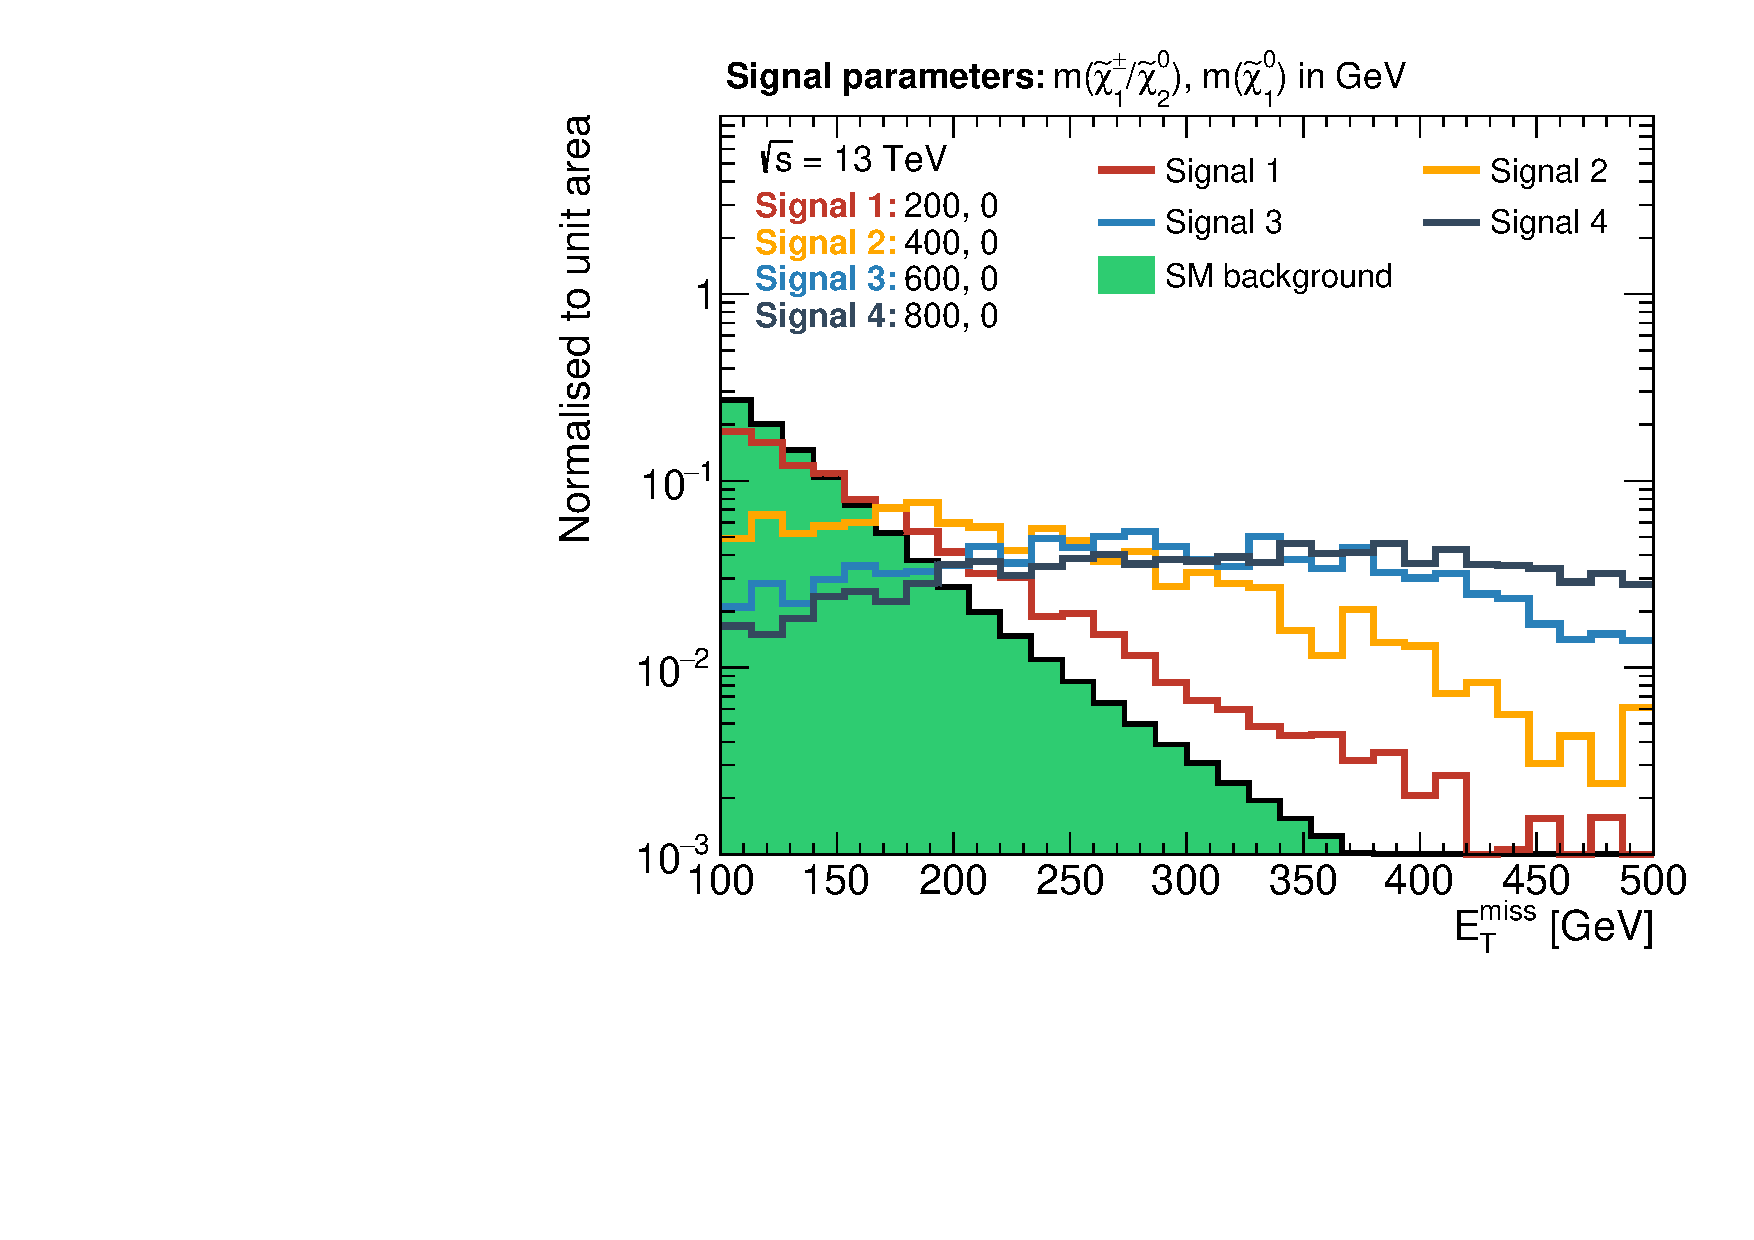
\includegraphics[width=0.8\textwidth]{high_mass/met}
	\end{subfigure}\hfill
	\begin{subfigure}[b]{0.5\linewidth}
		\centering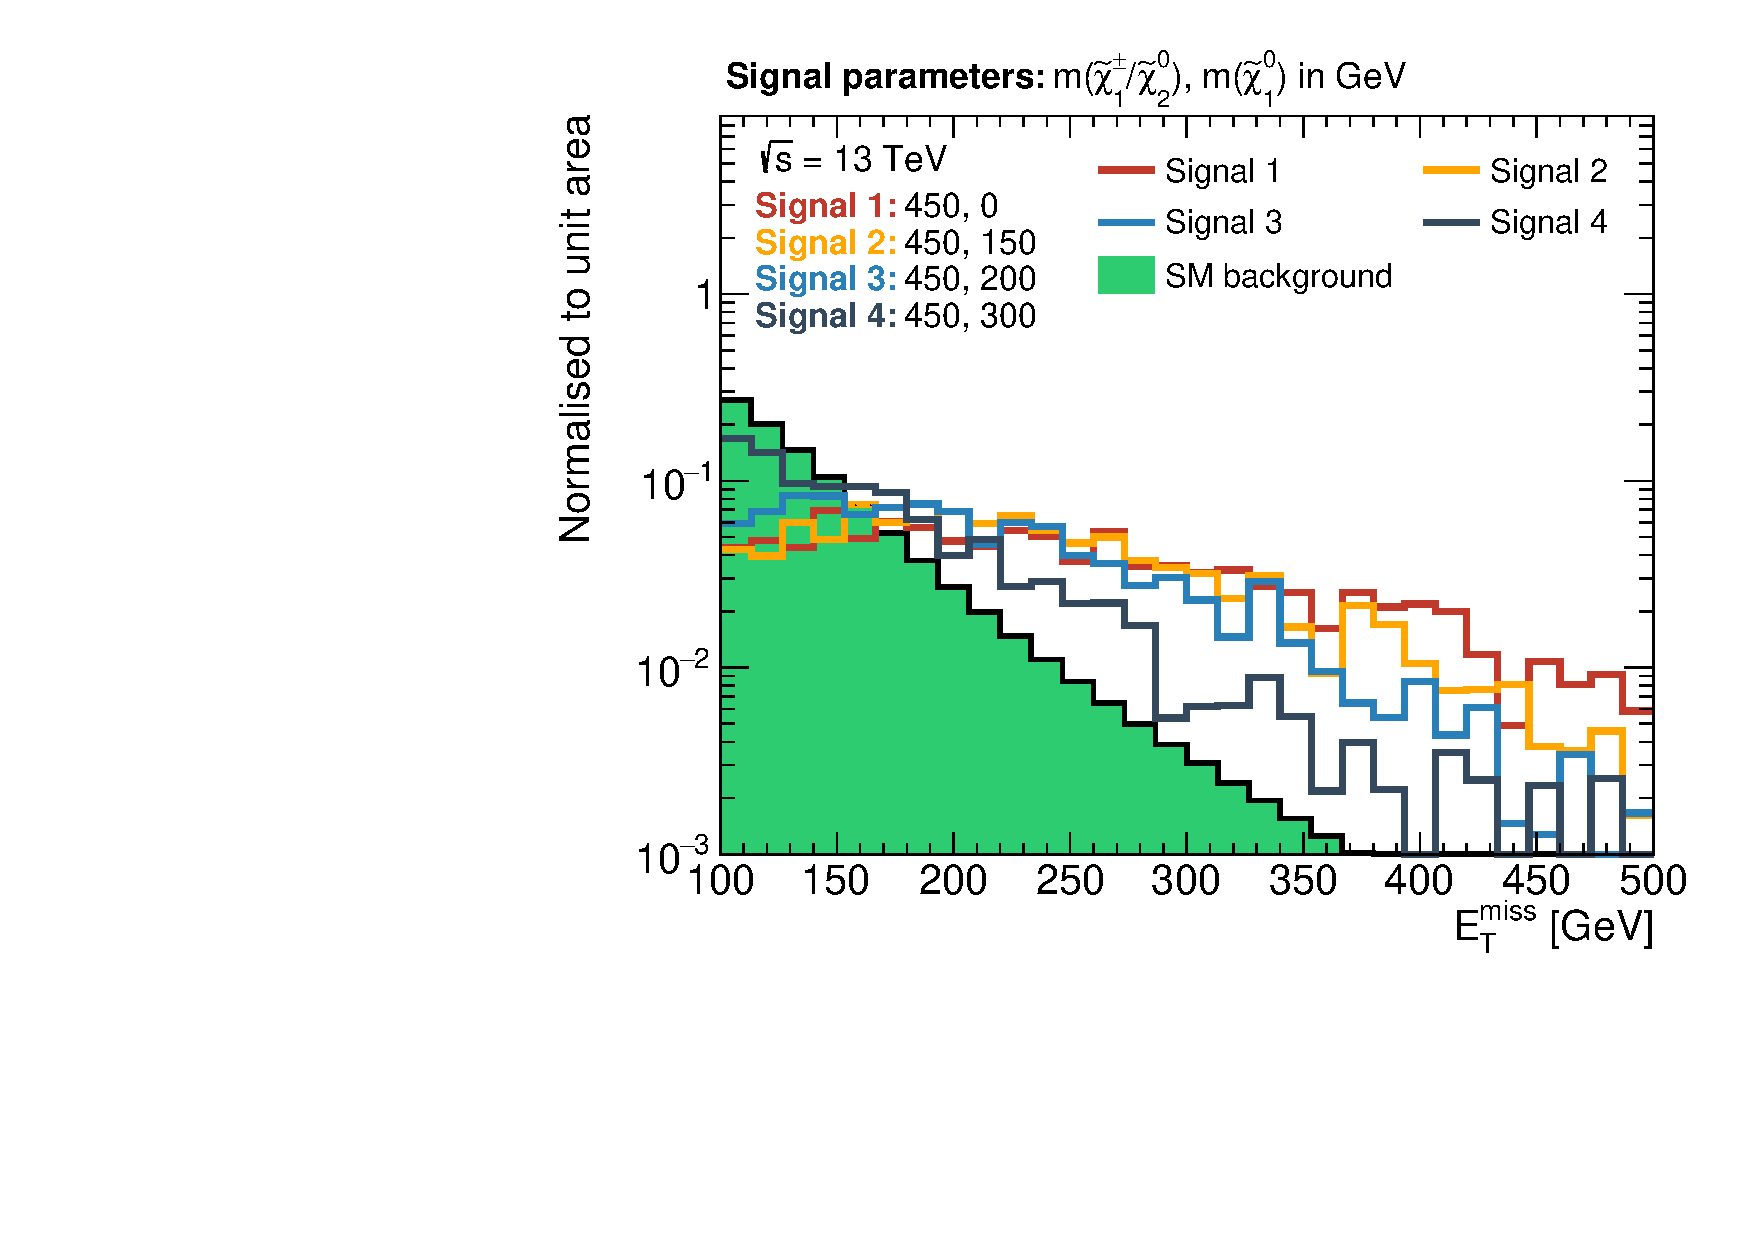
\includegraphics[width=0.8\textwidth]{mass_diff/met}
	\end{subfigure}\hfill
	\par\medskip
	\begin{subfigure}[b]{0.5\linewidth}
		\centering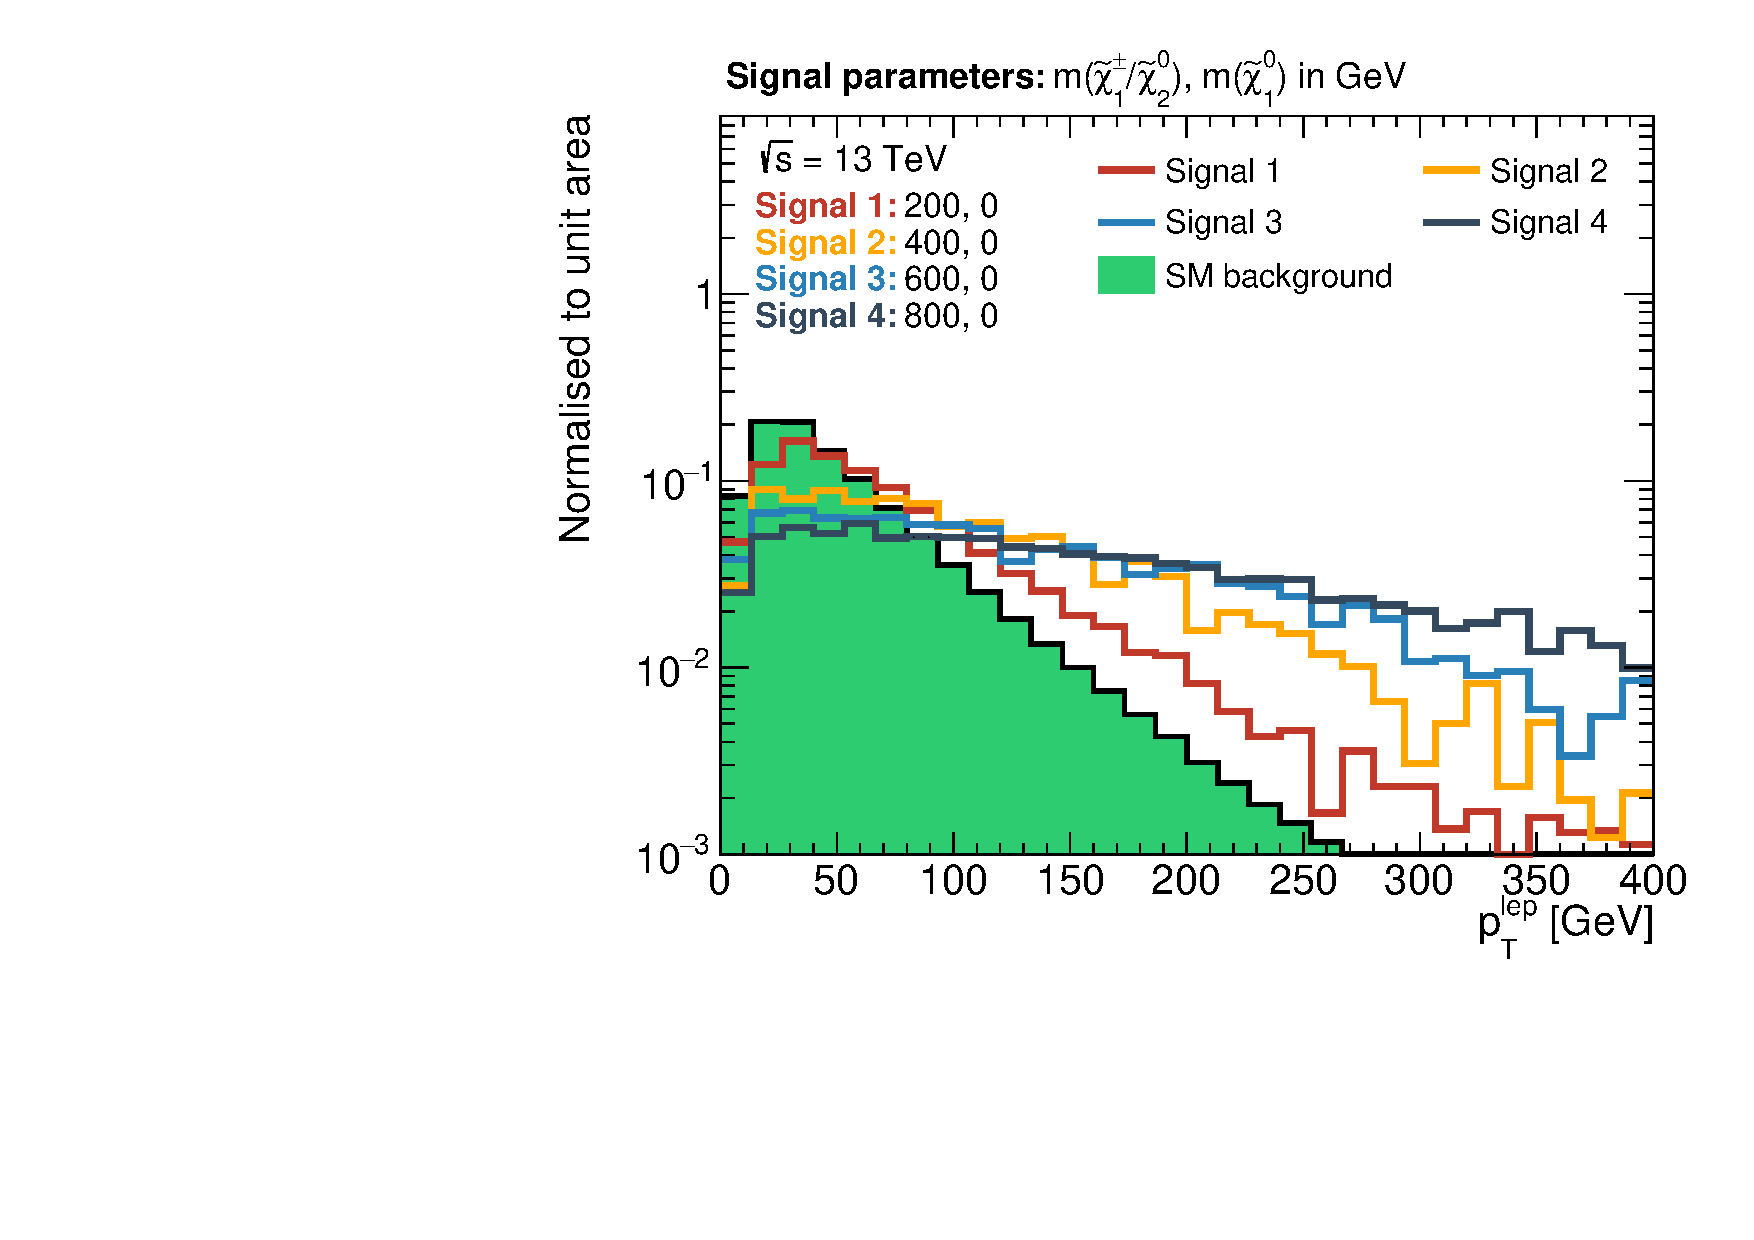
\includegraphics[width=0.8\textwidth]{high_mass/lep1Pt}
	\end{subfigure}\hfill
	\begin{subfigure}[b]{0.5\linewidth}
		\centering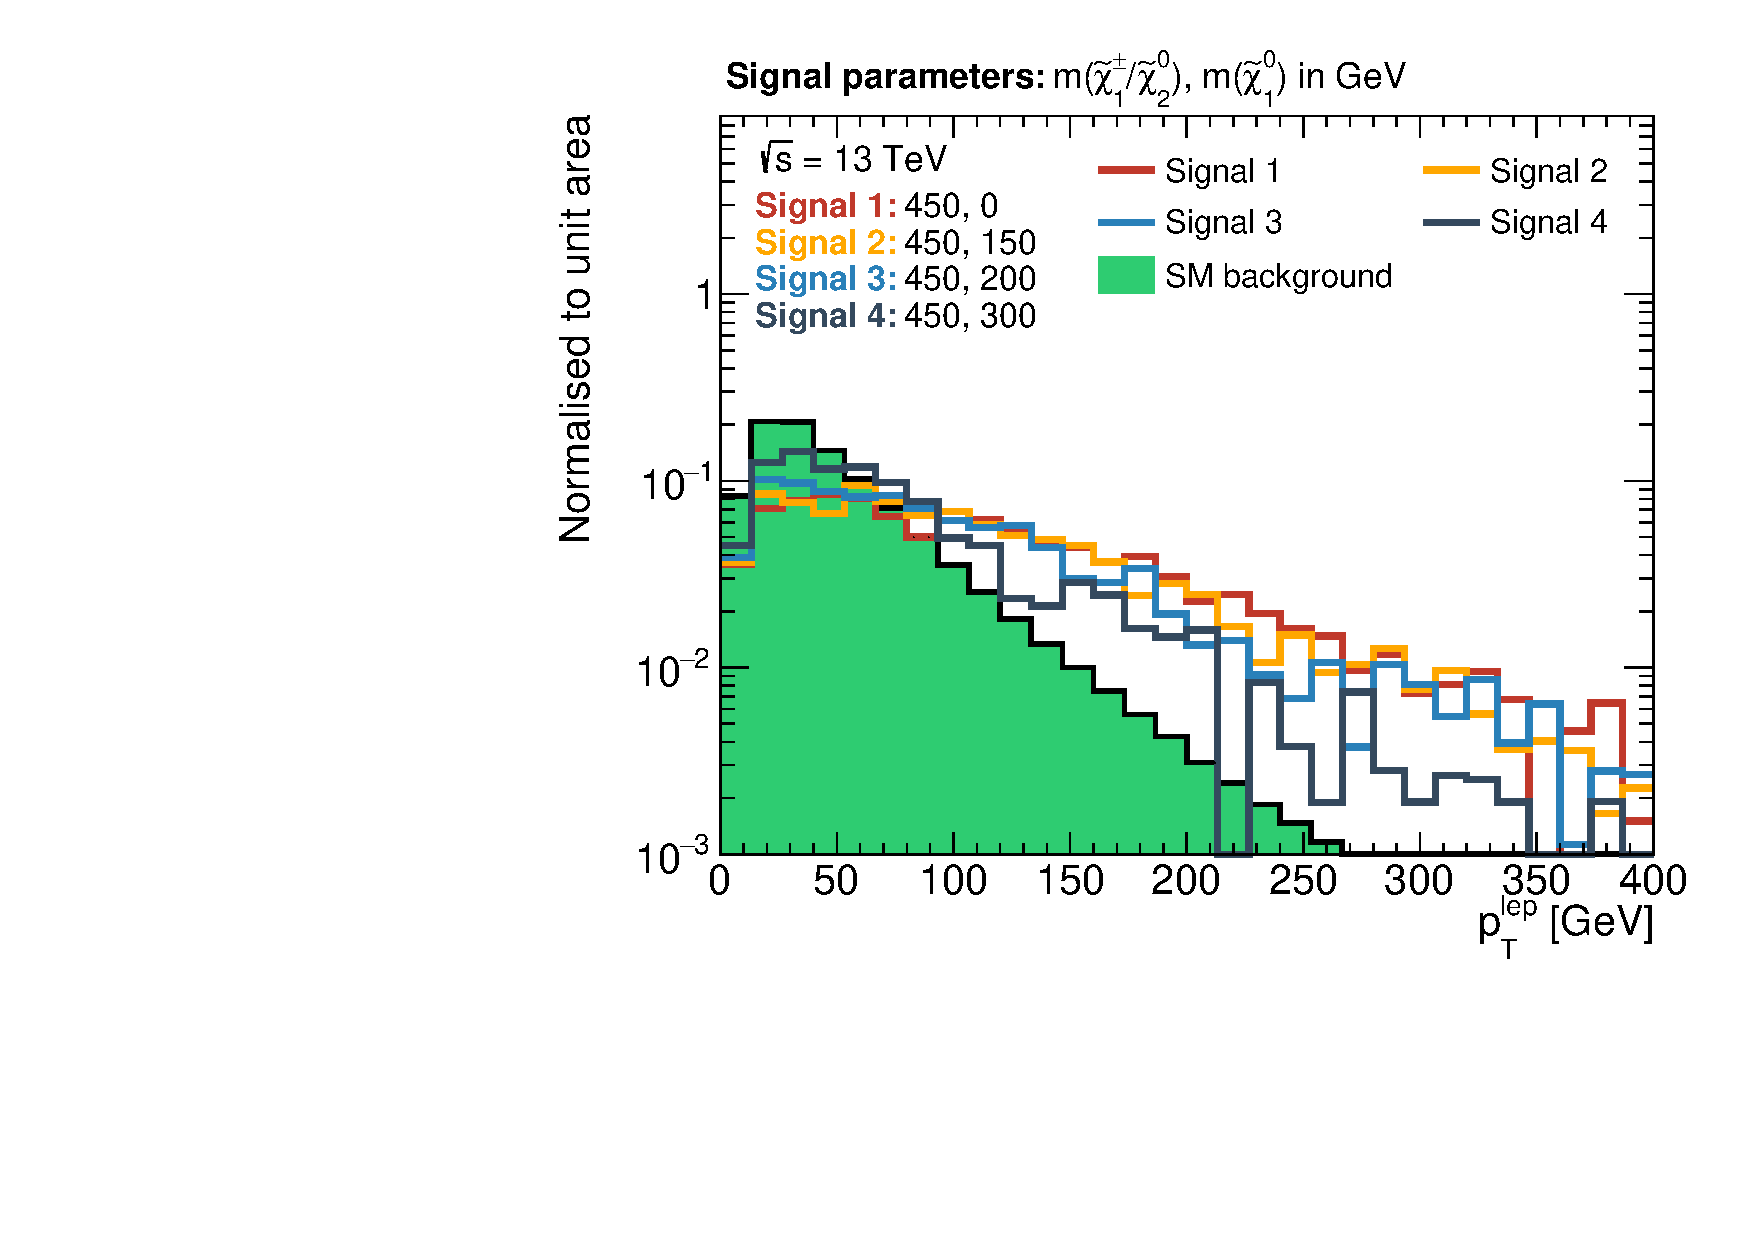
\includegraphics[width=0.8\textwidth]{mass_diff/lep1Pt}
	\end{subfigure}\hfill
	\par\medskip
	\begin{subfigure}[b]{0.5\linewidth}
		\centering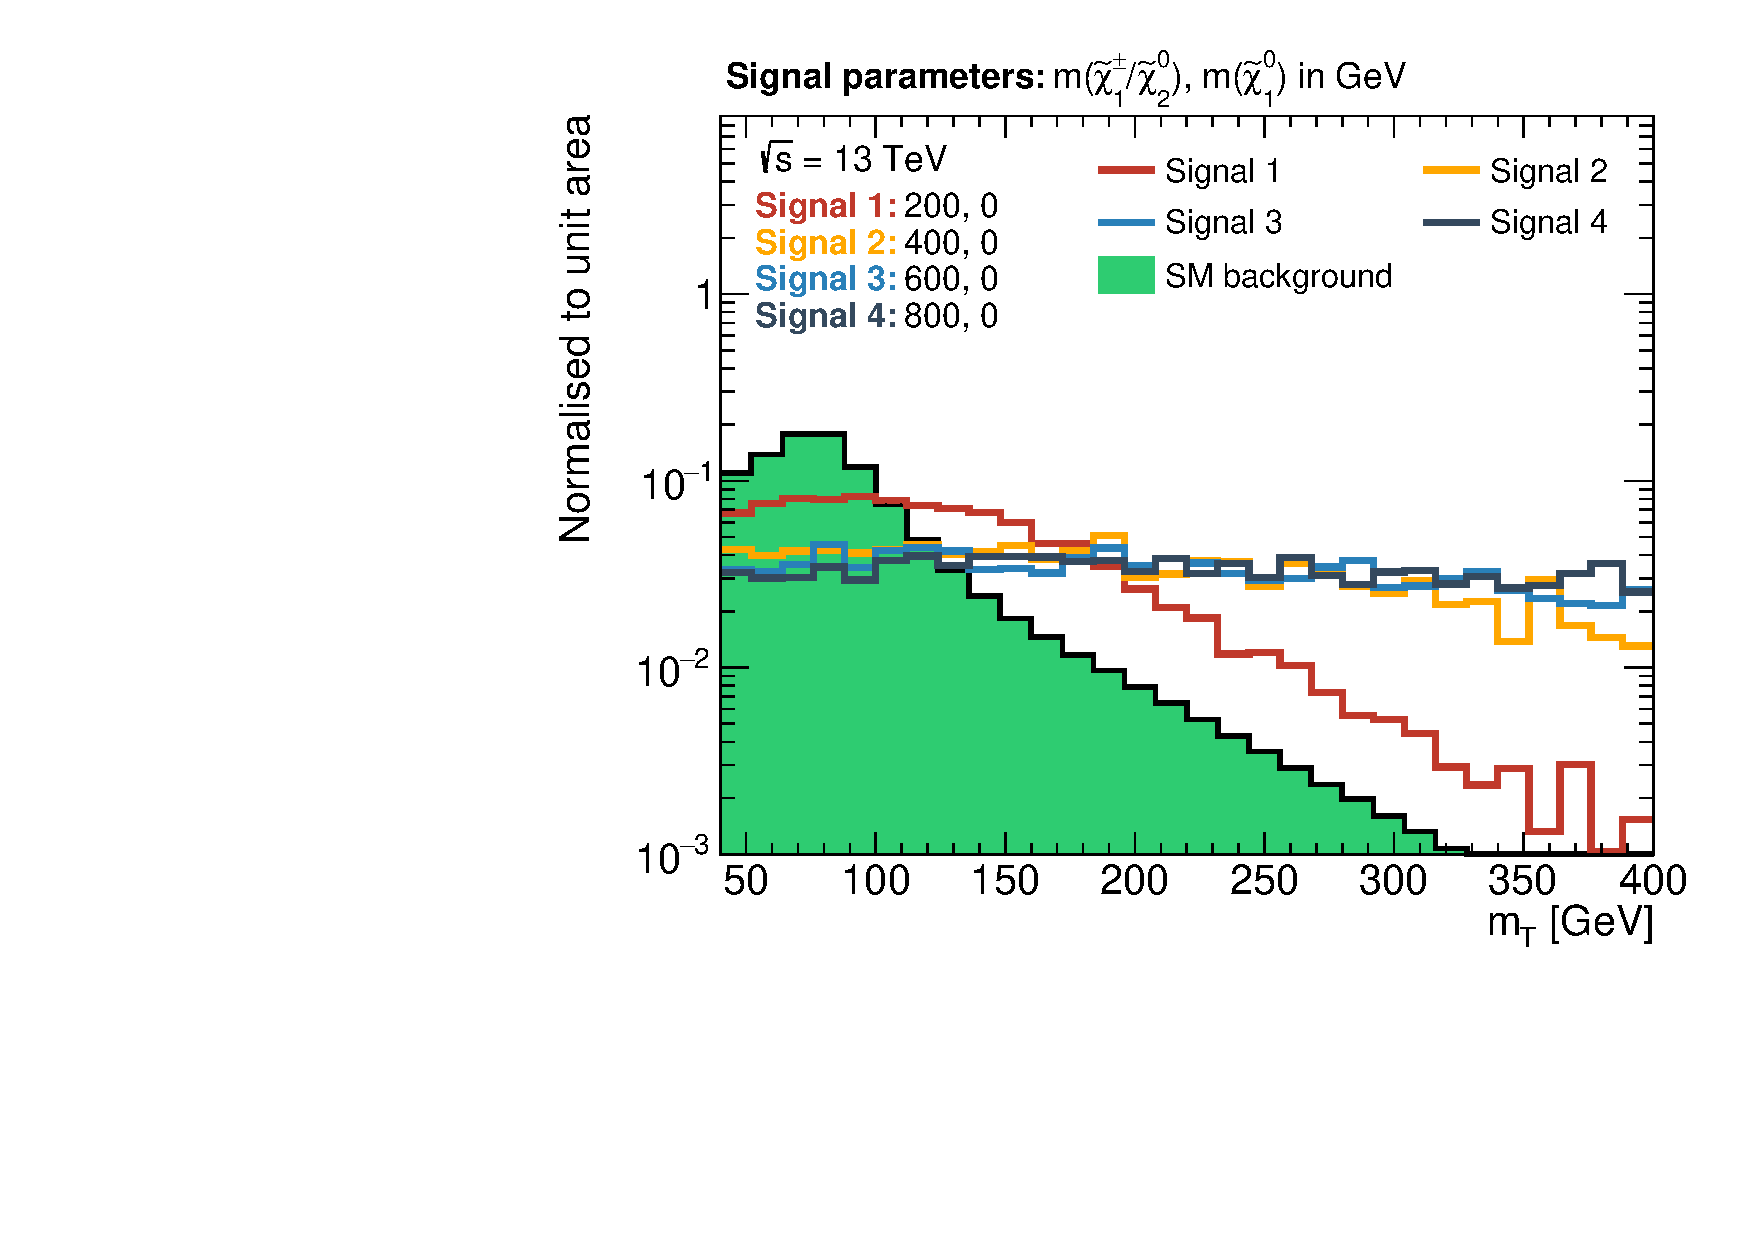
\includegraphics[width=0.8\textwidth]{high_mass/mt}
	\end{subfigure}\hfill
	\begin{subfigure}[b]{0.5\linewidth}
		\centering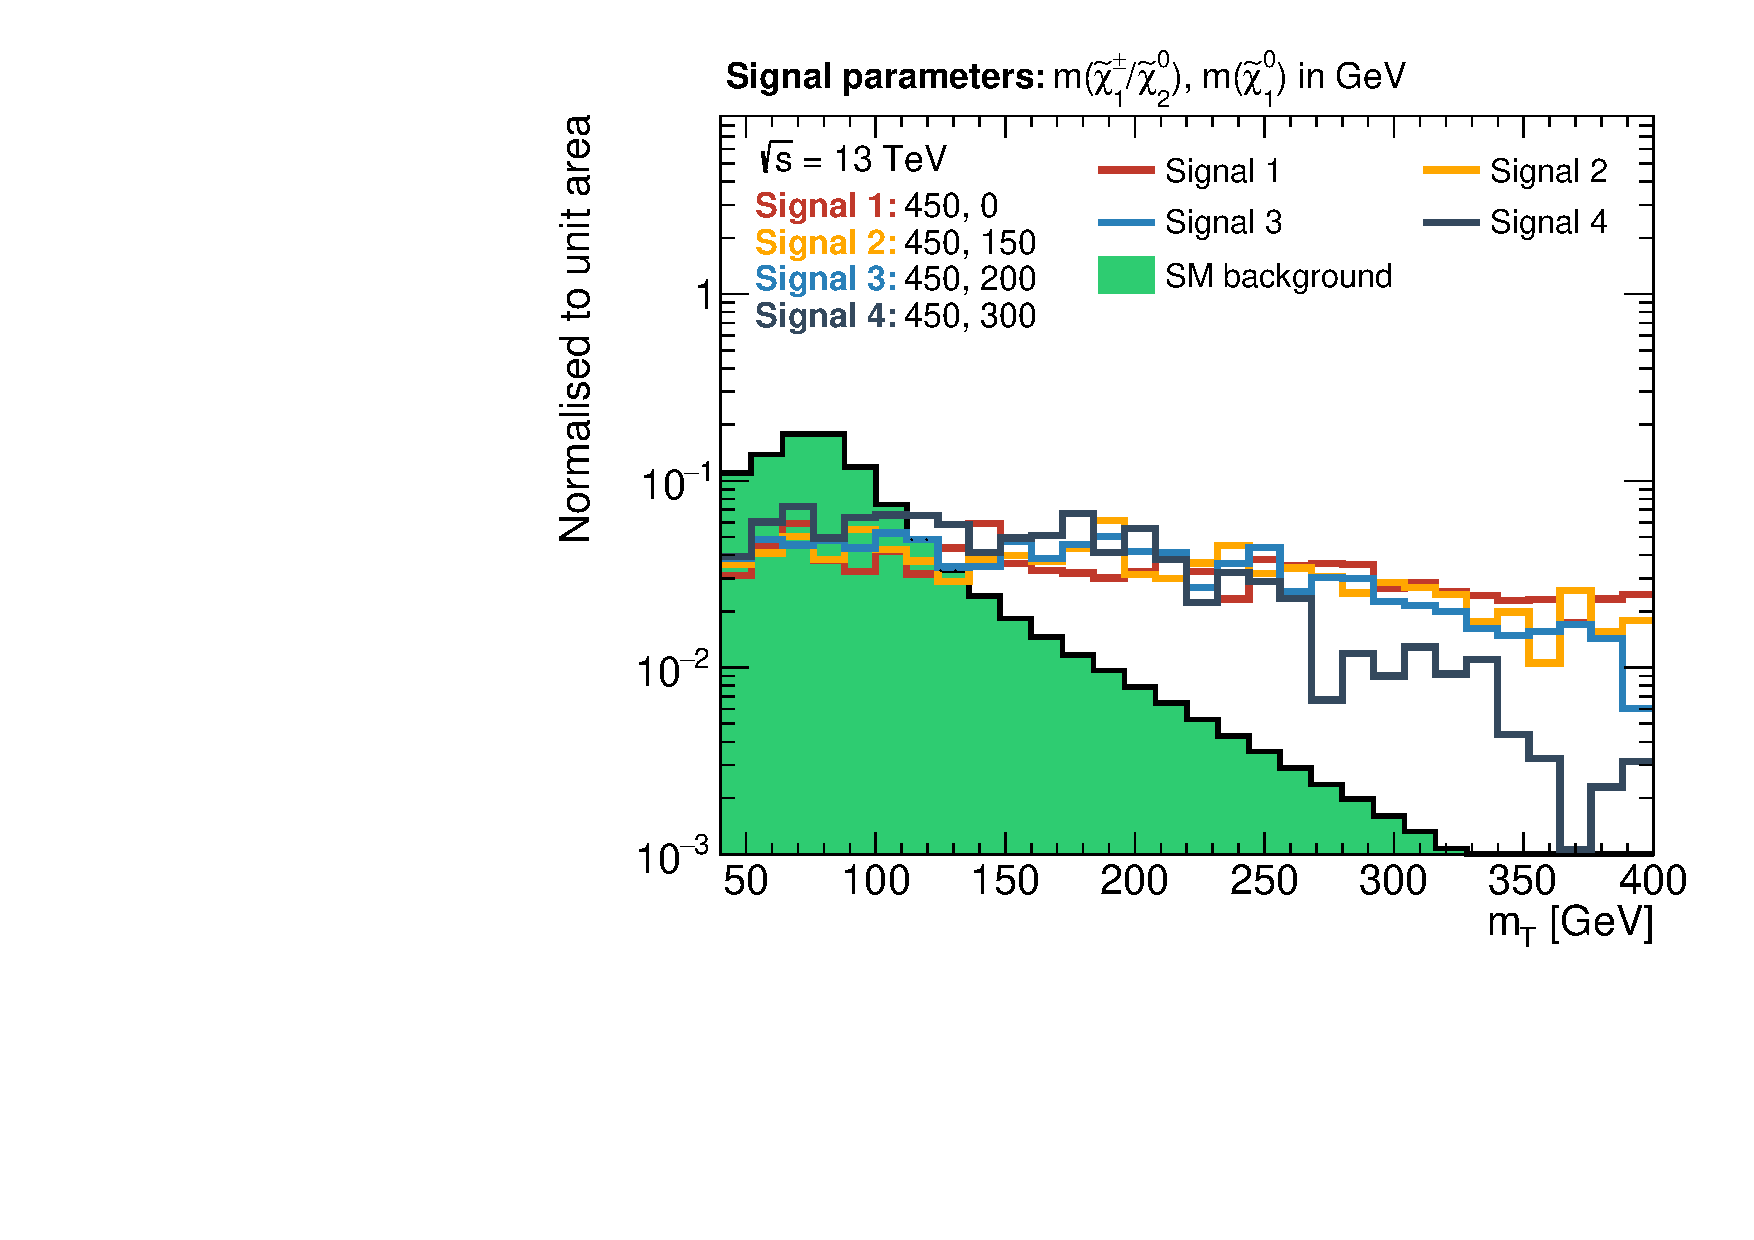
\includegraphics[width=0.8\textwidth]{mass_diff/mt}
	\end{subfigure}\hfill
	\par\medskip
	\begin{subfigure}[b]{0.5\linewidth}
		\centering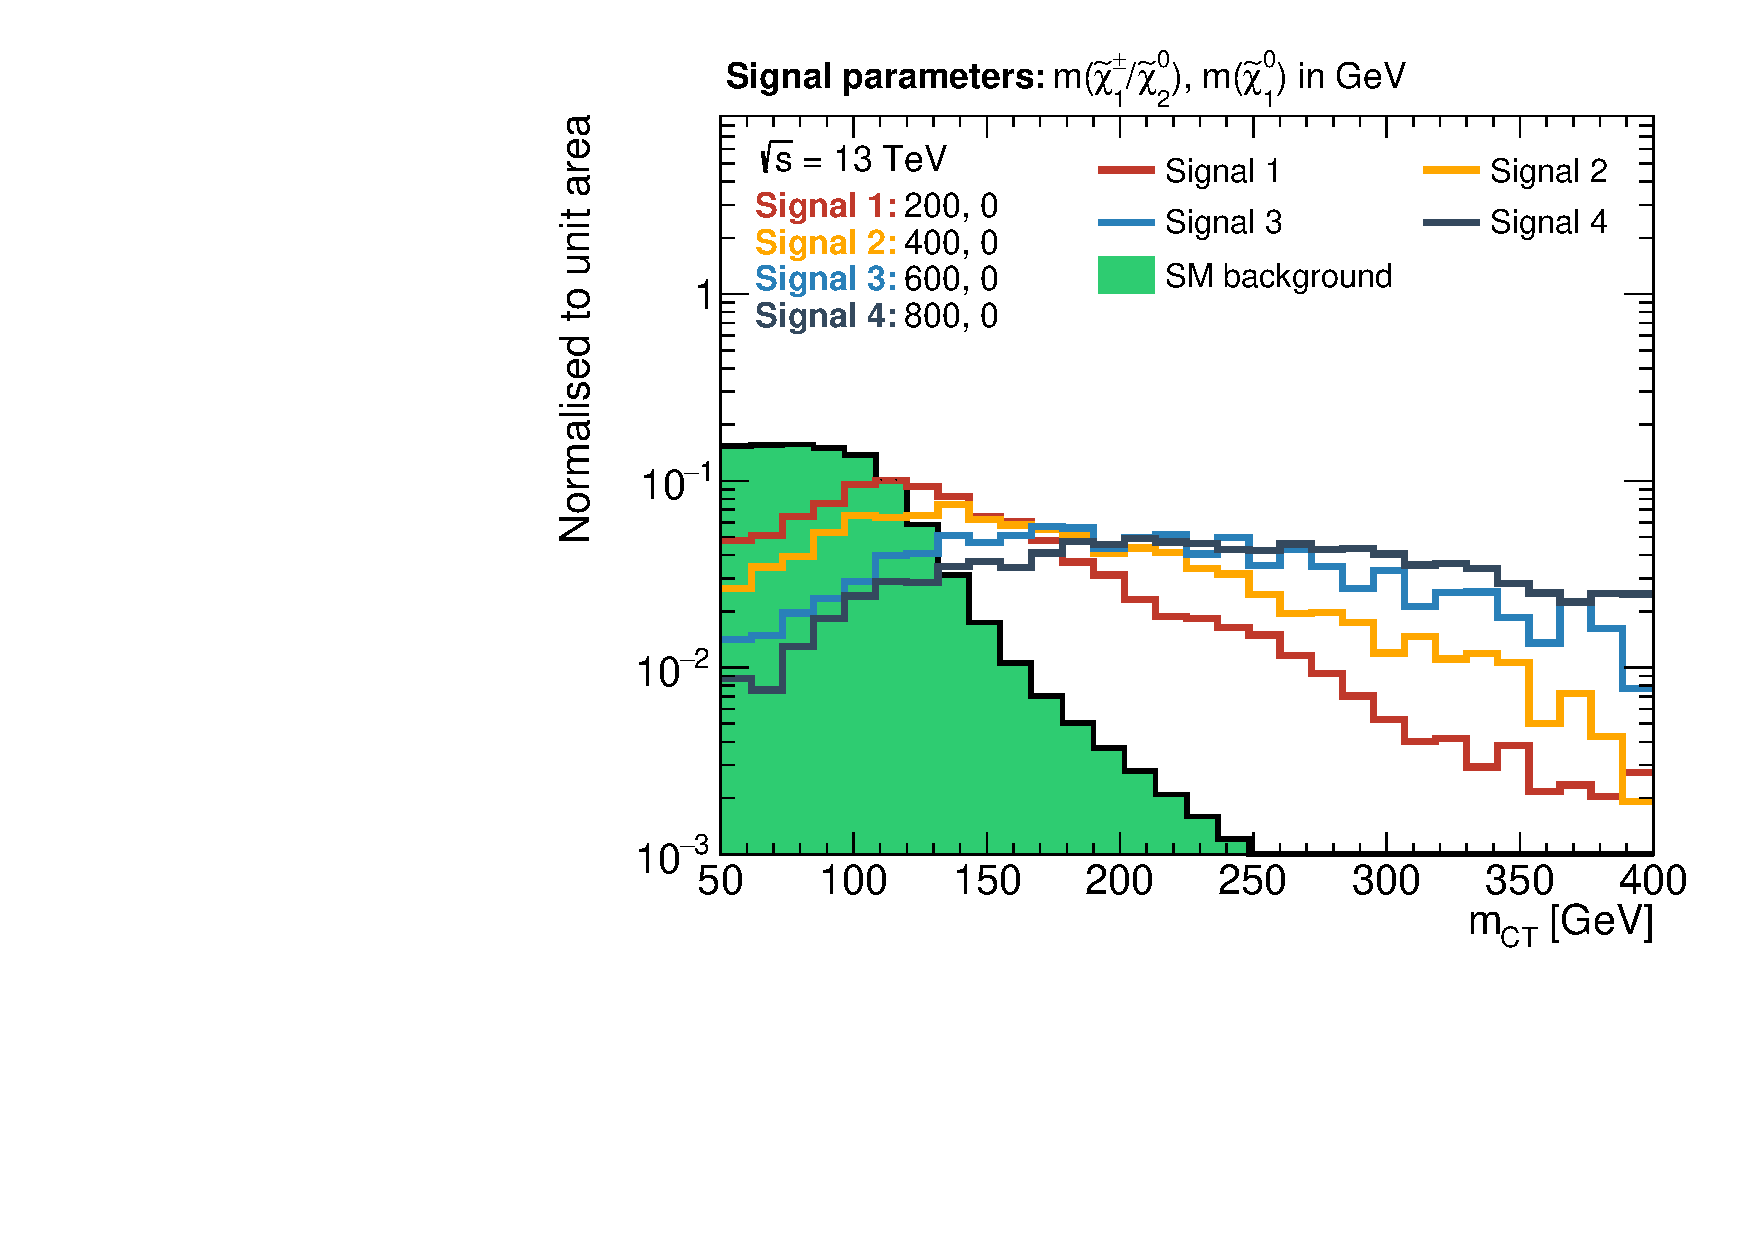
\includegraphics[width=0.8\textwidth]{high_mass/mct}
	\end{subfigure}\hfill
	\begin{subfigure}[b]{0.5\linewidth}
		\centering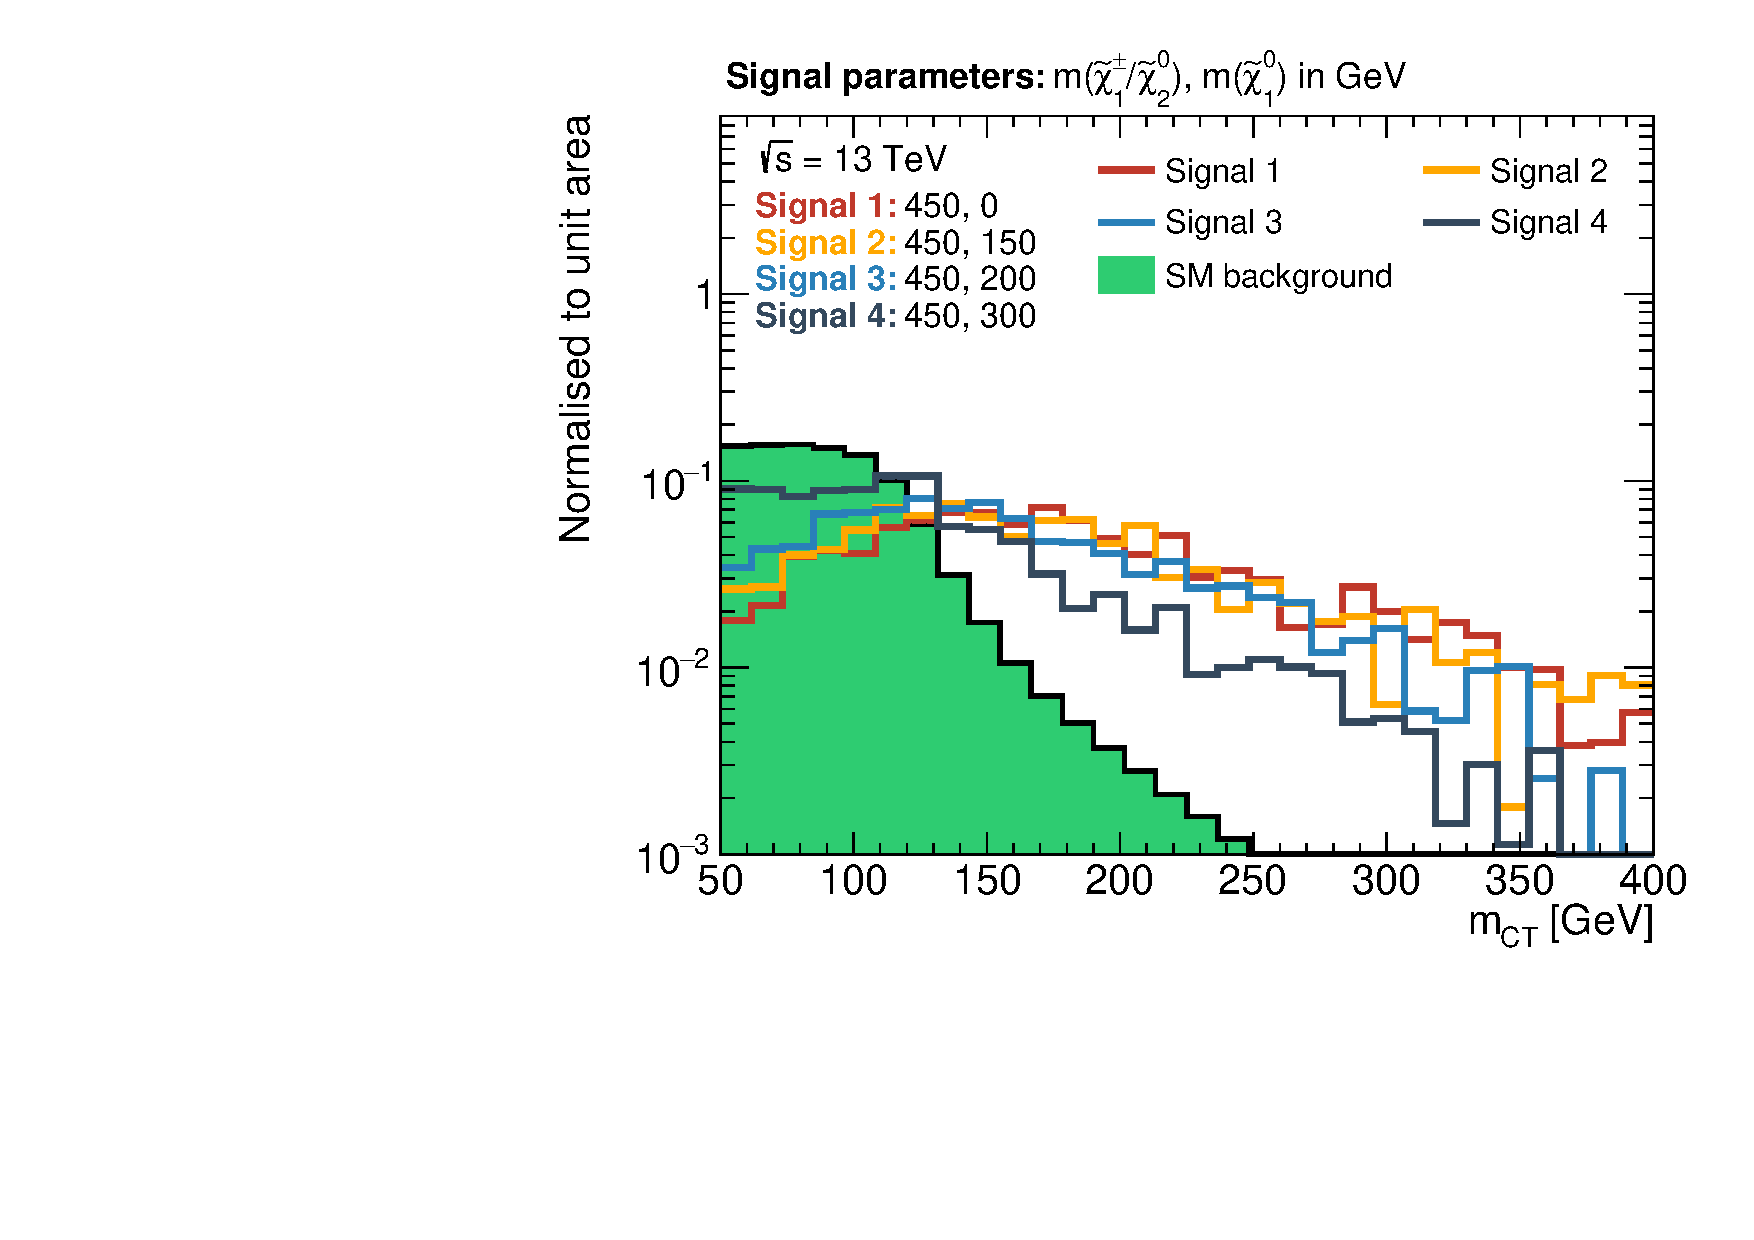
\includegraphics[width=0.8\textwidth]{mass_diff/mct}
	\end{subfigure}

	\caption{Dependence of some of the kinematic observables on the \mbox{$\charg$/$\neutr$} mass scale (left) and \mbox{$\charg$/$\neutr$}--$\lsp$ mass differences (right). The simulated \gls{sm} backgrounds are stacked on top of each other and summarised in a single `SM' histogram. Distributions from representative signal models with the quoted mass parameters are overlaid. In order to emphasise the shape differences, both total background and signal distributions are normalised to unity. A preselection requiring a lepton, at least two jets and $\etmiss > \SI{100}{\GeV}$ is applied.}\label{fig:norm_obs_app}
\end{figure}

\begin{figure}
	\centering
	\begin{subfigure}[b]{0.5\linewidth}
		\centering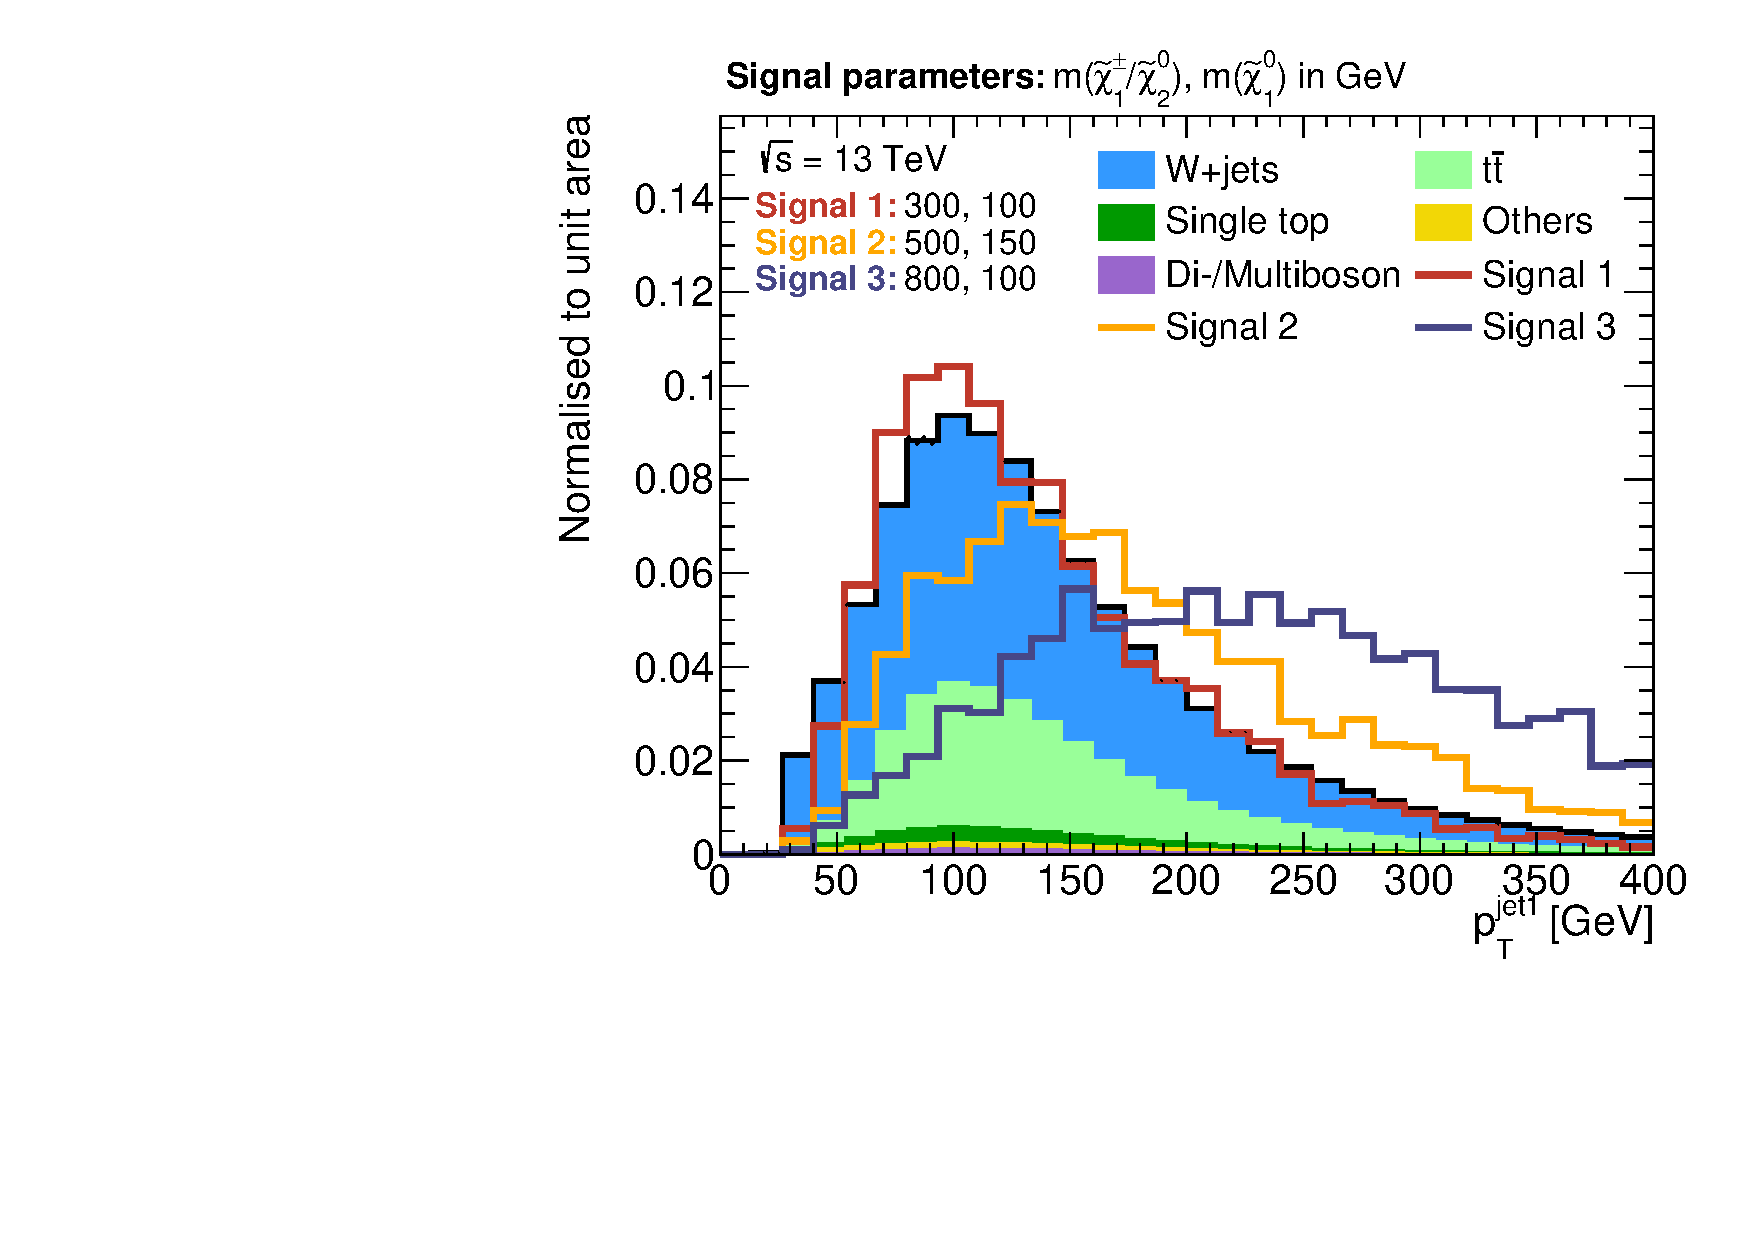
\includegraphics[width=0.8\textwidth]{presel/jet1Pt}
	\end{subfigure}\hfill
	\begin{subfigure}[b]{0.5\linewidth}
		\centering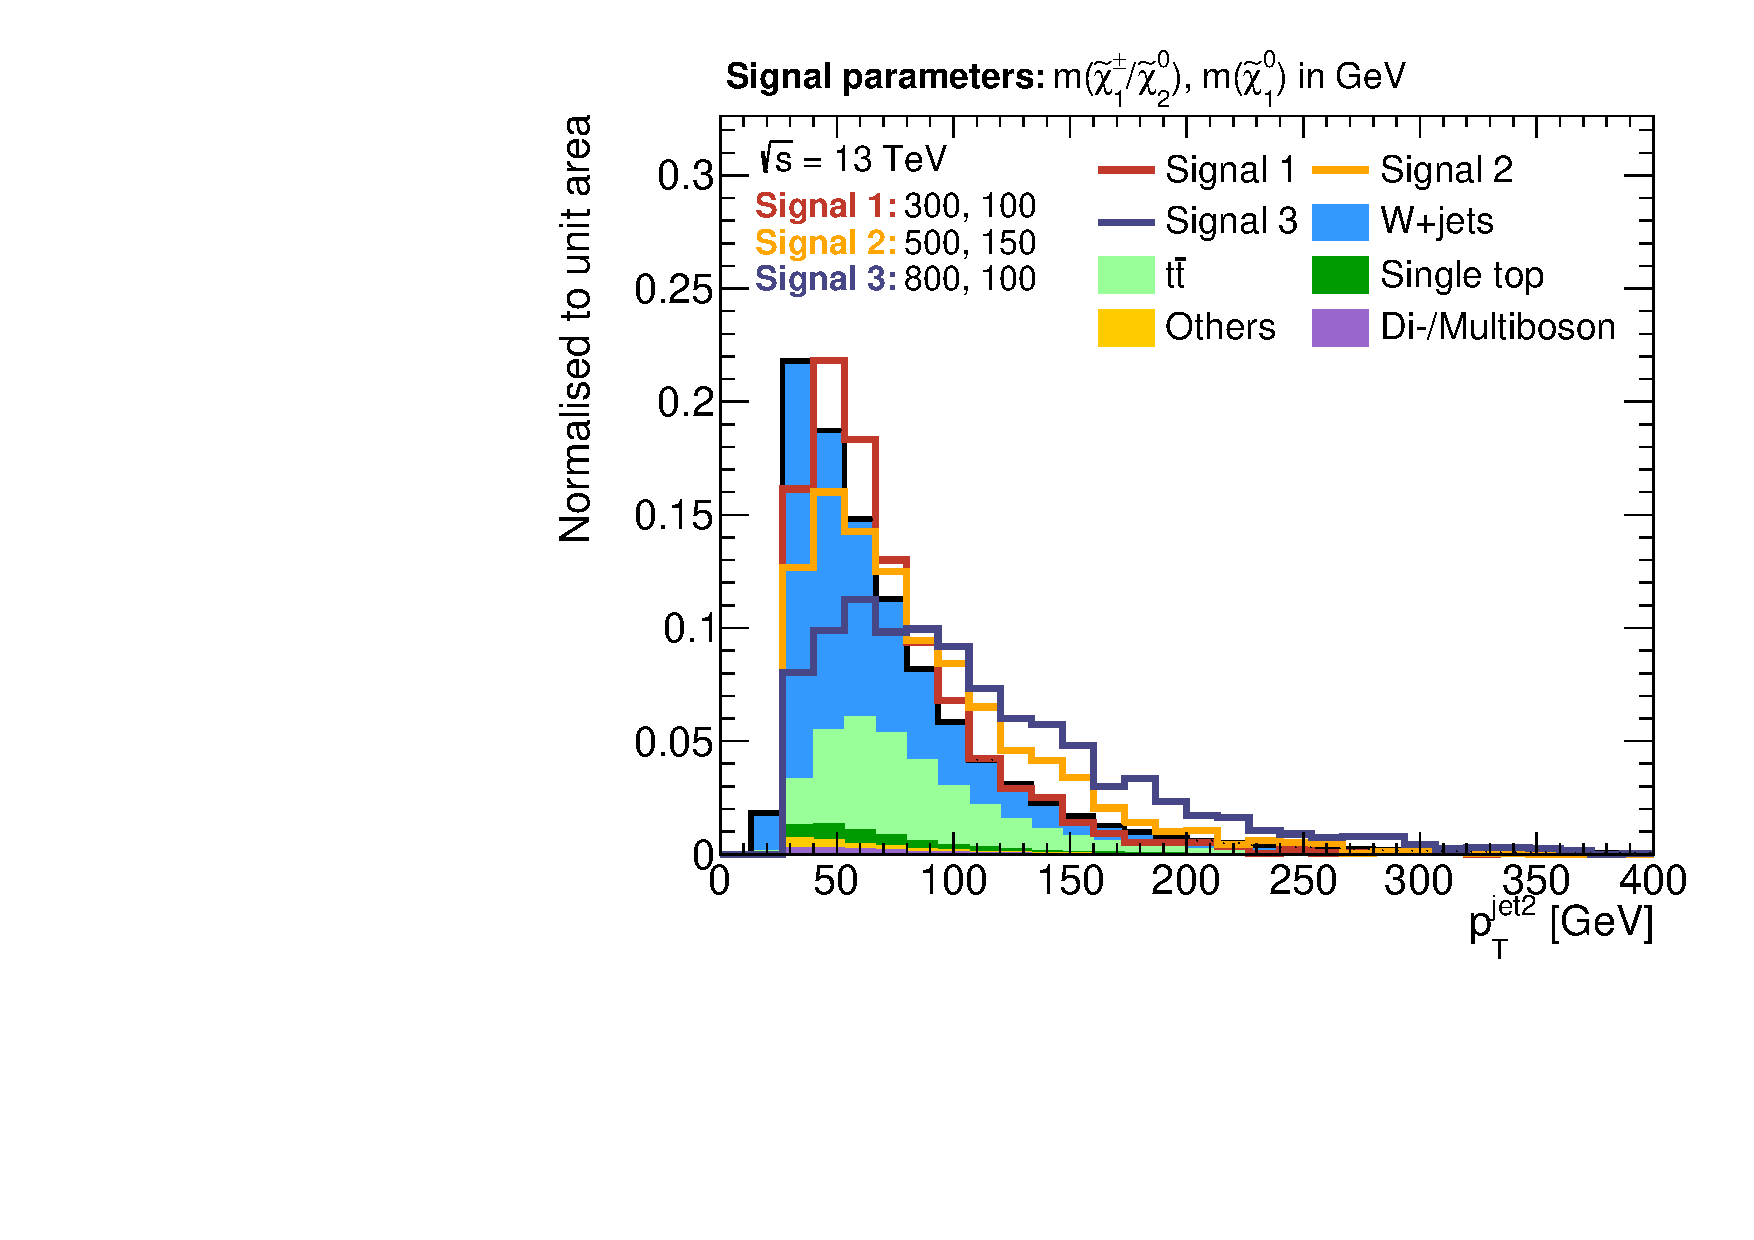
\includegraphics[width=0.8\textwidth]{presel/jet2Pt}
	\end{subfigure}\hfill
	\par\medskip
	\begin{subfigure}[b]{0.5\linewidth}
		\centering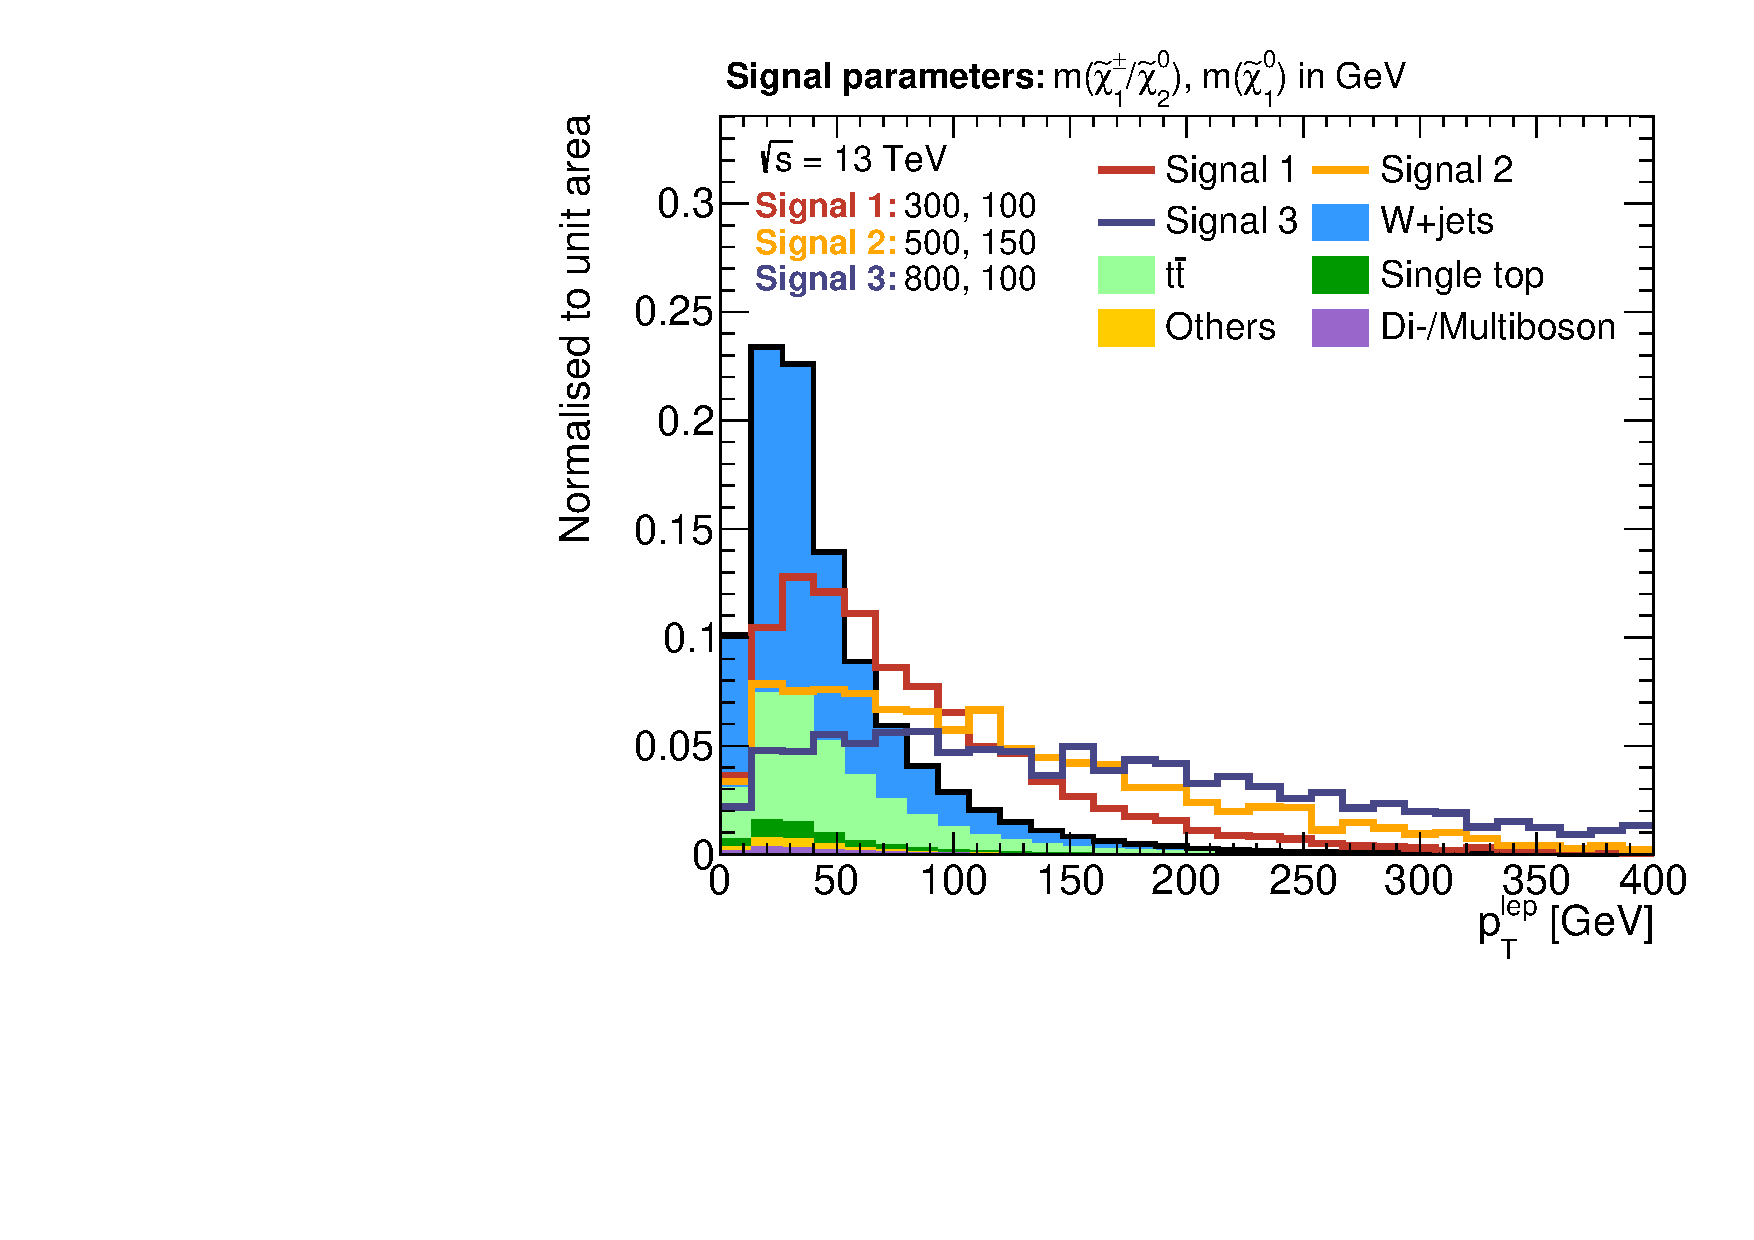
\includegraphics[width=0.8\textwidth]{presel/lep1Pt}
	\end{subfigure}\hfill
	\begin{subfigure}[b]{0.5\linewidth}
		\centering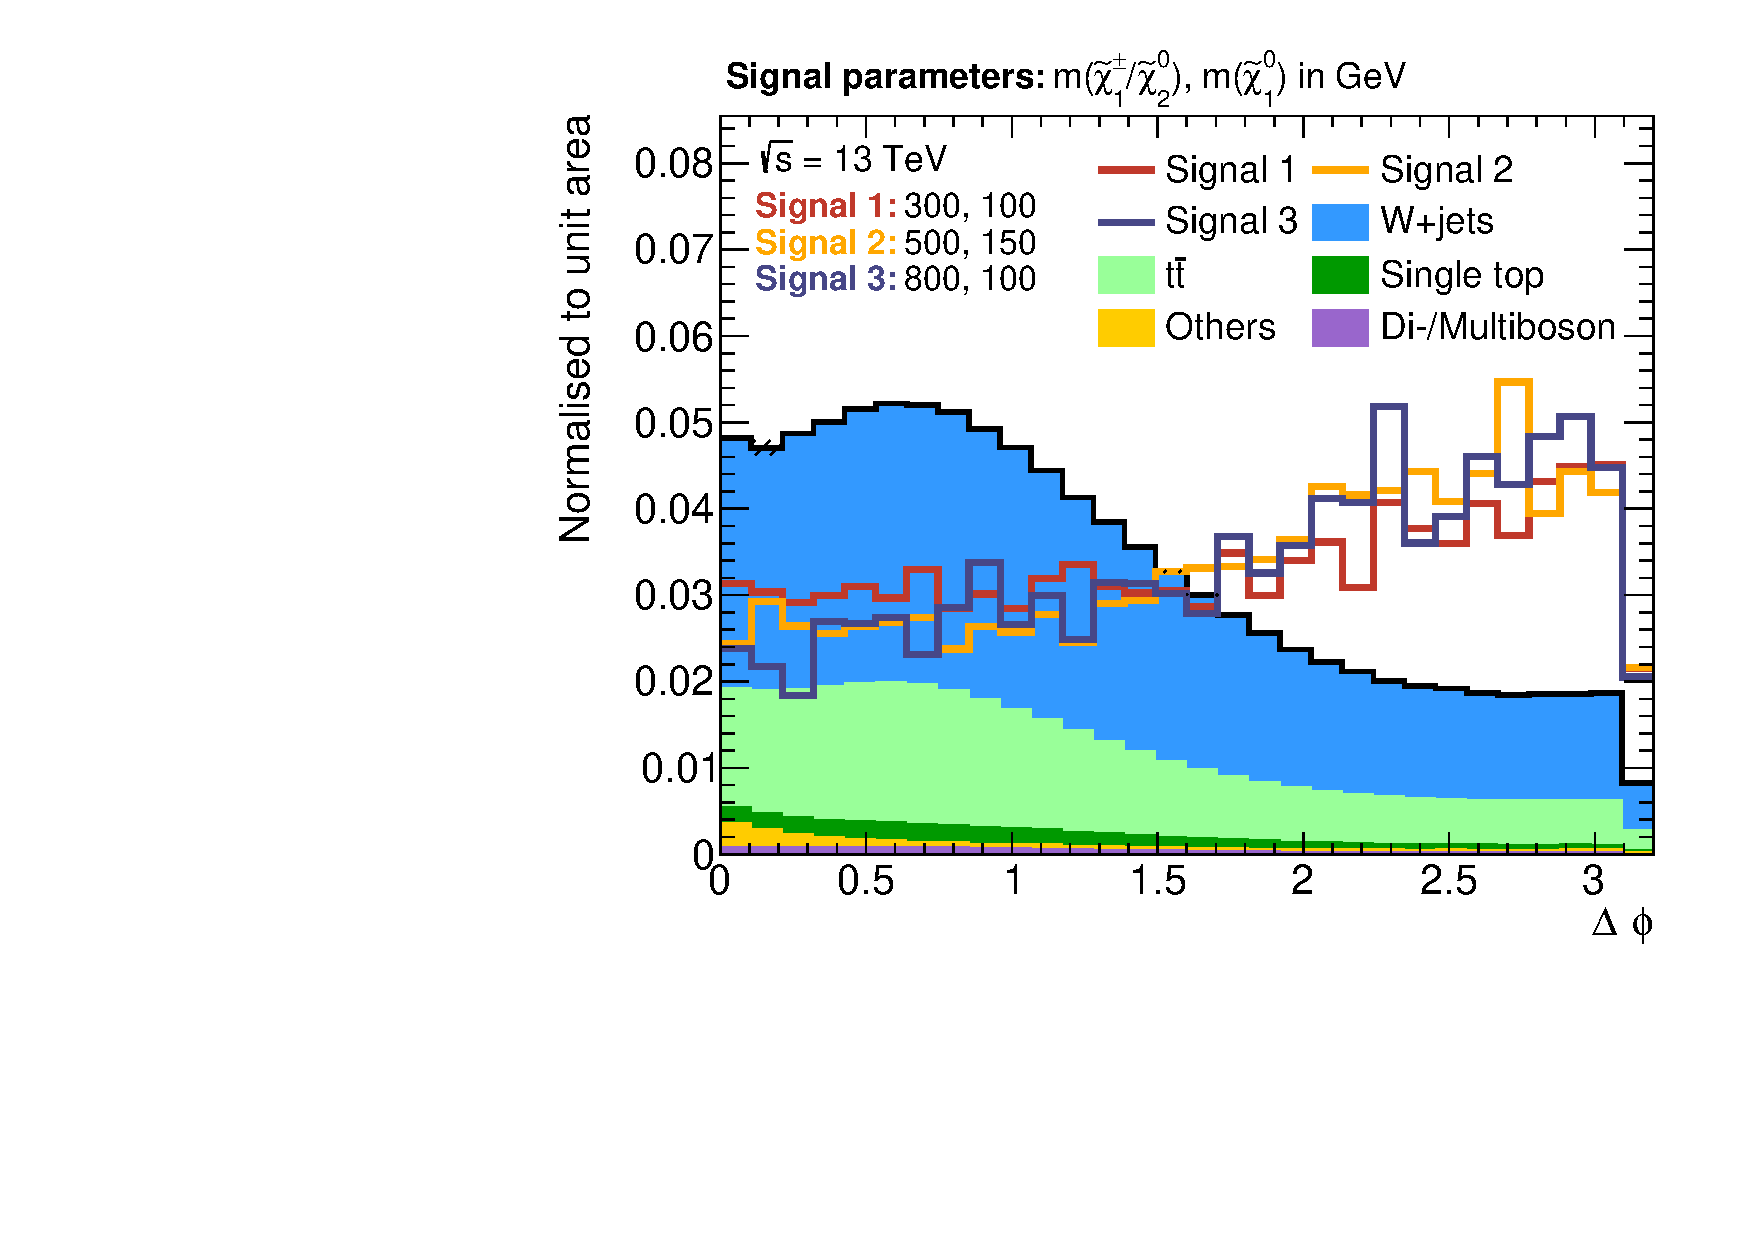
\includegraphics[width=0.8\textwidth]{presel/dphimetlep}
	\end{subfigure}\hfill
	\par\medskip
	\begin{subfigure}[b]{0.5\linewidth}
		\centering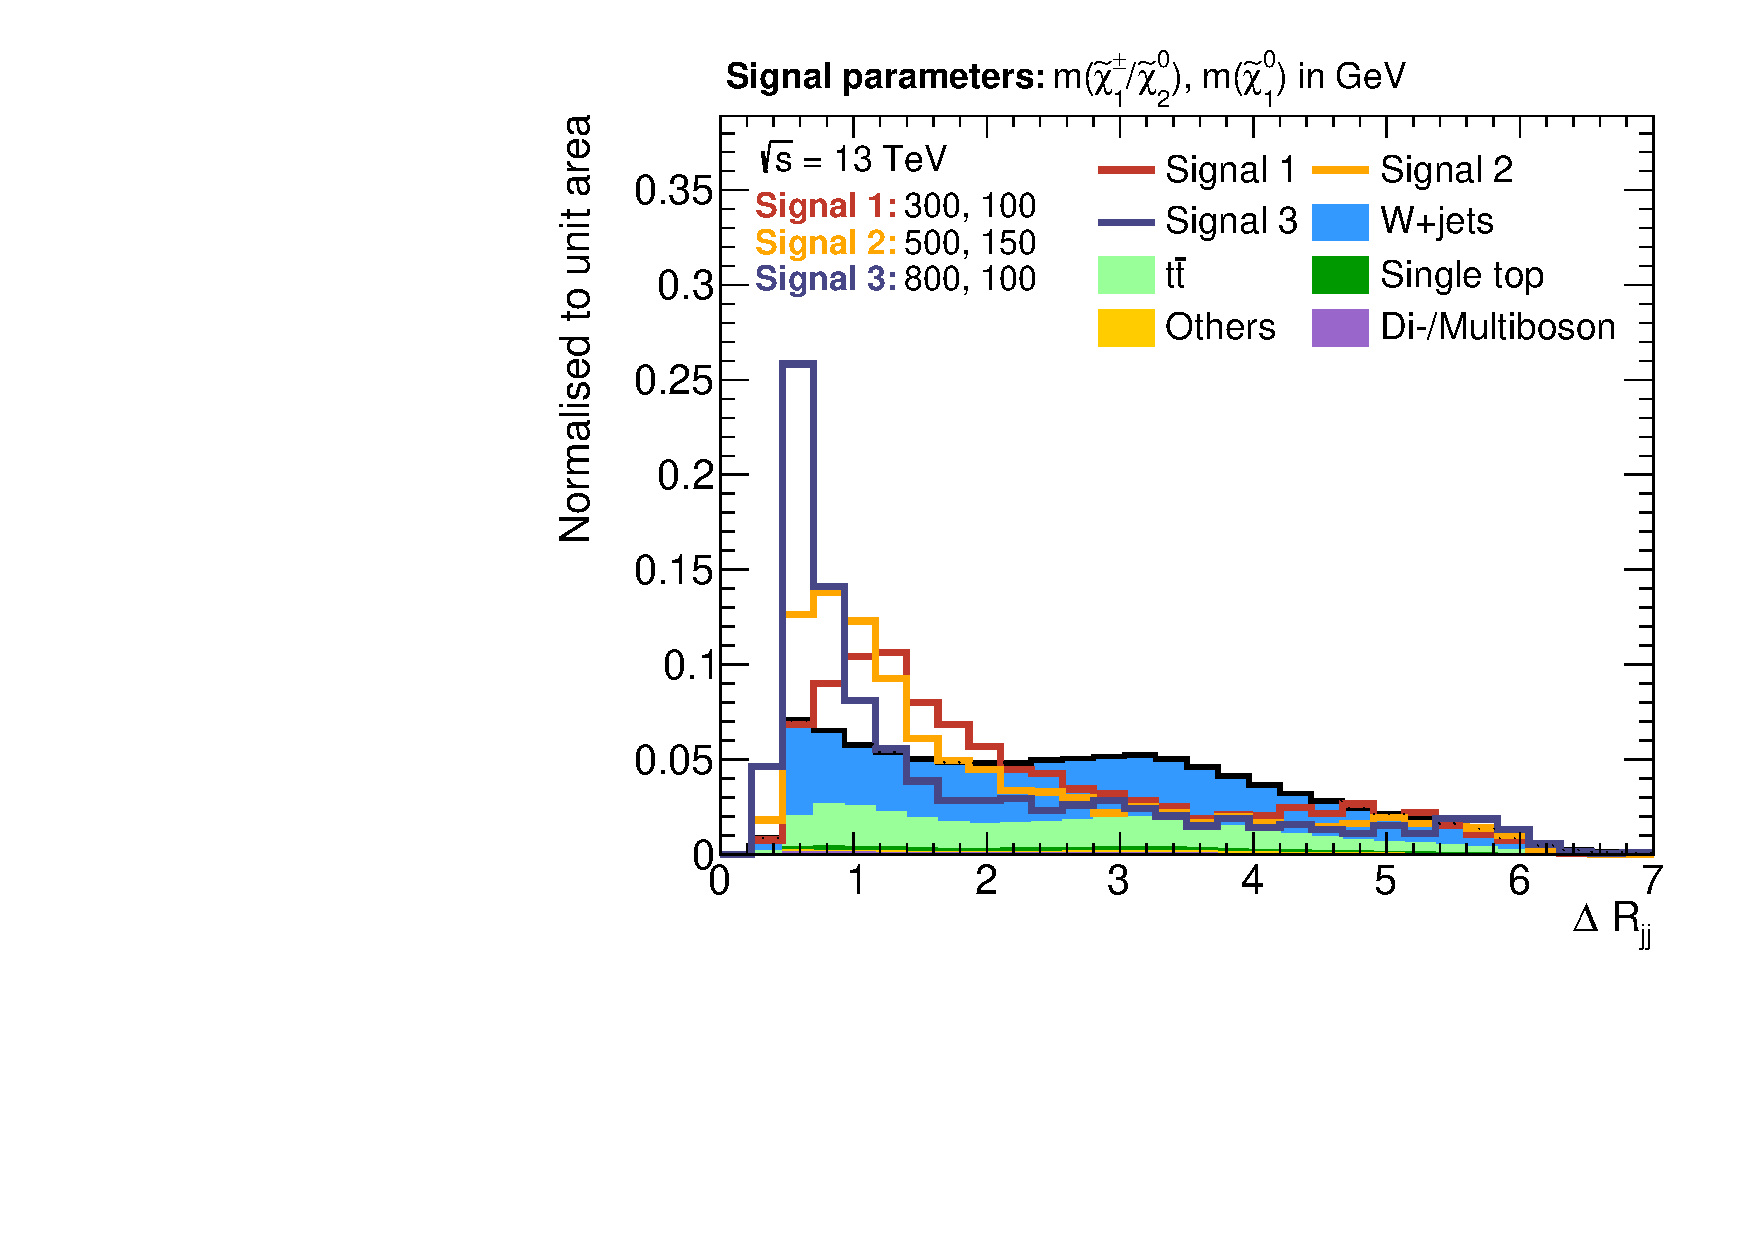
\includegraphics[width=0.8\textwidth]{presel/dRJet}
	\end{subfigure}\hfill
	\begin{subfigure}[b]{0.5\linewidth}
		\centering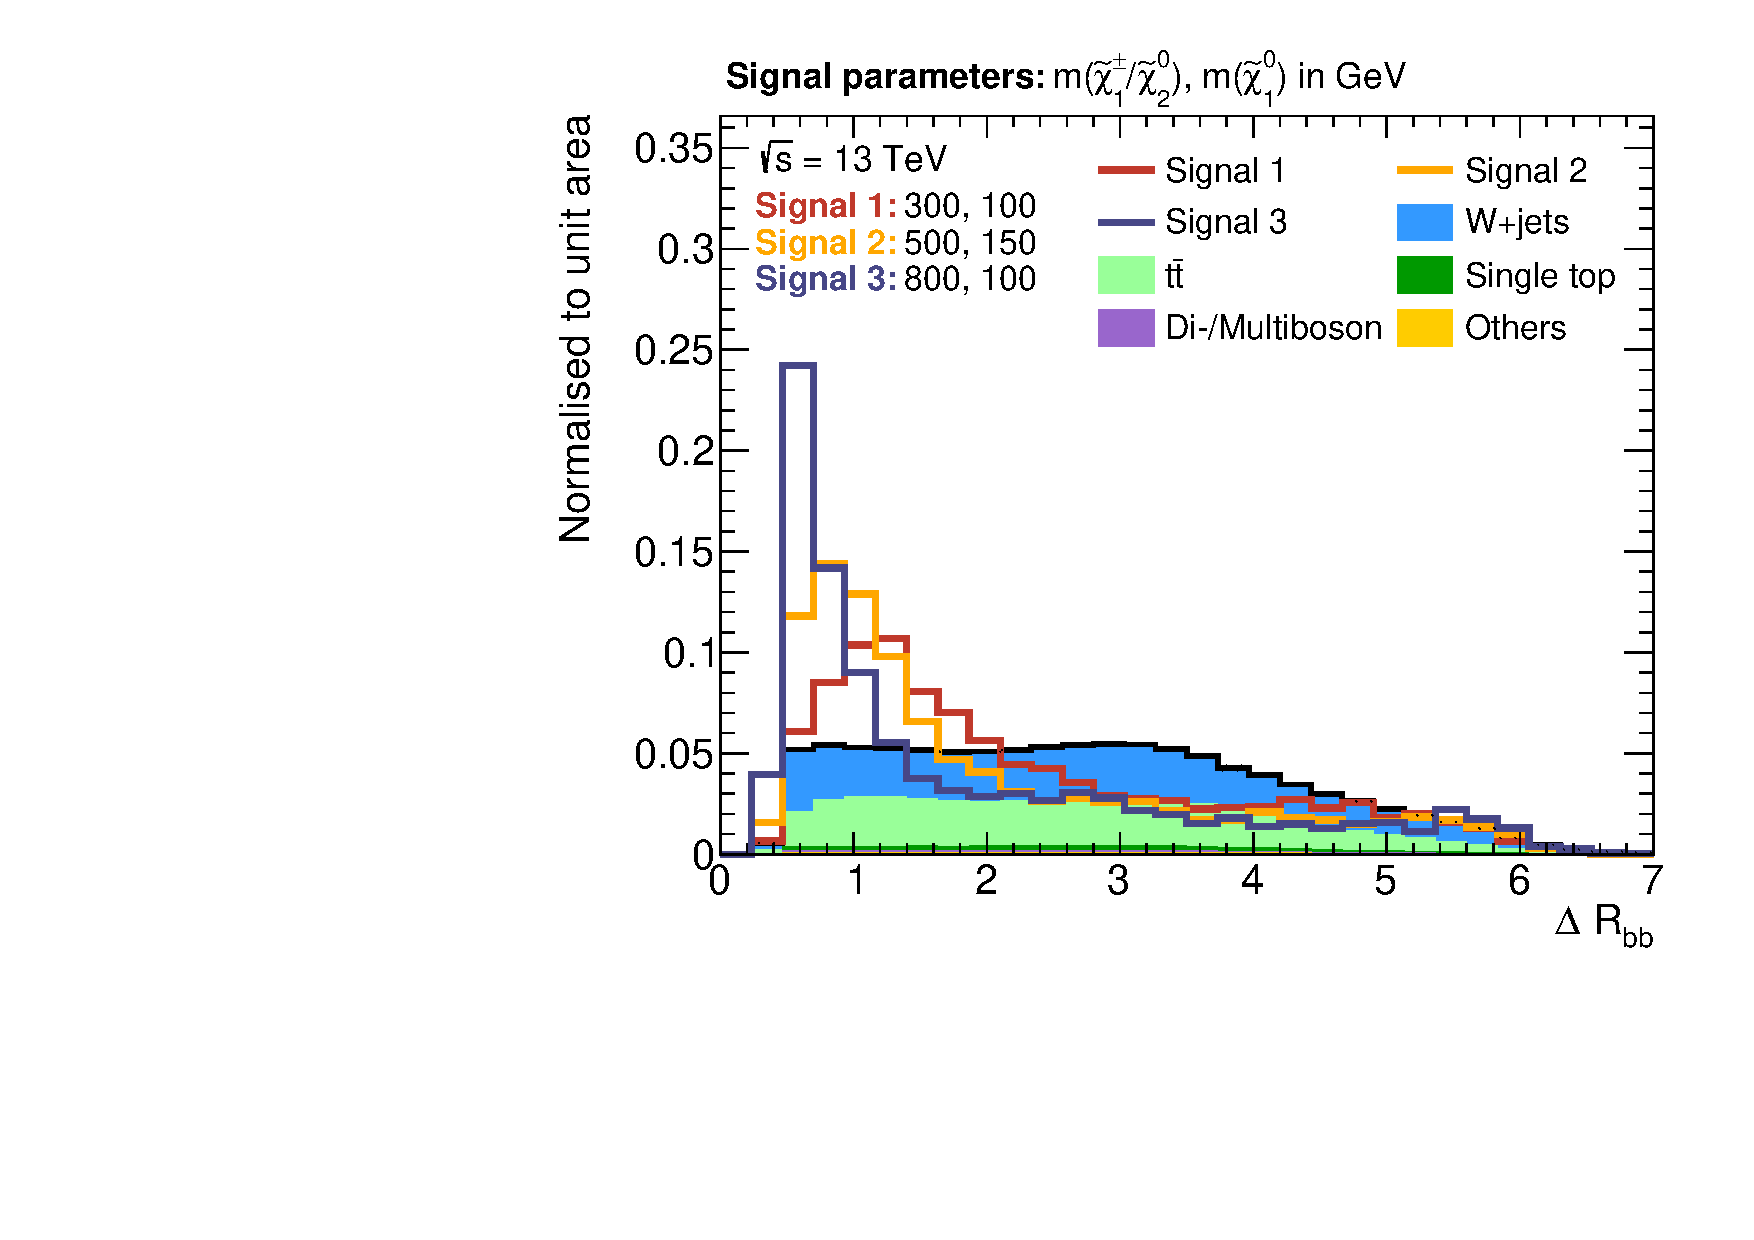
\includegraphics[width=0.8\textwidth]{presel/dRJBet}
	\end{subfigure}\hfill
	\par\medskip
	\begin{subfigure}[b]{0.5\linewidth}
		\centering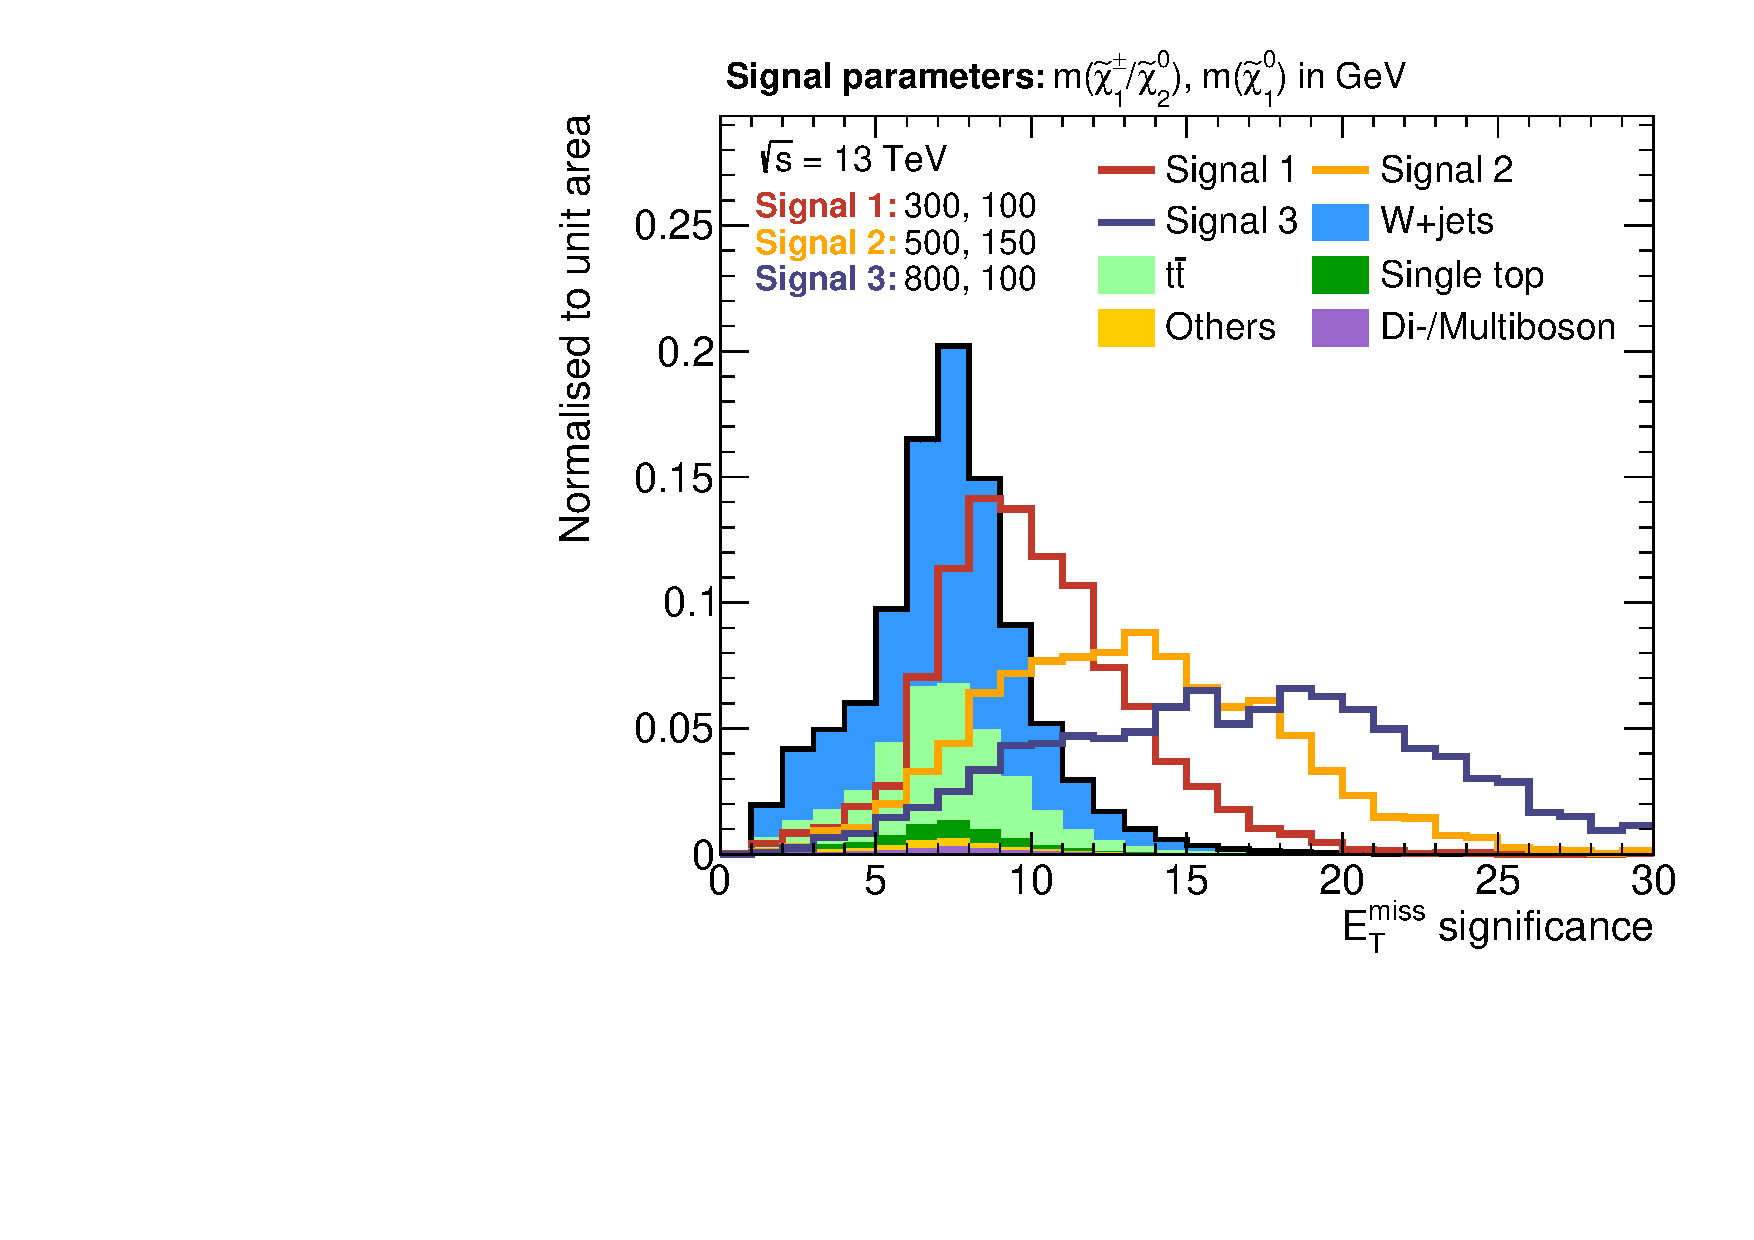
\includegraphics[width=0.8\textwidth]{presel/metsig}
	\end{subfigure}
	\caption{Distributions of the additional observables used during the signal region optimisation. The simulated \gls{sm} backgrounds are stacked on top of each other, and distributions from representative signal models with the quoted mass parameters are overlaid. In order to emphasise the shape differences, both total background and signal distributions are normalised to unity. A preselection of a lepton (electron or muon), at least two jets and $\etmiss > \SI{100}{\GeV}$ is applied.}\label{fig:additional_presel_plots}
\end{figure}

\section{Signal region optimisation}\label{app:n-1_plots_cut_opt}

\graphicspath{{chapter-optimisation/Figs/Vector/}{chapter-optimisation/Figs/}}

\subsection{Raw results from \textit{N}-dimensional scan}

\Cref{fig:additional_presel_plots} shows preselection plots of the additional kinematic observables used during the \textit{N}-dimensional cut scan in \cref{ch:signal_region_optimisation}.

\Cref{fig:results_z_vs_eff_rest} illustrates the results of the $N$-dimensional cut scan for all benchmark signal points considered. As in \cref{ch:signal_region_optimisation}, three different uncertainty configurations are used for computing the significance $Z_\mathrm{B}$, and all values are computed for the two statistically independent subsets of the \gls{mc} datasets used during the $N$-dimensional scan. This approach allows to gauge the impact of statistical fluctuations on the cut combinations tested.

By choosing a well-performing cut combination for each benchmark point, the optimised selections in~\cref{fig:results_n1_800_0,fig:results_n1_800_150,fig:results_n1_800_250,fig:results_n1_600_300,fig:results_n1_400_200,fig:results_n1_300_150} are found after a round of $N$--1 plots. As discussed in~\cref{sec:towards_signal_regions} the optimal cut combinations for each benchmark point are consolidated into multiple \glspl{sr} designed to be sensitive to different kinematic regions of the model parameter space. 

\begin{figure}[hb]
	\centering
	\begin{subfigure}[b]{0.5\linewidth}
		\centering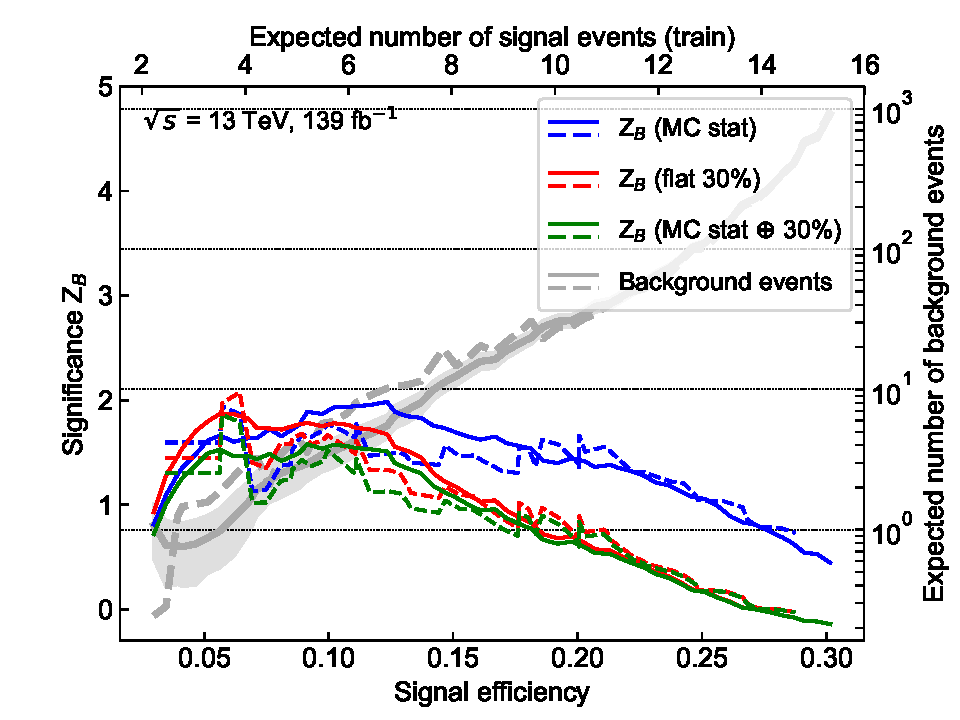
\includegraphics[width=1.0\textwidth]{N-1_cut_scan/z_vs_effs_800_250.pdf}
		\caption{$m(\charg/\neutr), m(\lsp) =  800, \SI{250}{\GeV}$}
	\end{subfigure}\hfill
	\begin{subfigure}[b]{0.5\linewidth}
		\centering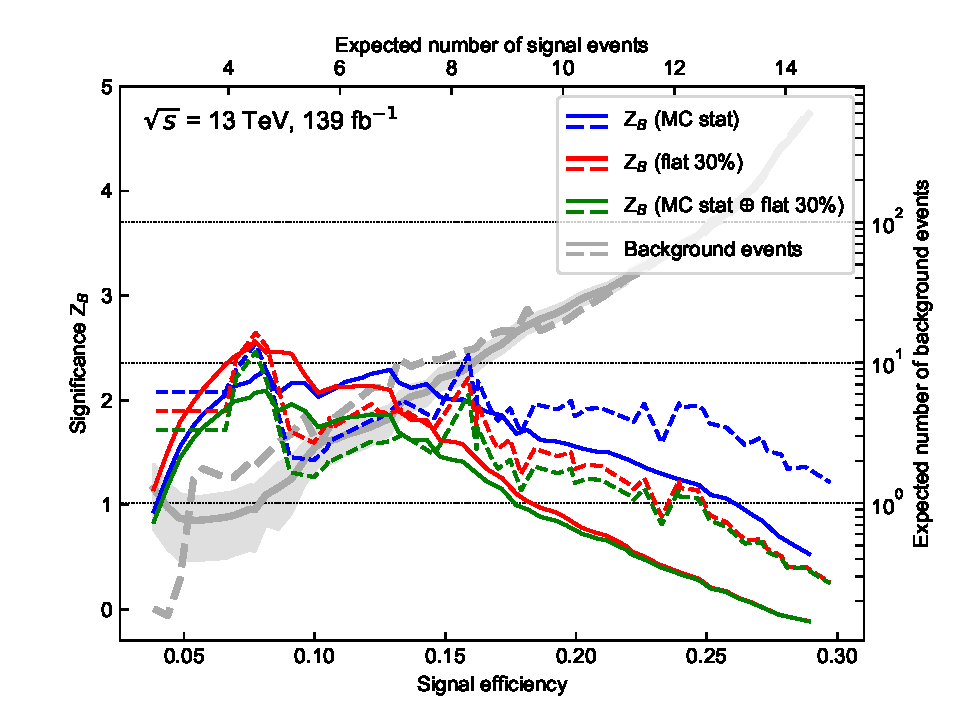
\includegraphics[width=1.0\textwidth]{N-1_cut_scan/z_vs_effs_800_150.pdf}
		\caption{$m(\charg/\neutr), m(\lsp) =  800, \SI{150}{\GeV}$}
	\end{subfigure}\hfill
	\par\bigskip
	\begin{subfigure}[b]{0.5\linewidth}
		\centering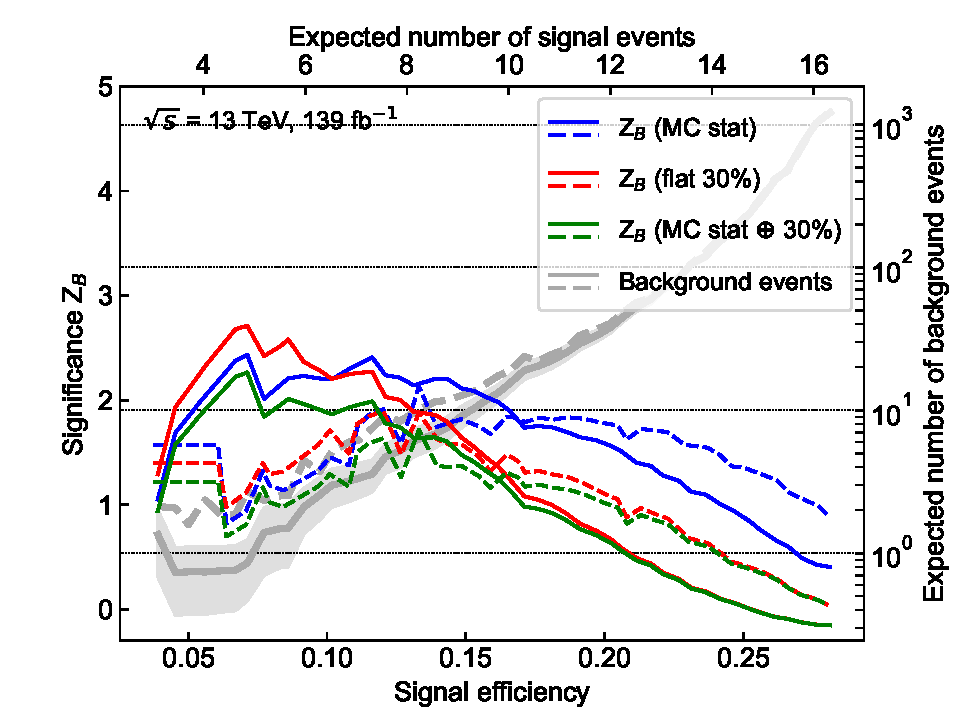
\includegraphics[width=1.0\textwidth]{N-1_cut_scan/z_vs_effs_800_0.pdf}
		\caption{$m(\charg/\neutr), m(\lsp) =  800, \SI{0}{\GeV}$}
	\end{subfigure}\hfill
	\begin{subfigure}[b]{0.5\linewidth}
		\centering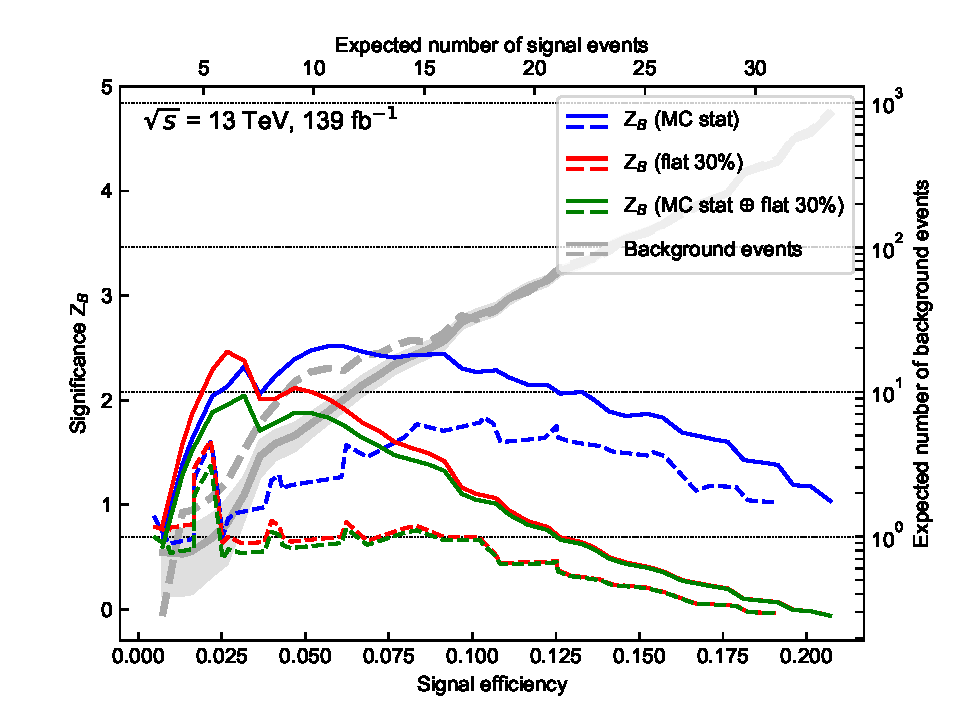
\includegraphics[width=1.0\textwidth]{N-1_cut_scan/z_vs_effs_600_300.pdf}
		\caption{$m(\charg/\neutr), m(\lsp) =  600, \SI{300}{\GeV}$}
	\end{subfigure}\hfill
	\par\bigskip
	\begin{subfigure}[b]{0.5\linewidth}
		\centering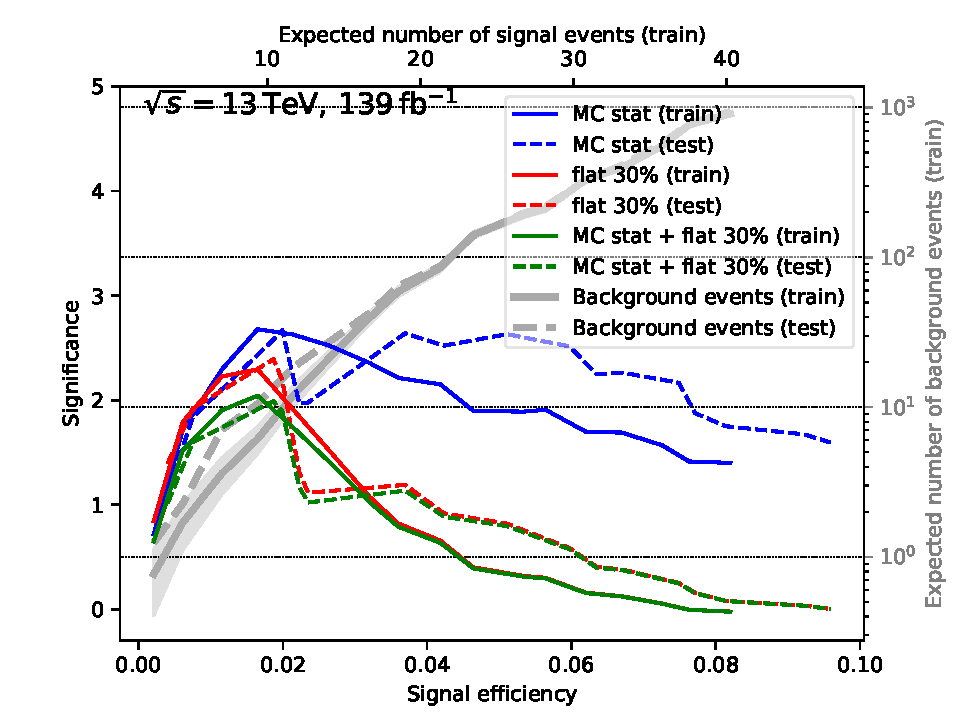
\includegraphics[width=1.0\textwidth]{N-1_cut_scan/z_vs_effs_400_200.pdf}
		\caption{$m(\charg/\neutr), m(\lsp) =  400, \SI{200}{\GeV}$}
	\end{subfigure}\hfill
	\begin{subfigure}[b]{0.5\linewidth}
		\centering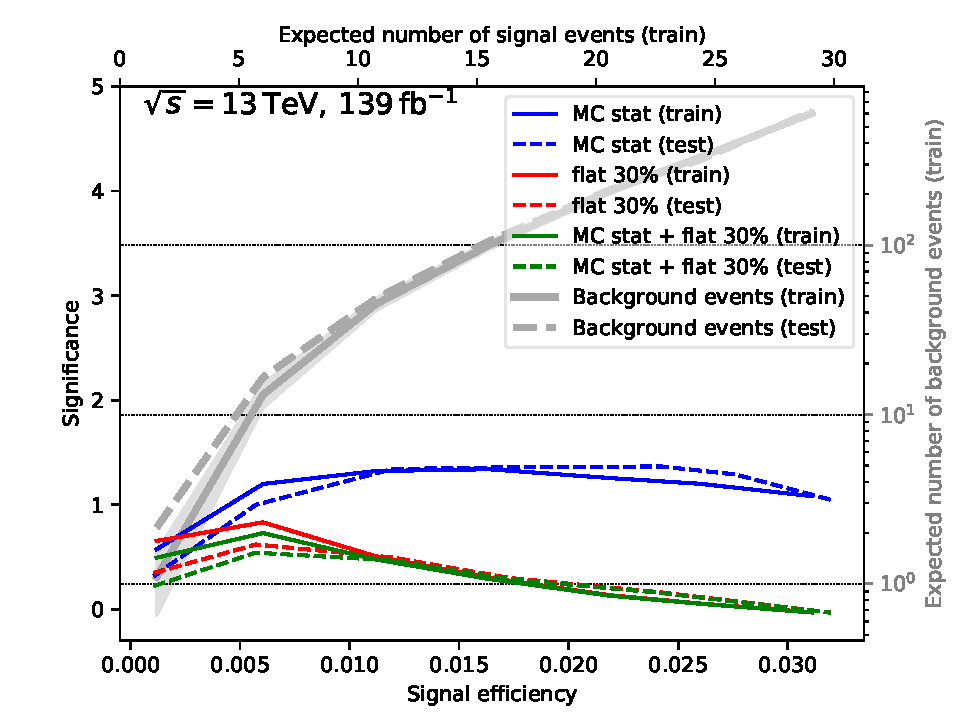
\includegraphics[width=1.0\textwidth]{N-1_cut_scan/z_vs_effs_300_150.pdf}
		\caption{$m(\charg/\neutr), m(\lsp) =  300, \SI{150}{\GeV}$}
	\end{subfigure}\hfill

	\caption[N-dimensional cut scan results]{Results of the $N$-dimensional cut scan for all benchmark points. The binomial discovery significance $Z_\mathrm{B}$ is plotted against the signal efficiency for varying uncertainty configurations. Additionally, the expected \gls{sm} background rates are shown, including statistical uncertainties for one of the two statistically independent samples (shaded area). The solid and dashed lines represent the two statistically independent subsets that the \gls{mc} datasets are split into.}
	\label{fig:results_z_vs_eff_rest}
\end{figure}


\begin{figure}
	\centering
	\begin{subfigure}[b]{0.5\linewidth}
		\centering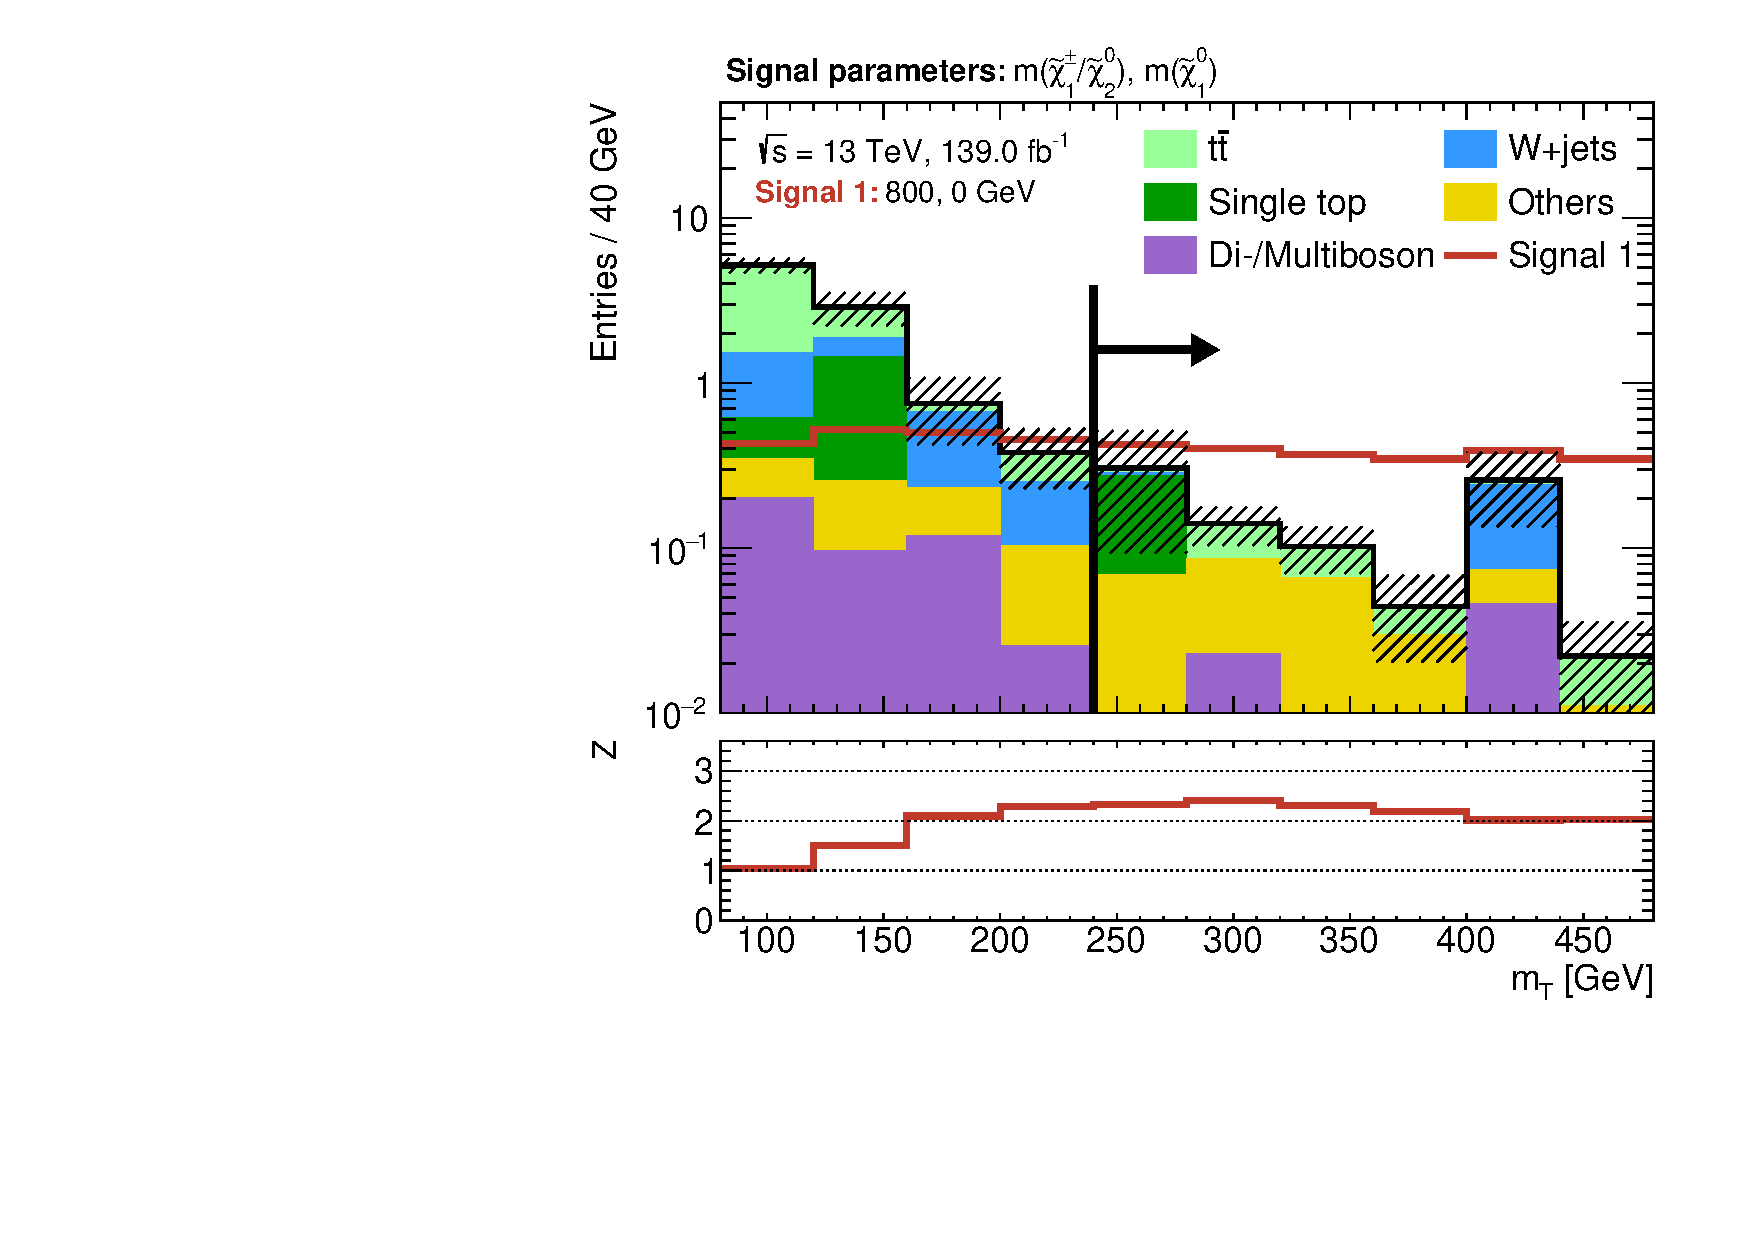
\includegraphics[width=0.9\textwidth]{N-1_cut_scan/n1_800_0/mt}
	\end{subfigure}\hfill
	\begin{subfigure}[b]{0.5\linewidth}
		\centering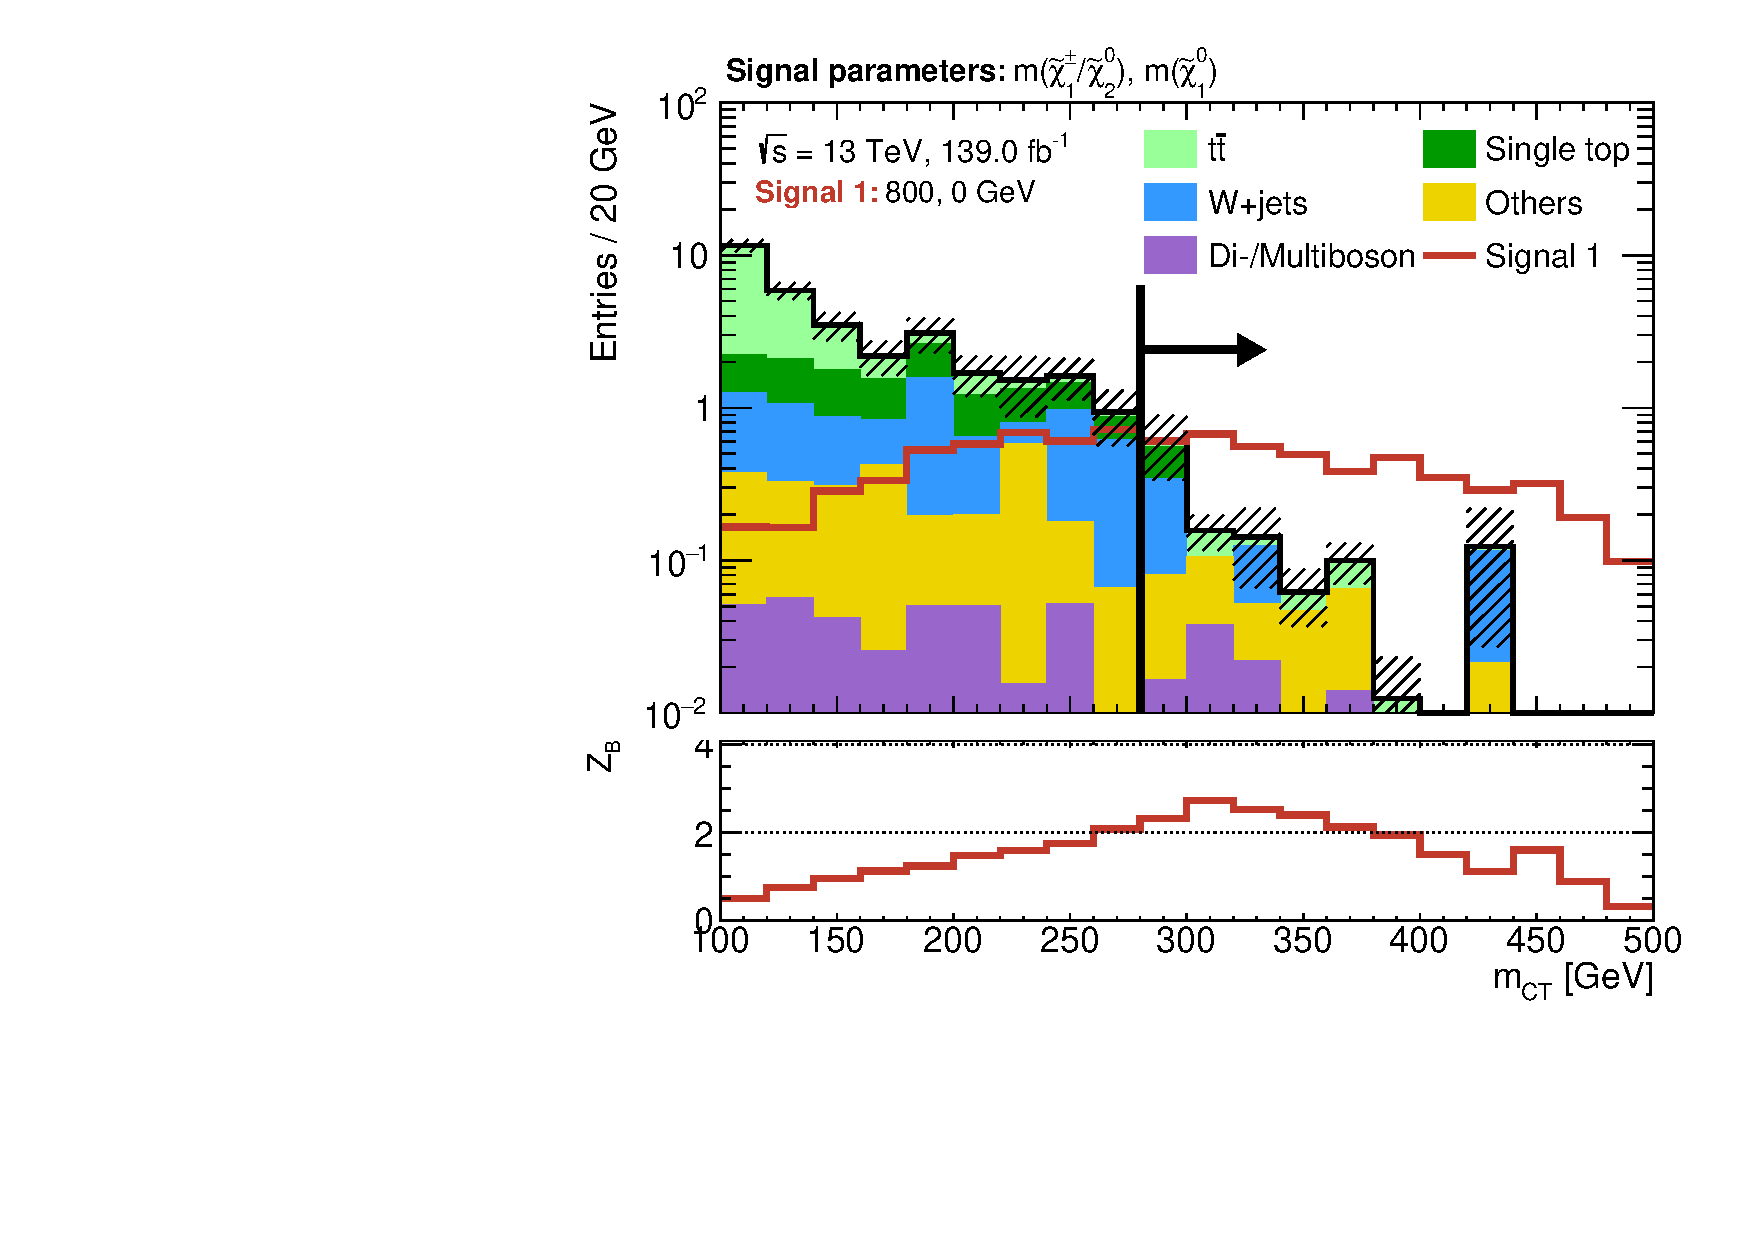
\includegraphics[width=0.9\textwidth]{N-1_cut_scan/n1_800_0/mct}
	\end{subfigure}\hfill
	\par\medskip
	\begin{subfigure}[b]{0.5\linewidth}
		\centering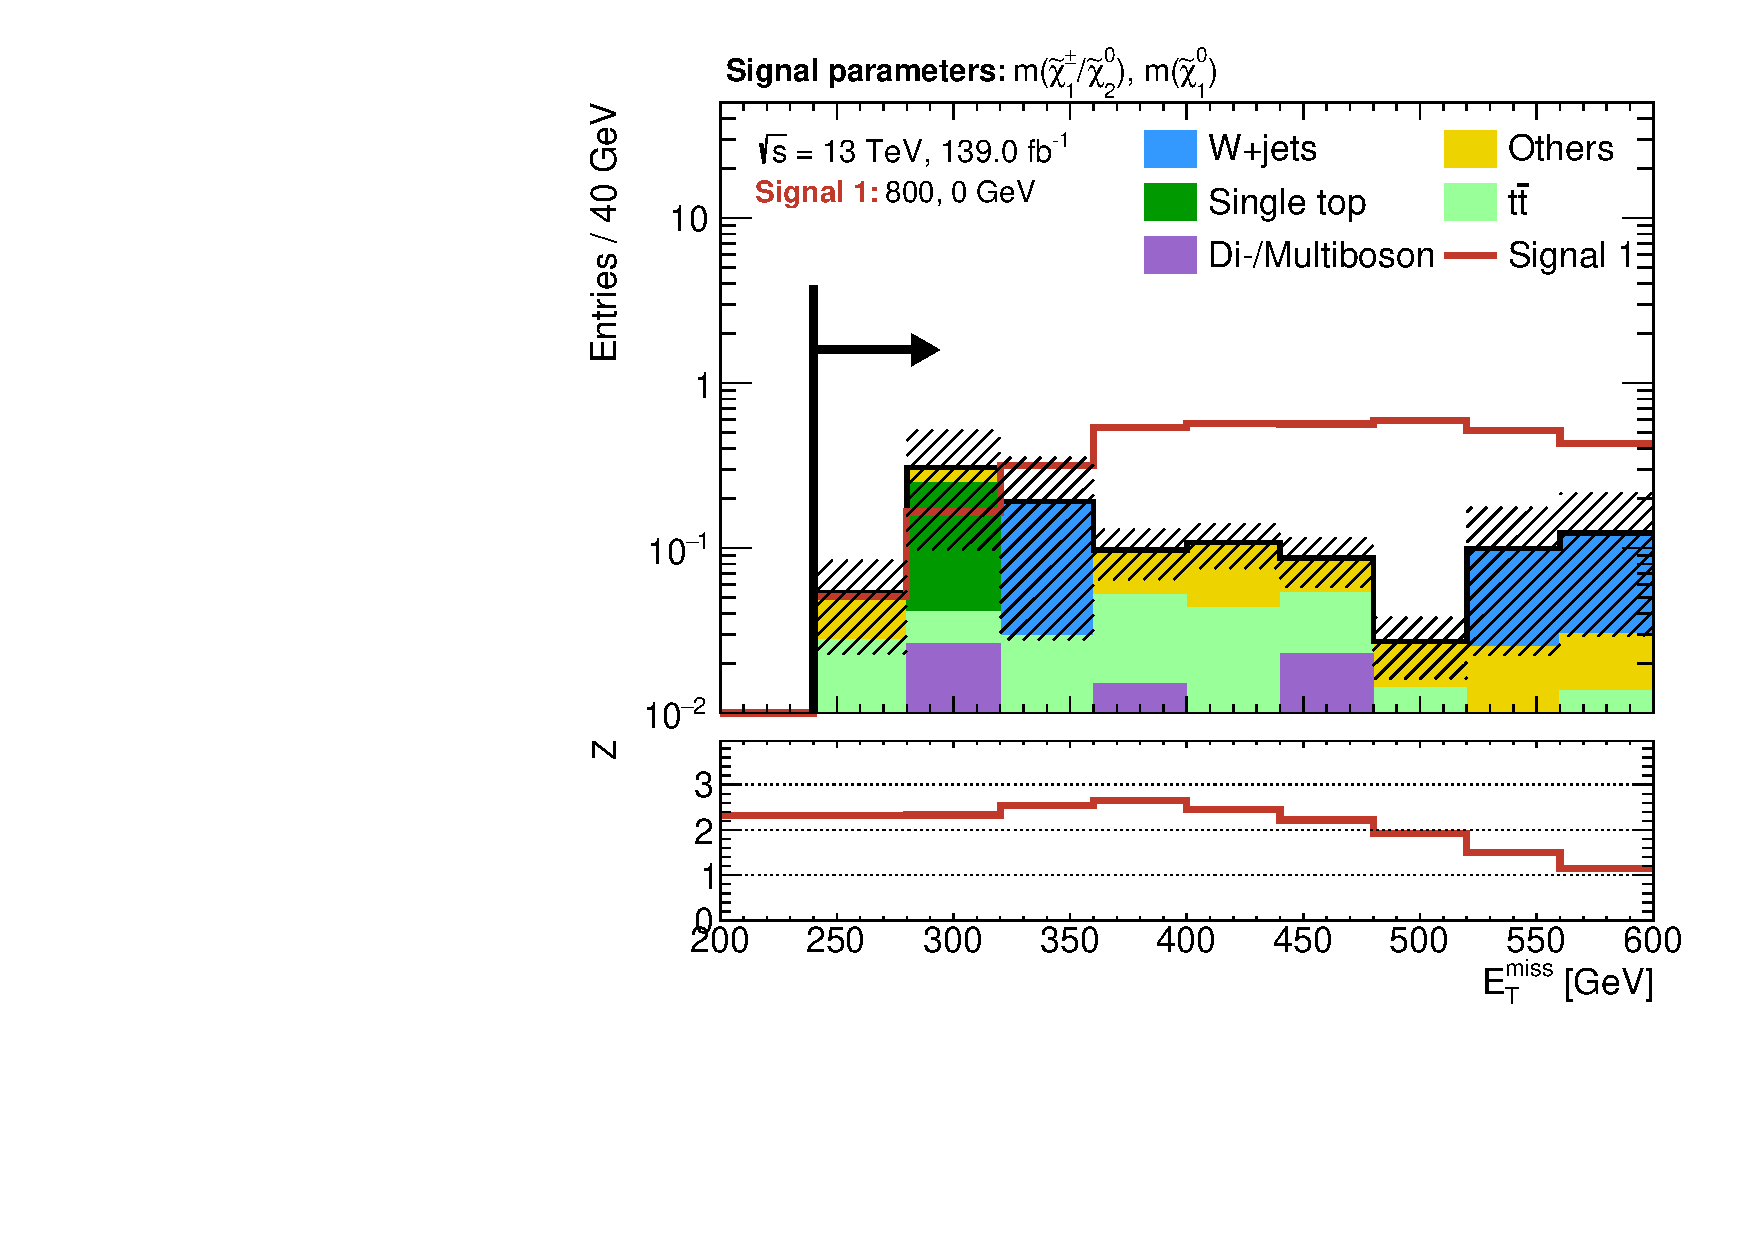
\includegraphics[width=0.9\textwidth]{N-1_cut_scan/n1_800_0/met}
	\end{subfigure}\hfill
	\begin{subfigure}[b]{0.5\linewidth}
		\centering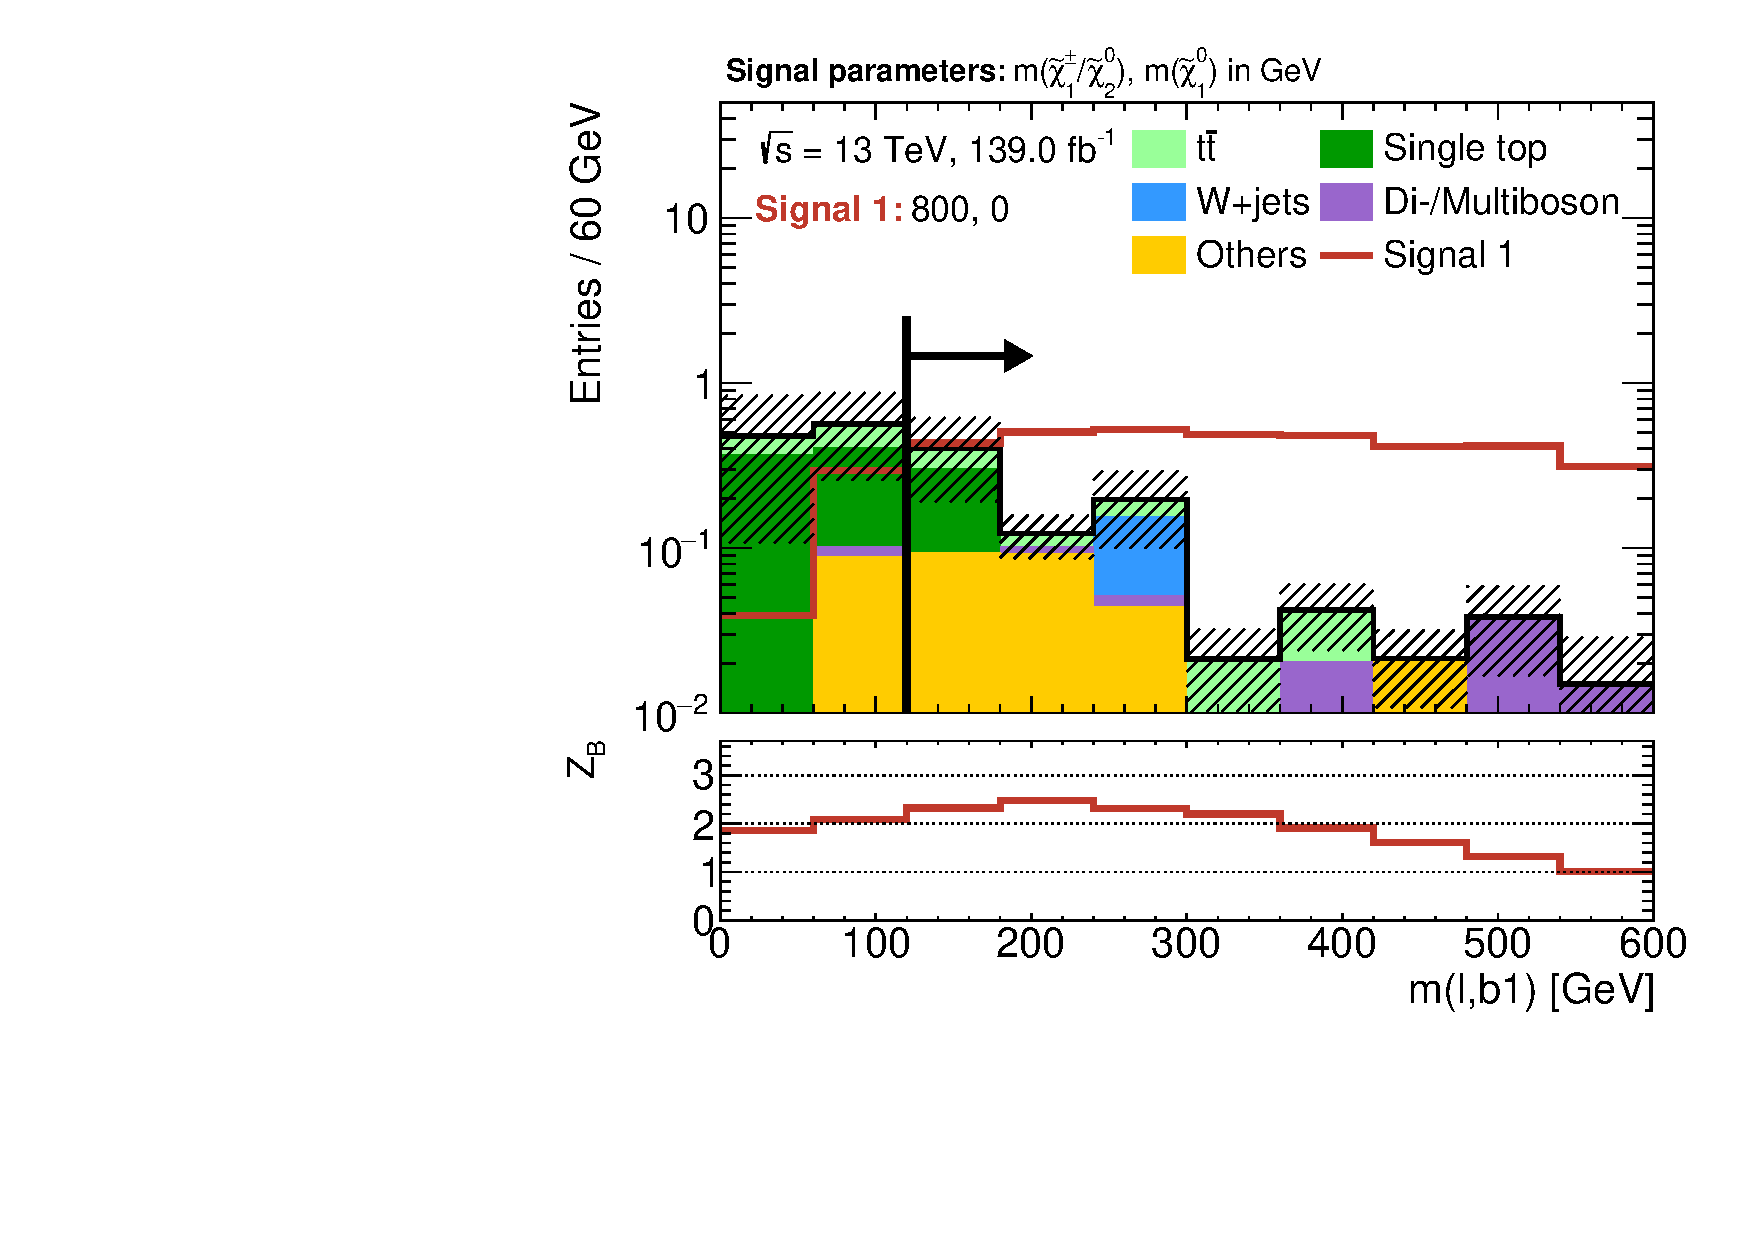
\includegraphics[width=0.9\textwidth]{N-1_cut_scan/n1_800_0/mlb1}
	\end{subfigure}\hfill
	\par\medskip
	\begin{subfigure}[b]{0.5\linewidth}
		\centering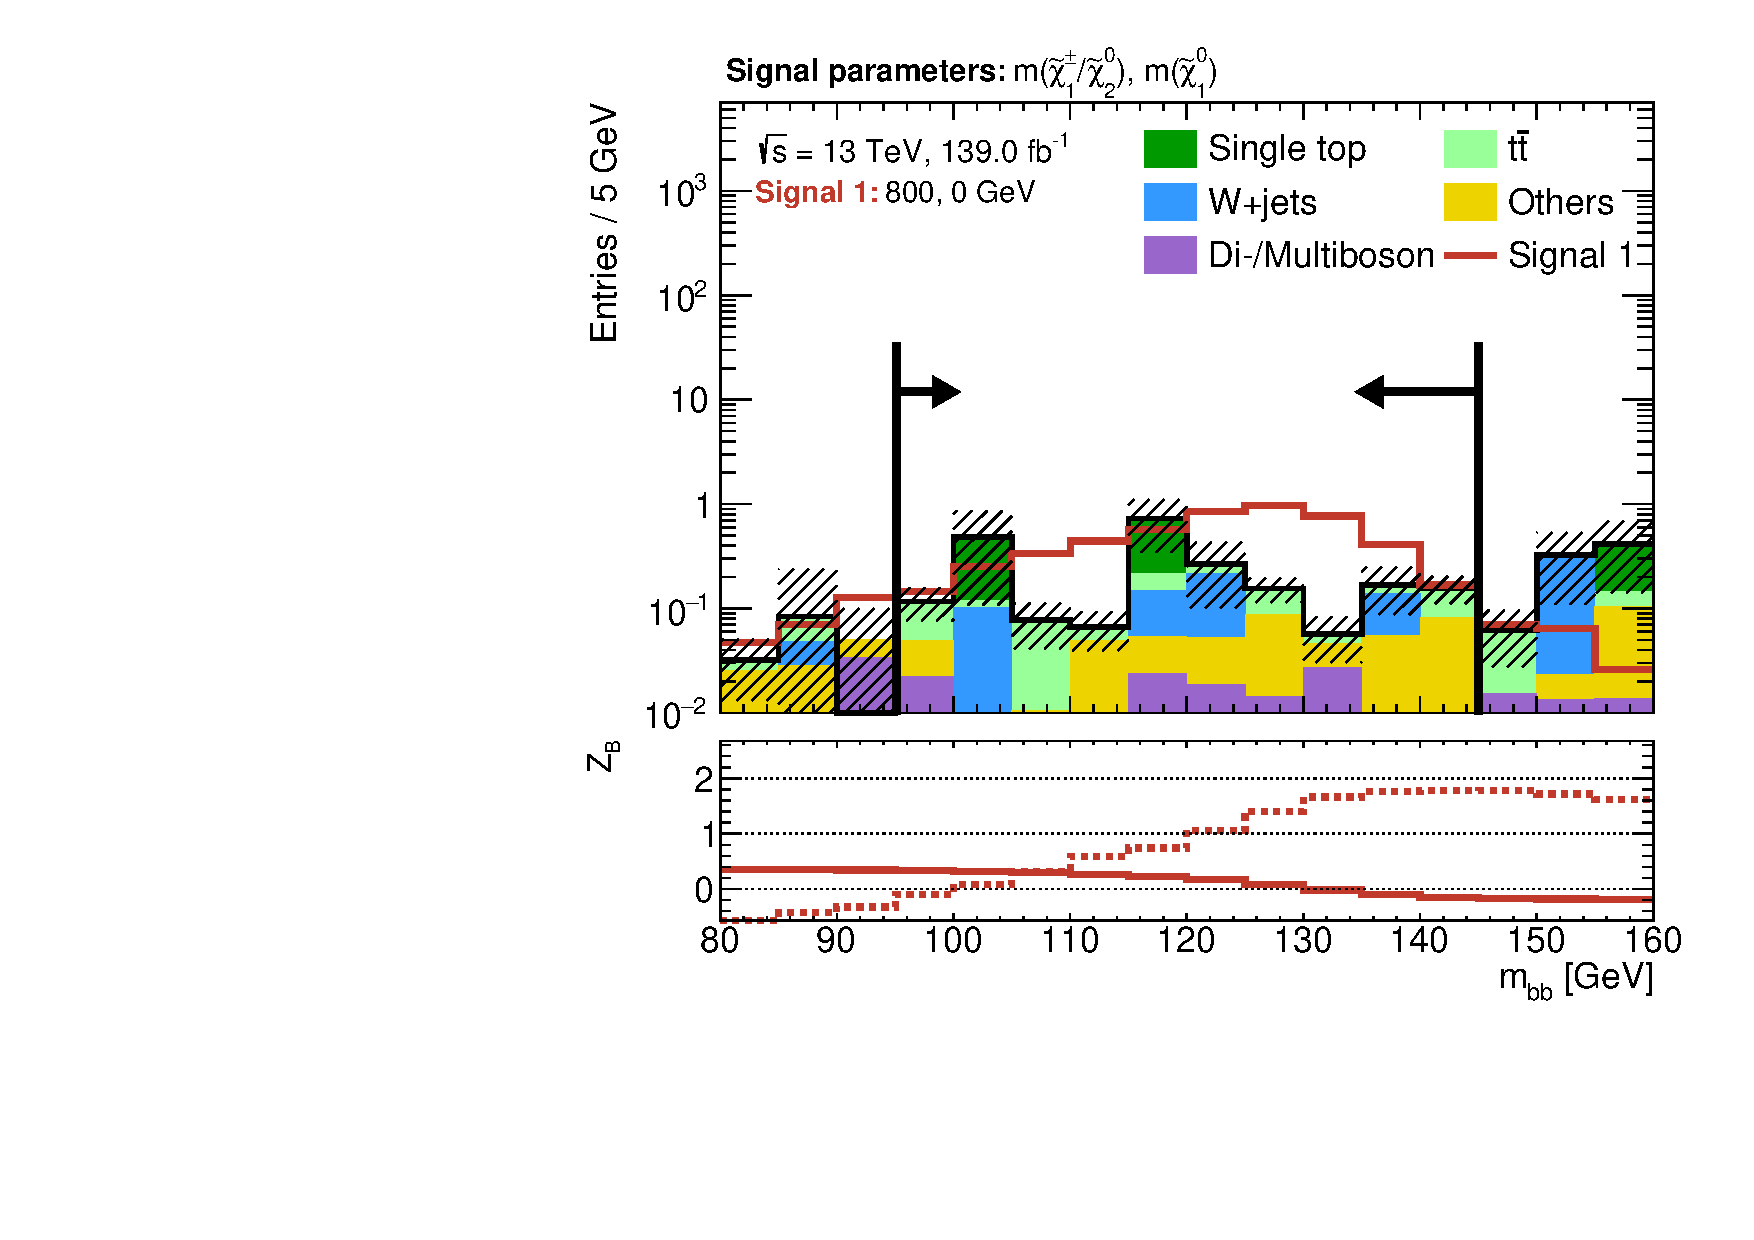
\includegraphics[width=0.9\textwidth]{N-1_cut_scan/n1_800_0/mbb_both}
	\end{subfigure}\hfill
	\begin{subfigure}[b]{0.5\linewidth}
		\centering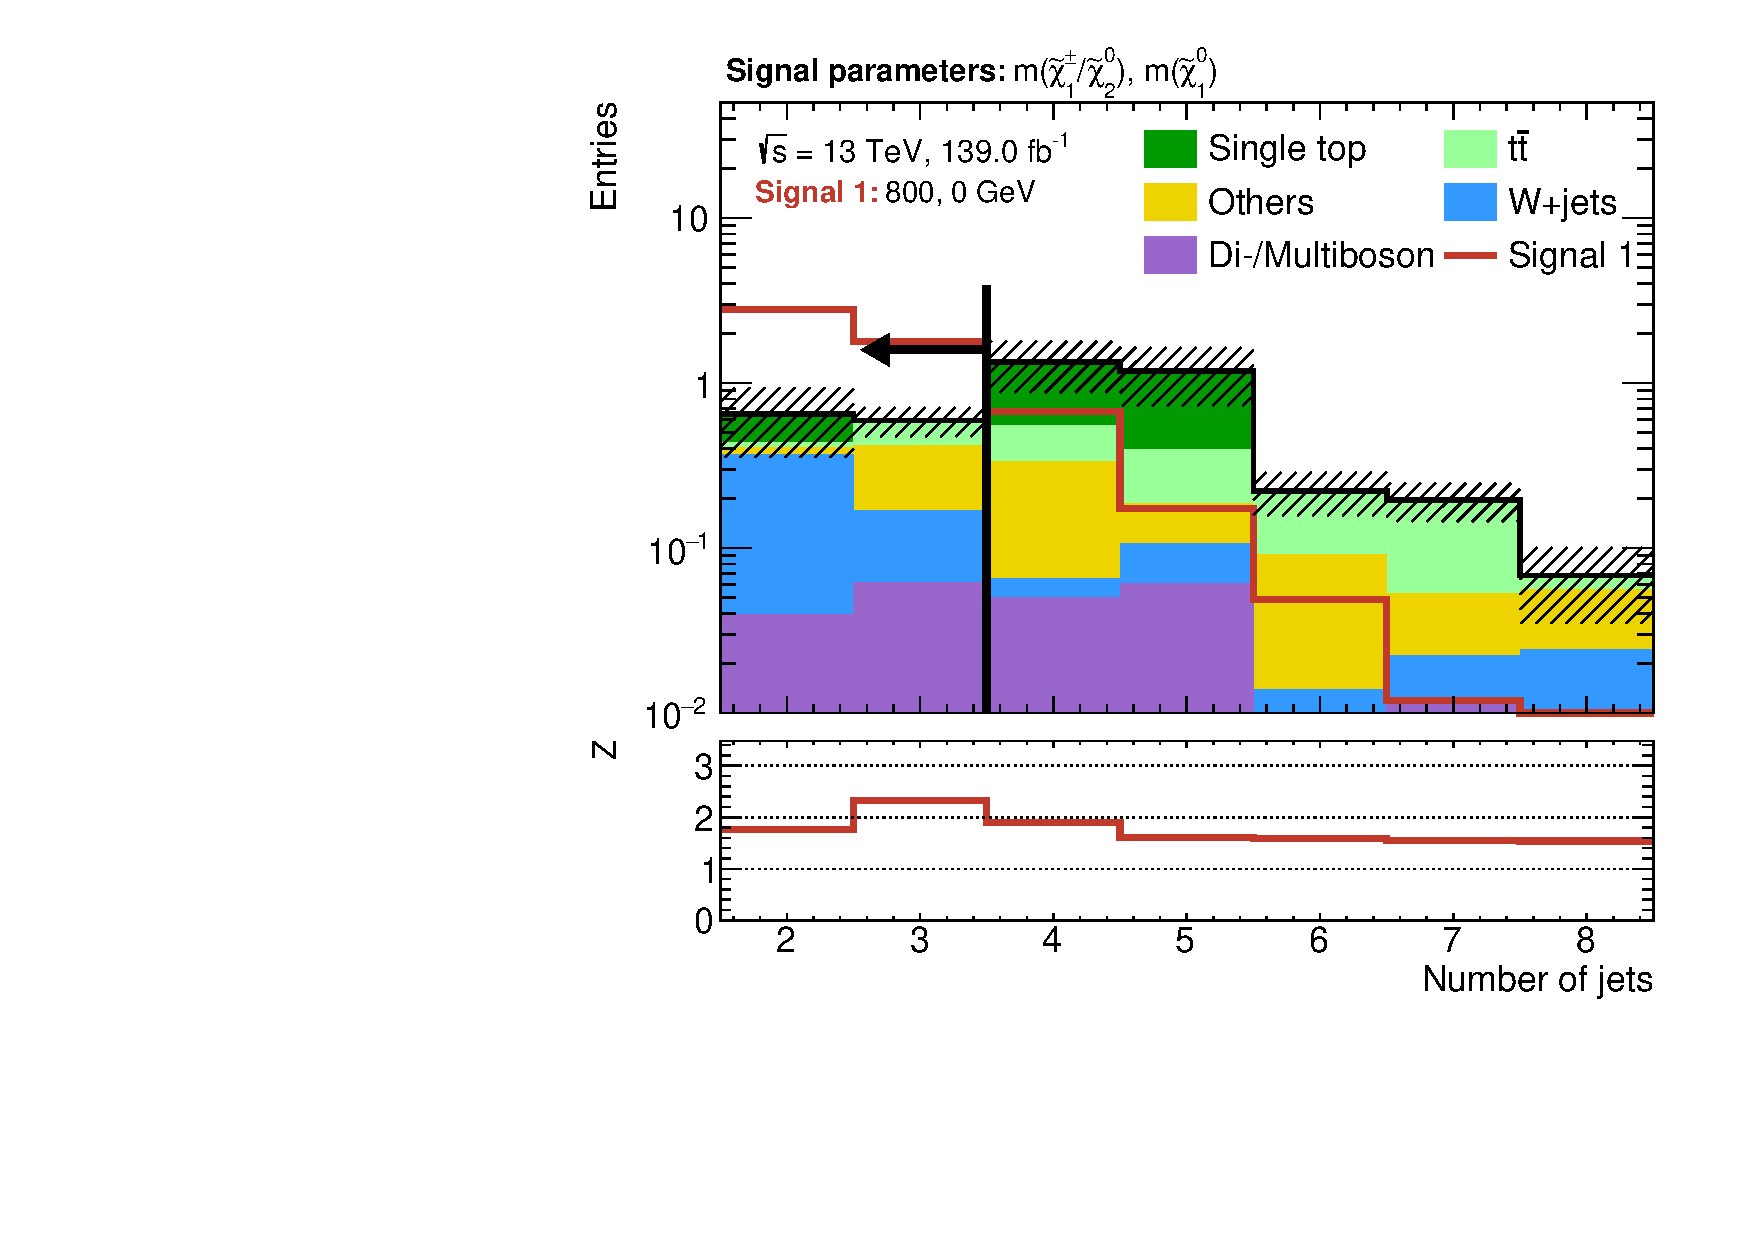
\includegraphics[width=0.9\textwidth]{N-1_cut_scan/n1_800_0/nJet30}
	\end{subfigure}

	\caption[\textit{N}--1 plots for the chosen cut combination for the (800, 0) signal point]{\textit{N}--1 plots for the chosen cut combination for the $(m(\charg/\neutr), m(\lsp)) = (\SI{800}{\GeV}, \SI{0}{\GeV})$ signal point. The shaded region includes \gls{mc} statistical as well as 30\% systematic uncertainties (added in quadrature) on the background. The significance is computed using the binomial discovery significance using the uncertainty on the background.}
	\label{fig:results_n1_800_0}
\end{figure}



\begin{figure}
	\centering
	\begin{subfigure}[b]{0.5\linewidth}
		\centering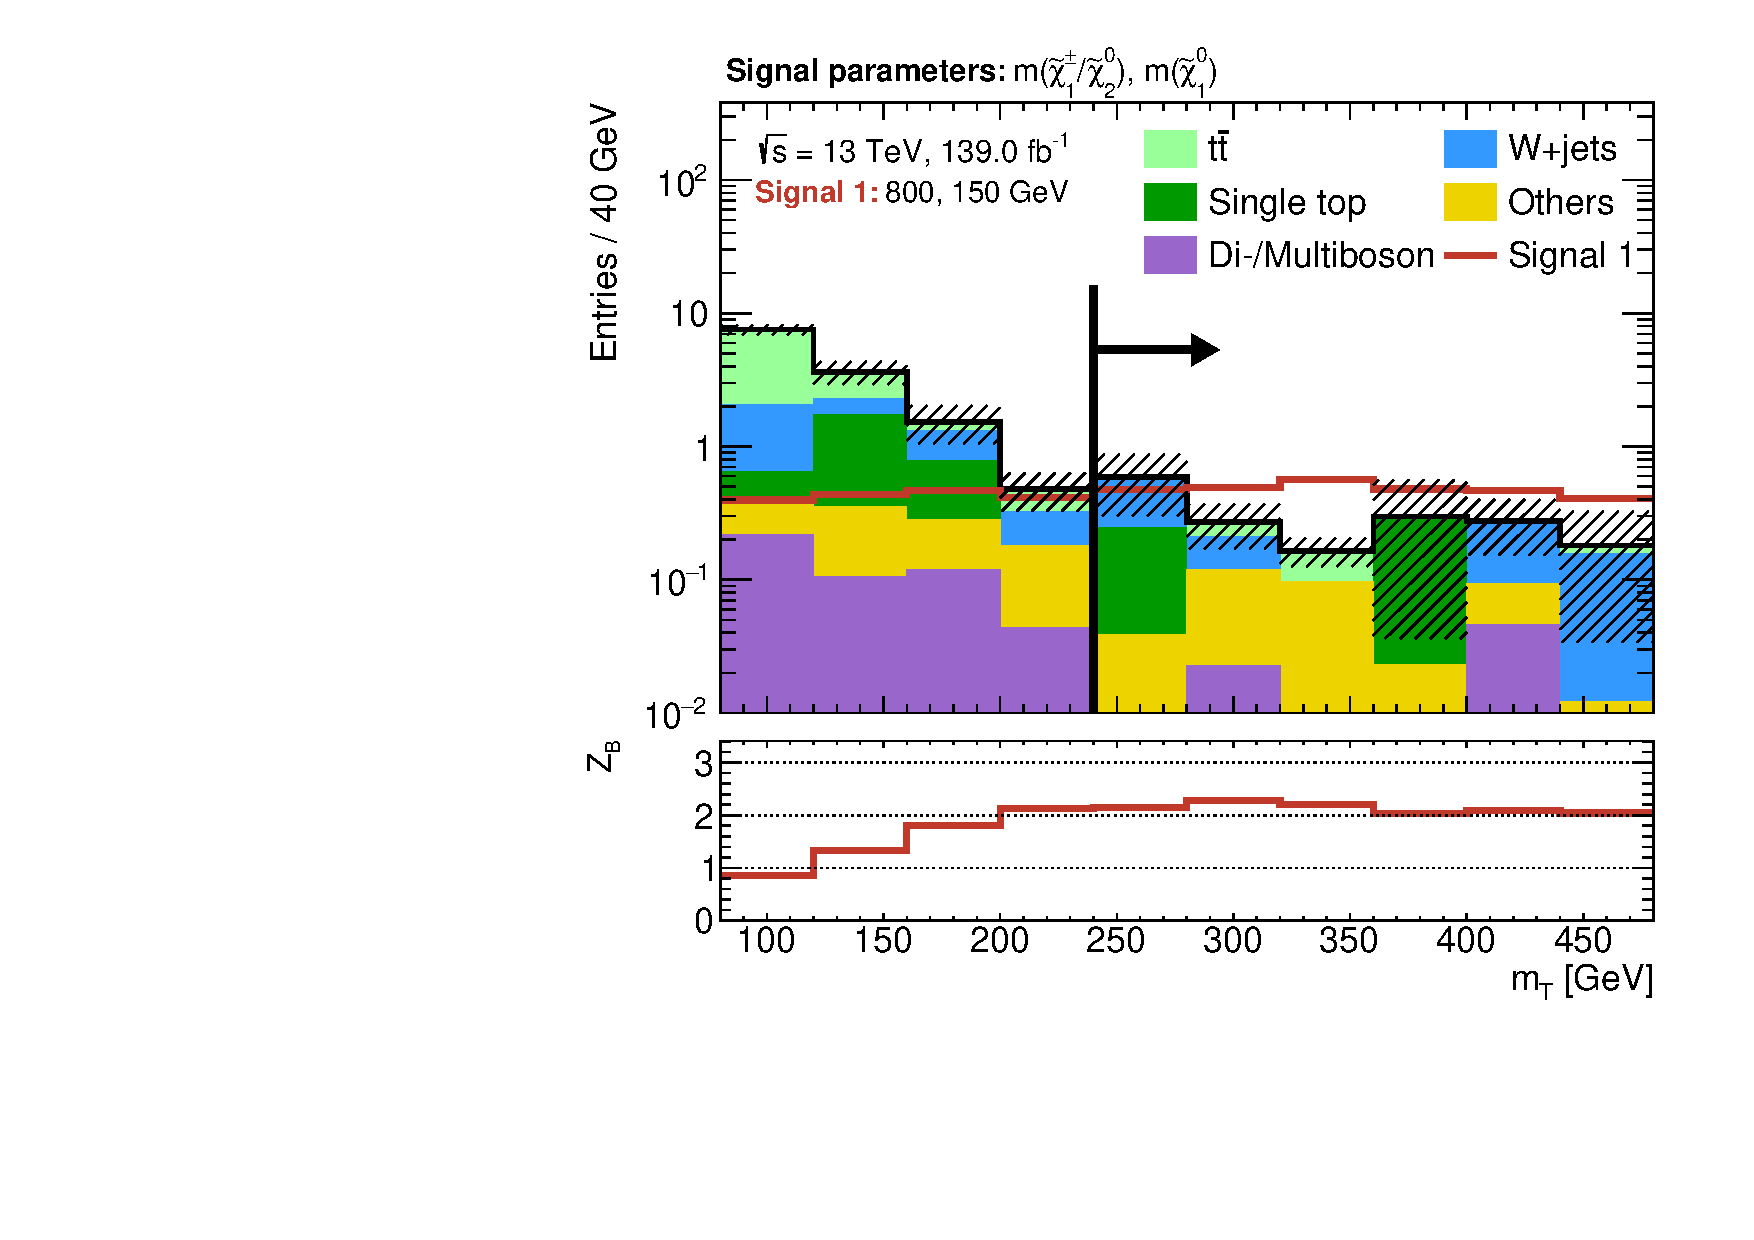
\includegraphics[width=0.9\textwidth]{N-1_cut_scan/n1_800_150/mt}
	\end{subfigure}\hfill
	\begin{subfigure}[b]{0.5\linewidth}
		\centering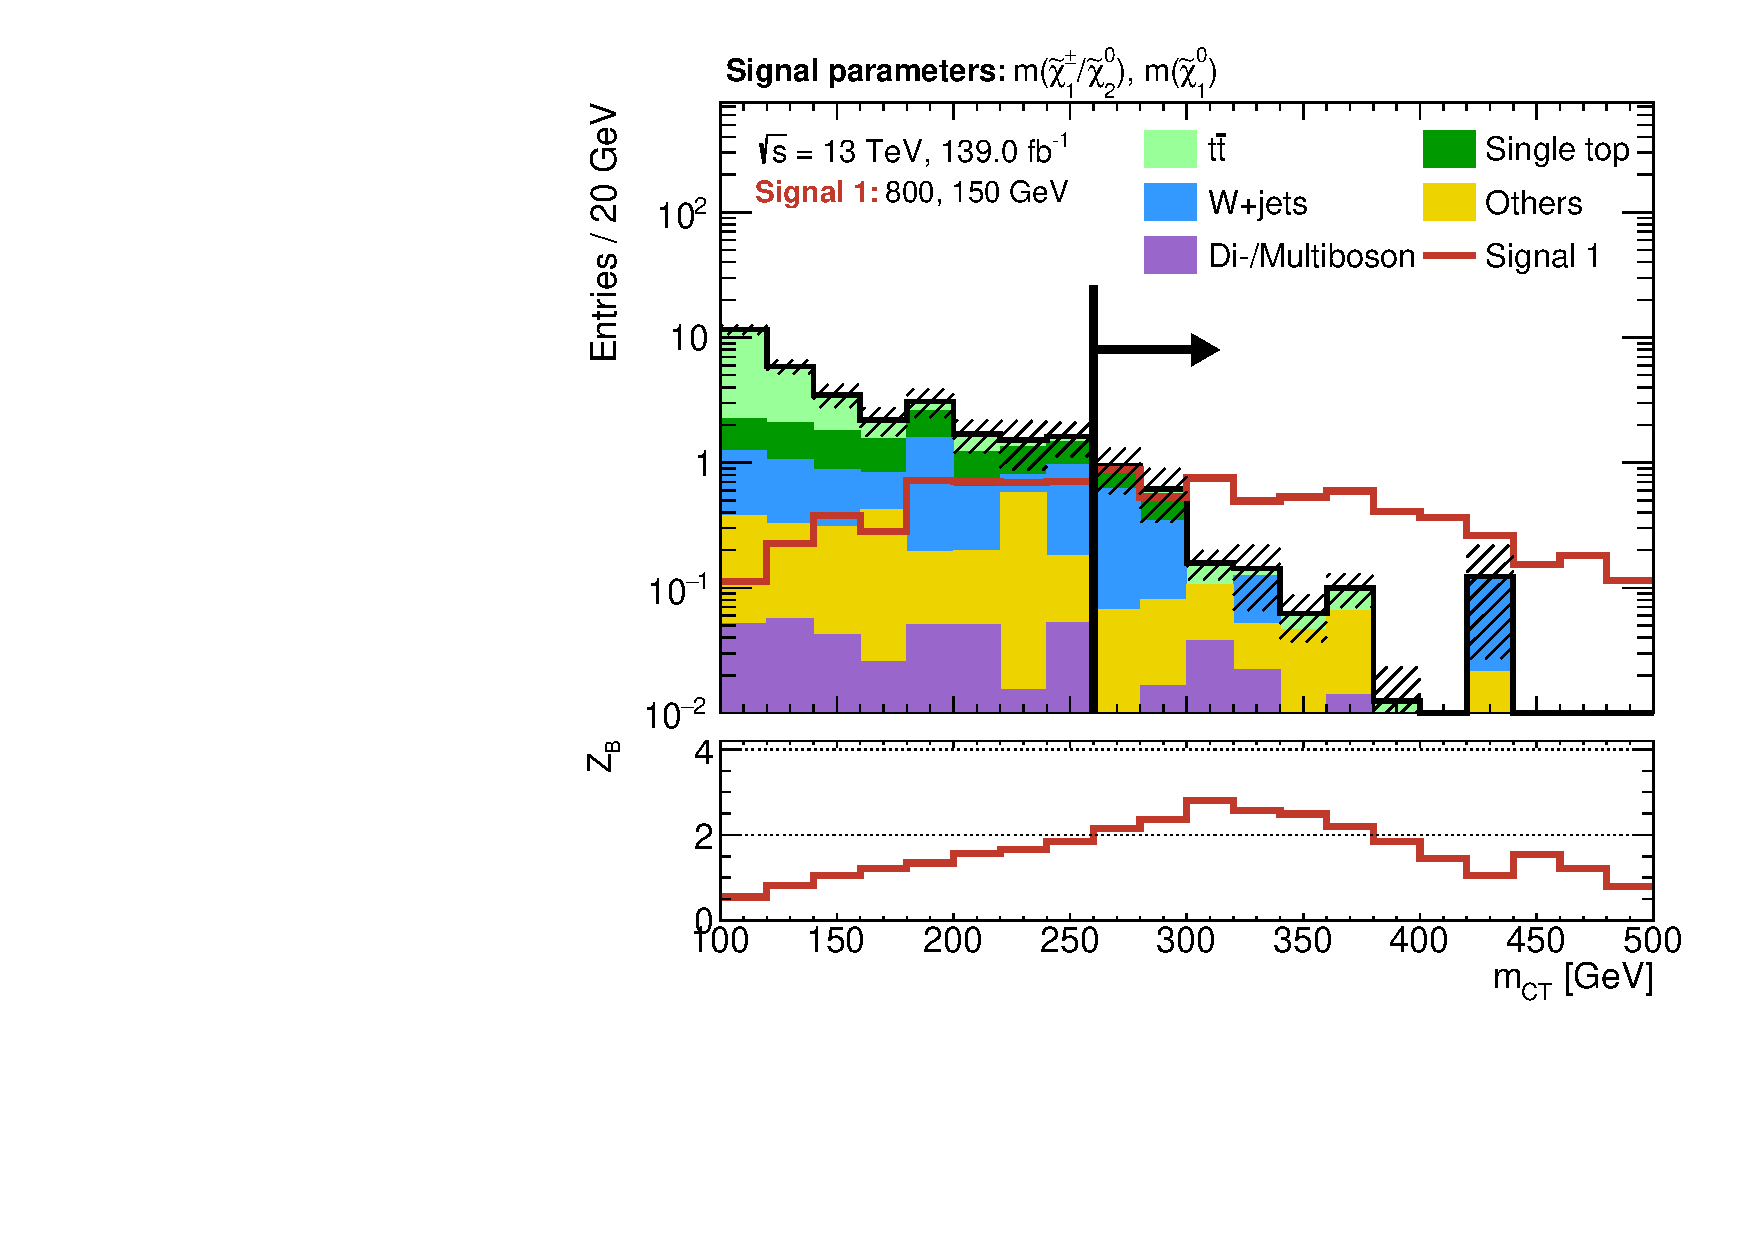
\includegraphics[width=0.9\textwidth]{N-1_cut_scan/n1_800_150/mct}
	\end{subfigure}\hfill
	\begin{subfigure}[b]{0.5\linewidth}
		\centering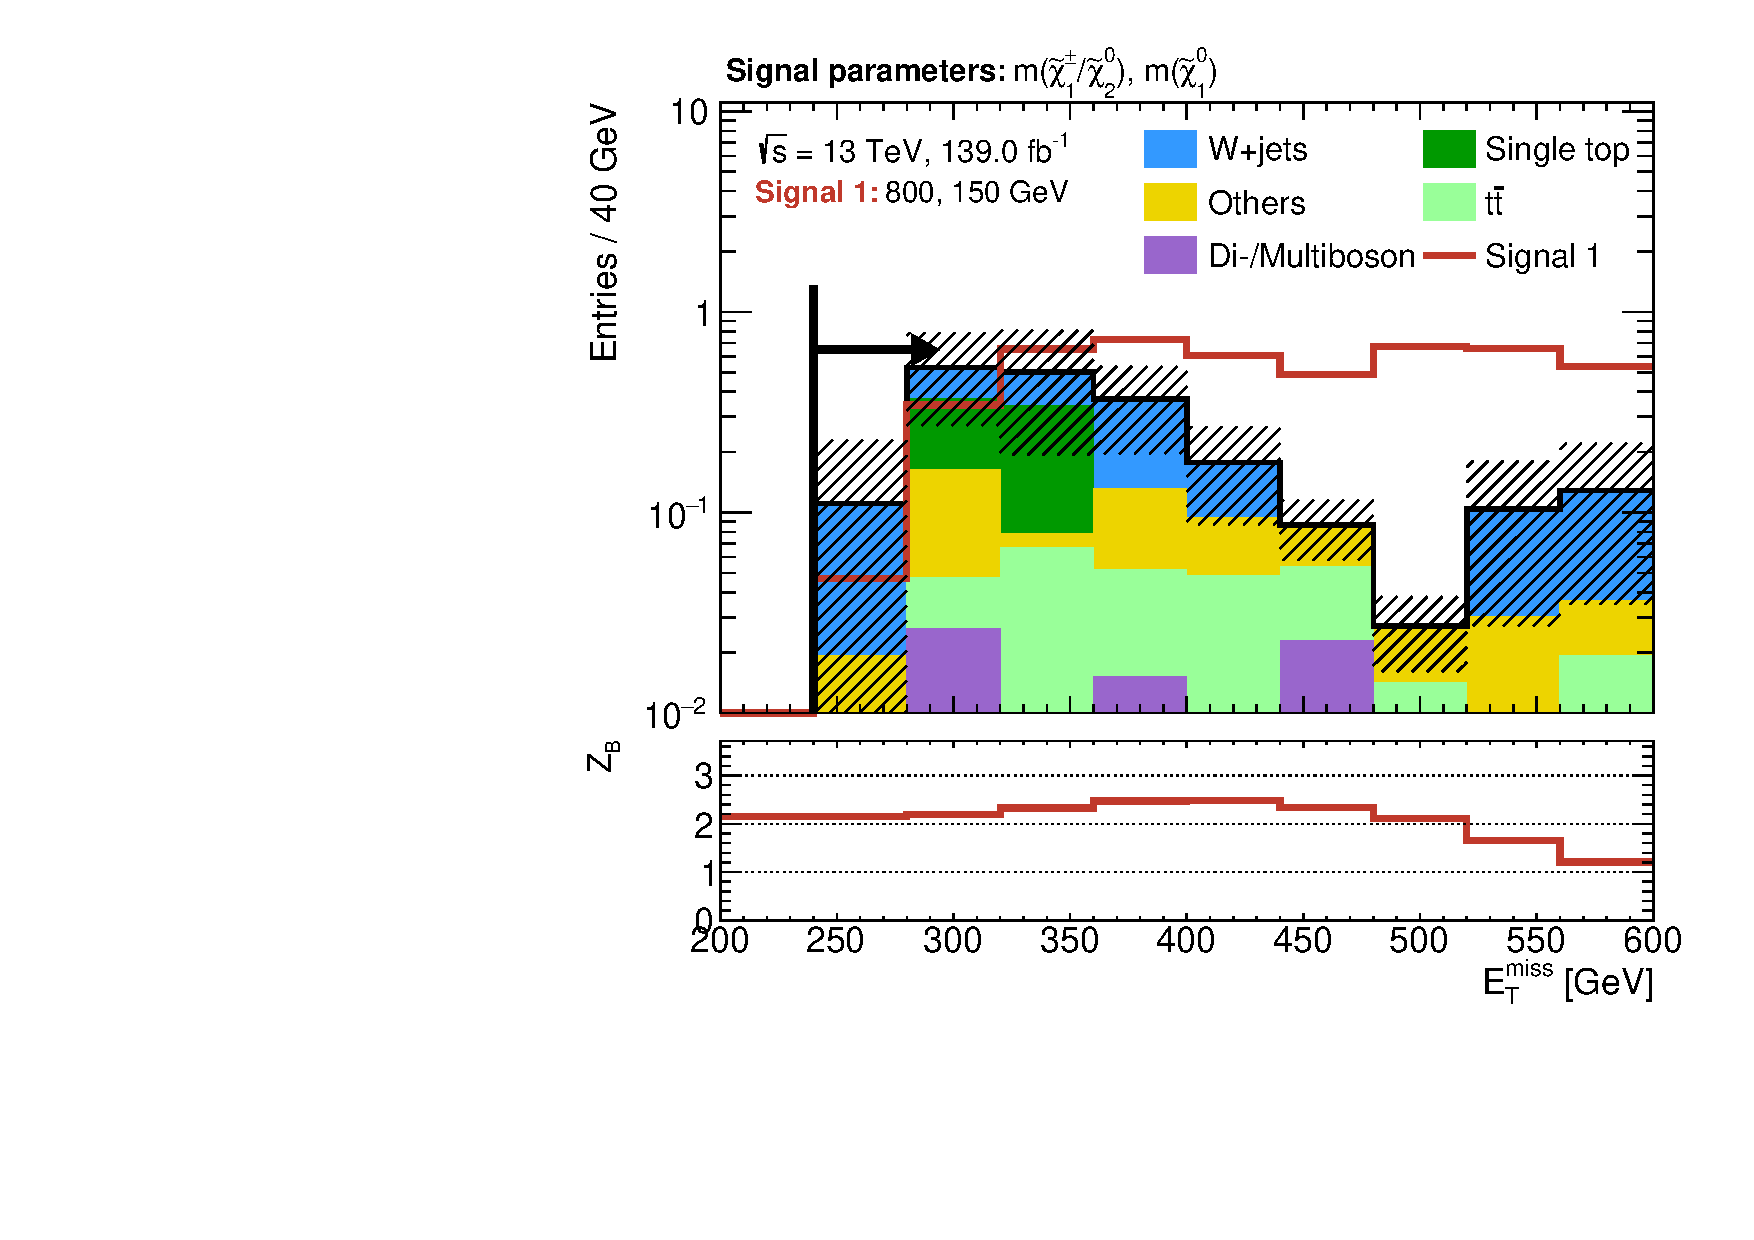
\includegraphics[width=0.9\textwidth]{N-1_cut_scan/n1_800_150/met}
	\end{subfigure}\hfill
	\begin{subfigure}[b]{0.5\linewidth}
		\centering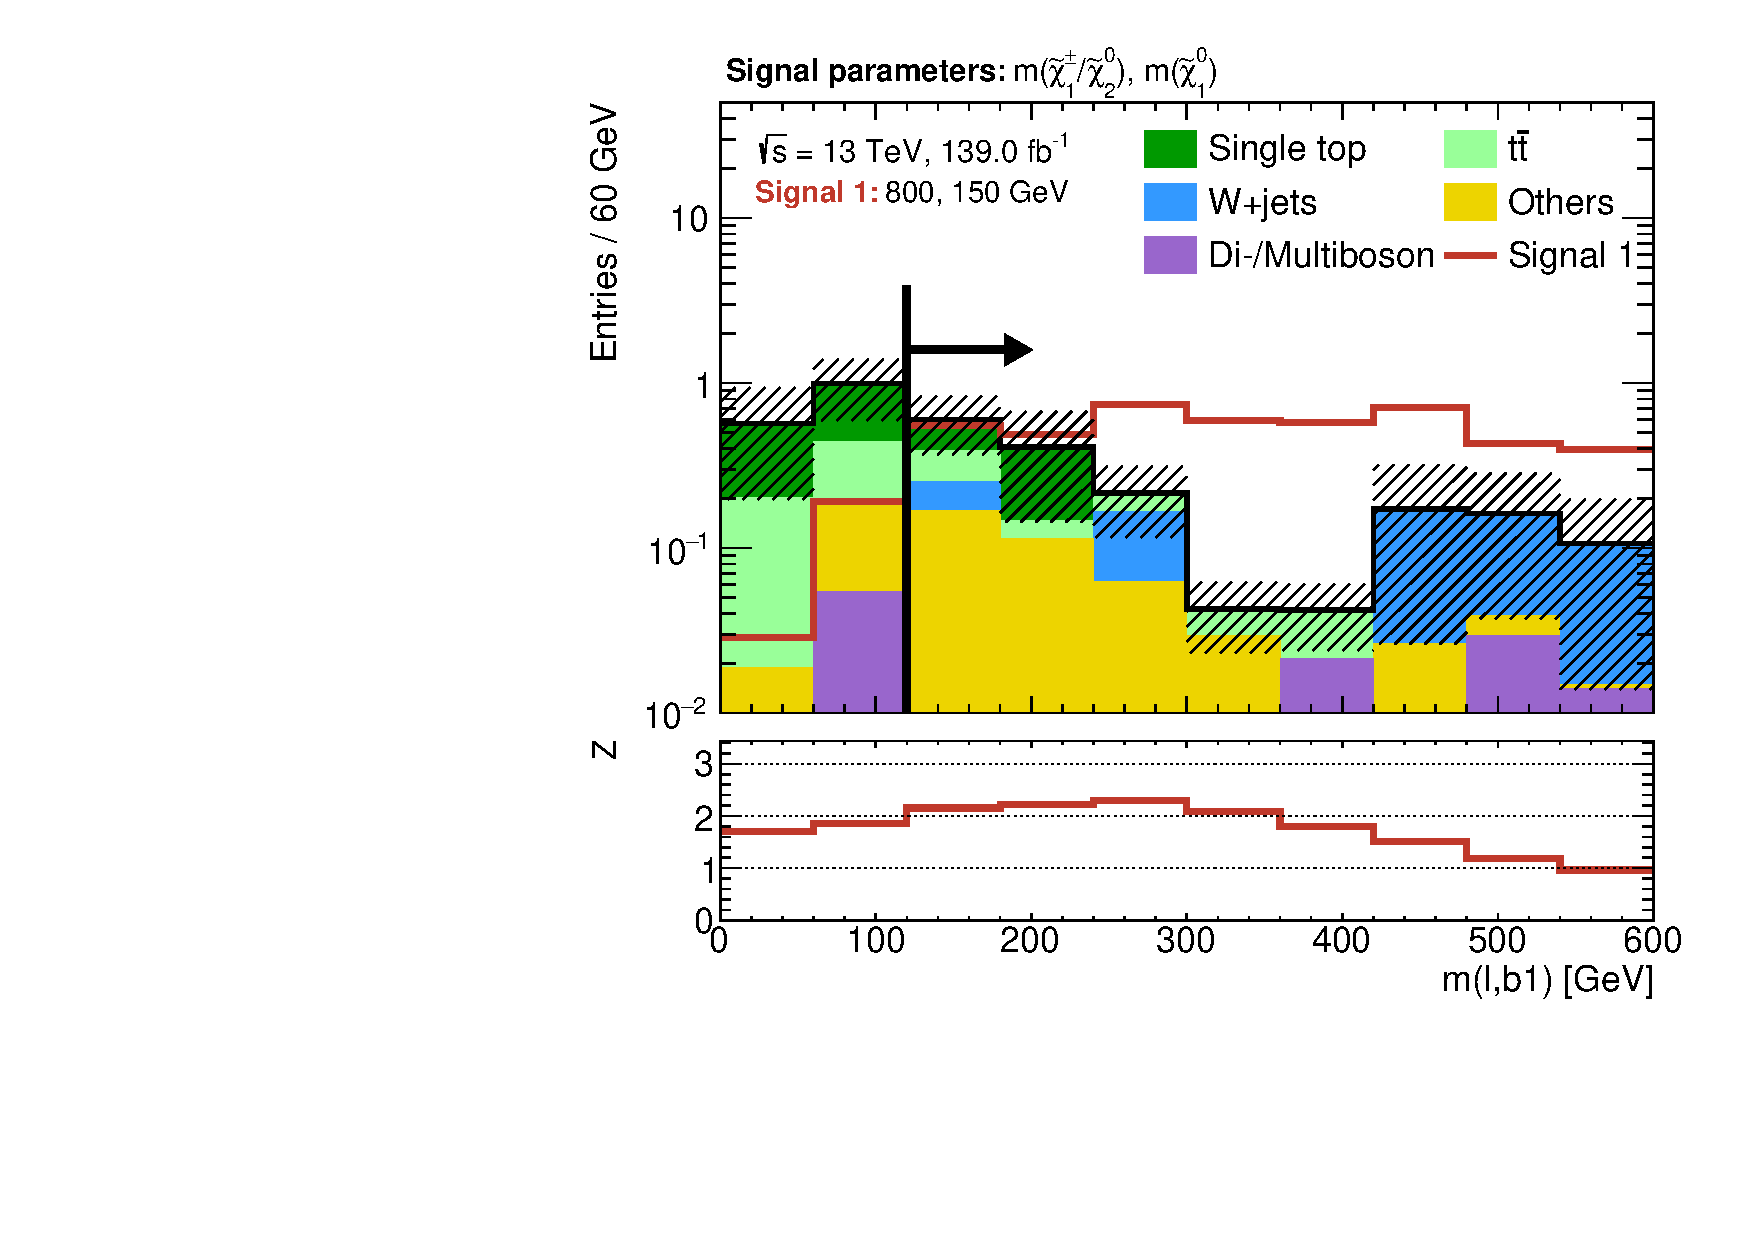
\includegraphics[width=0.9\textwidth]{N-1_cut_scan/n1_800_150/mlb1}
	\end{subfigure}\hfill
	\begin{subfigure}[b]{0.5\linewidth}
		\centering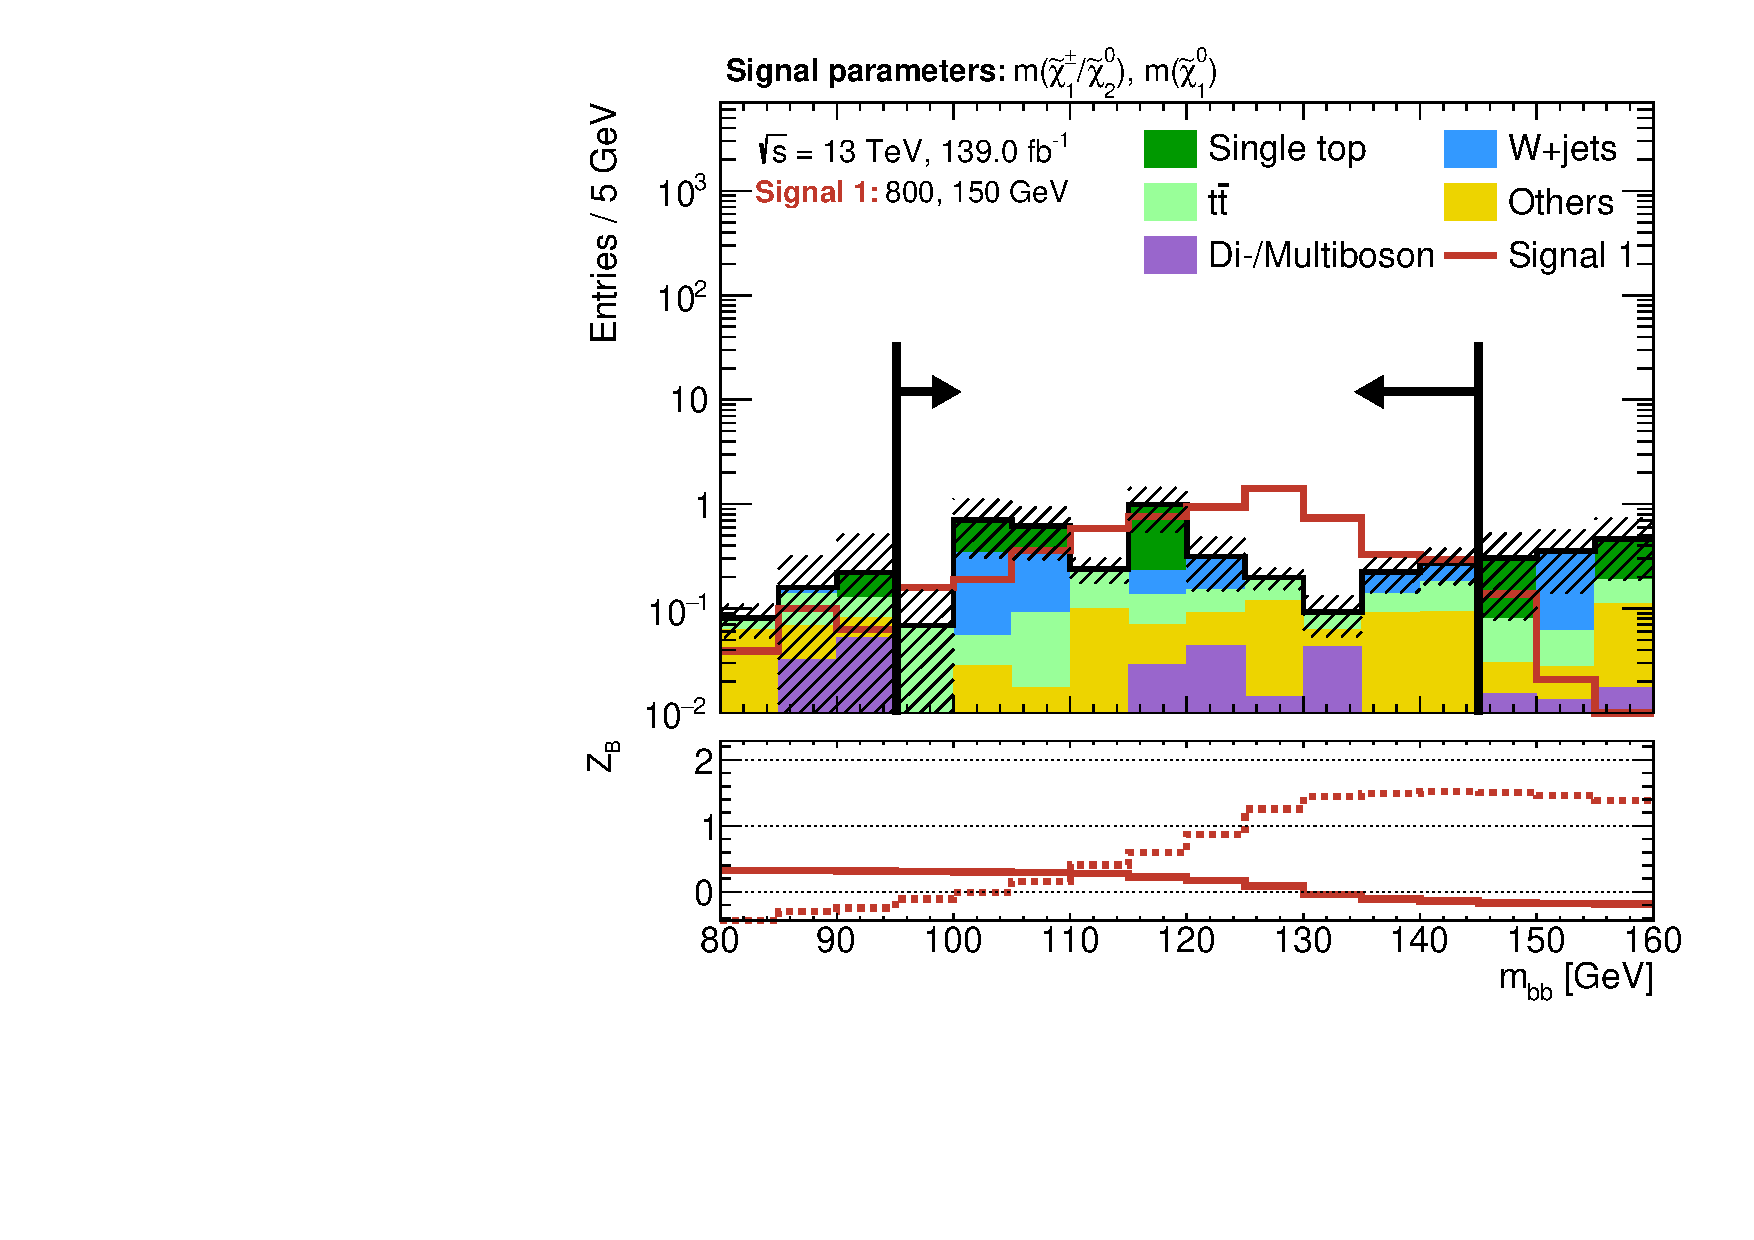
\includegraphics[width=0.9\textwidth]{N-1_cut_scan/n1_800_150/mbb_both}
	\end{subfigure}\hfill
	\begin{subfigure}[b]{0.5\linewidth}
		\centering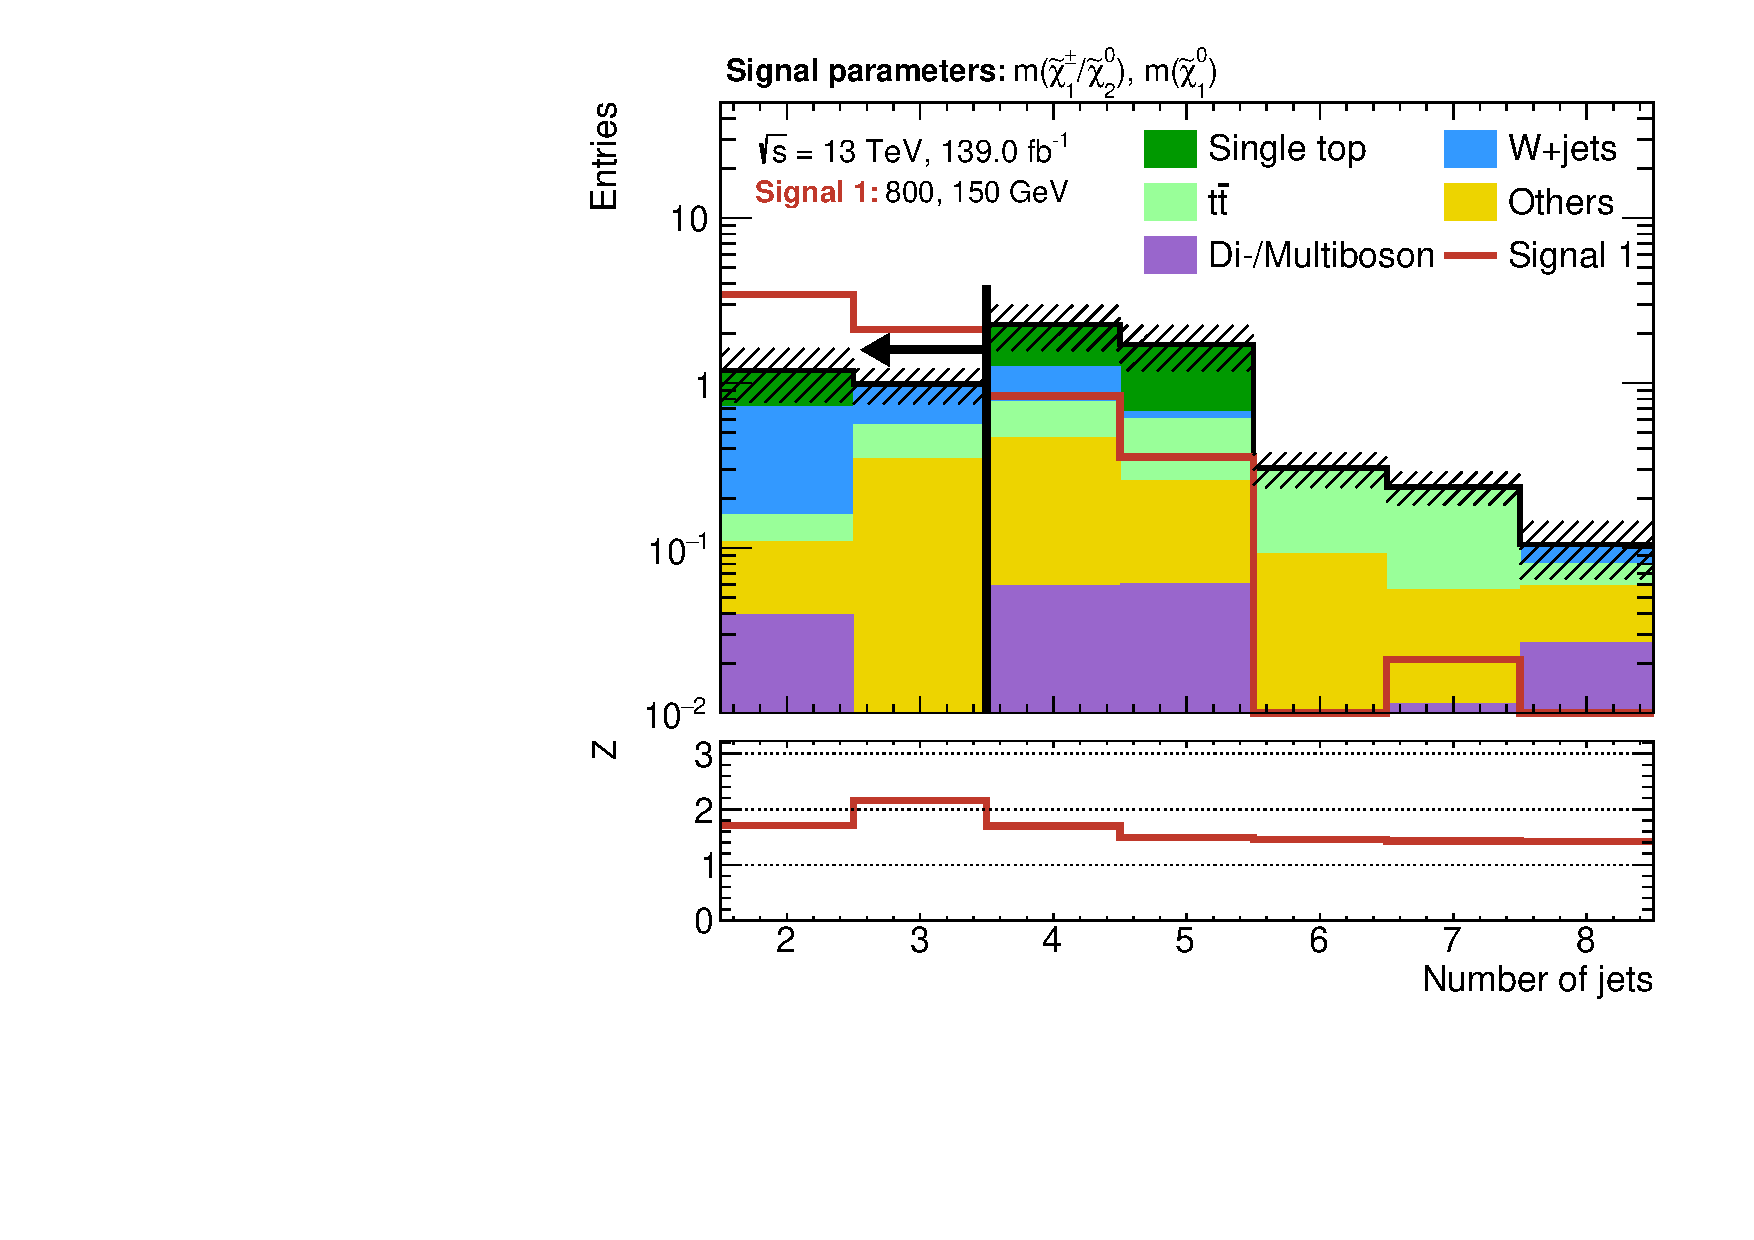
\includegraphics[width=0.9\textwidth]{N-1_cut_scan/n1_800_150/nJet30}
	\end{subfigure}

	\caption[N-1 plots for the chosen cut combination for the (800, 150) signal point]{N-1 plots for the chosen cut combination for the $(m(\charg/\neutr), m(\lsp)) = (\SI{800}{\GeV}, \SI{150}{\GeV})$ signal point. The shaded region includes \gls{mc} statistical as well as 30\% systematic uncertainties (added in quadrature) on the background. The significance is computed using the binomial discovery significance using the uncertainty on the background.}
	\label{fig:results_n1_800_150}
\end{figure}

\begin{figure}
	\centering
	\begin{subfigure}[b]{0.5\linewidth}
		\centering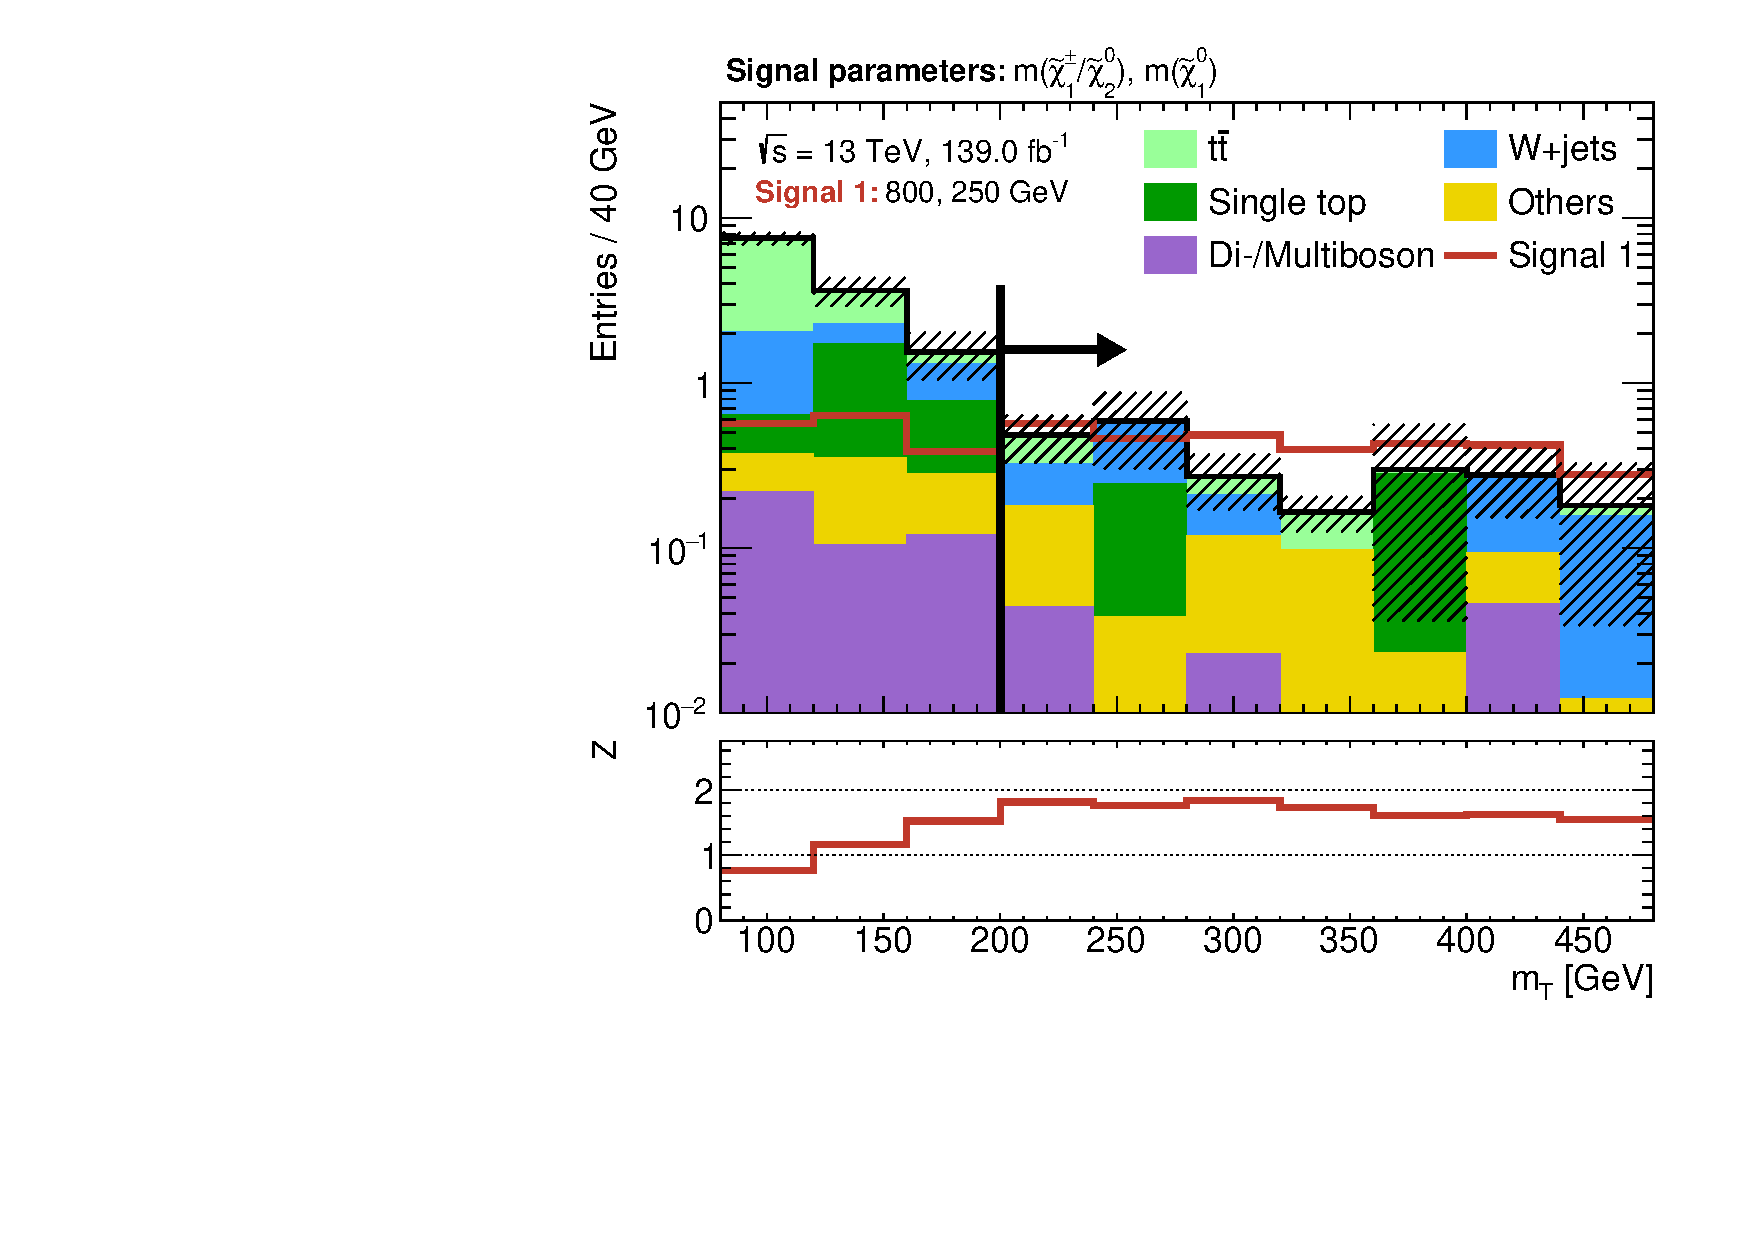
\includegraphics[width=0.9\textwidth]{N-1_cut_scan/n1_800_250/mt}
	\end{subfigure}\hfill
	\begin{subfigure}[b]{0.5\linewidth}
		\centering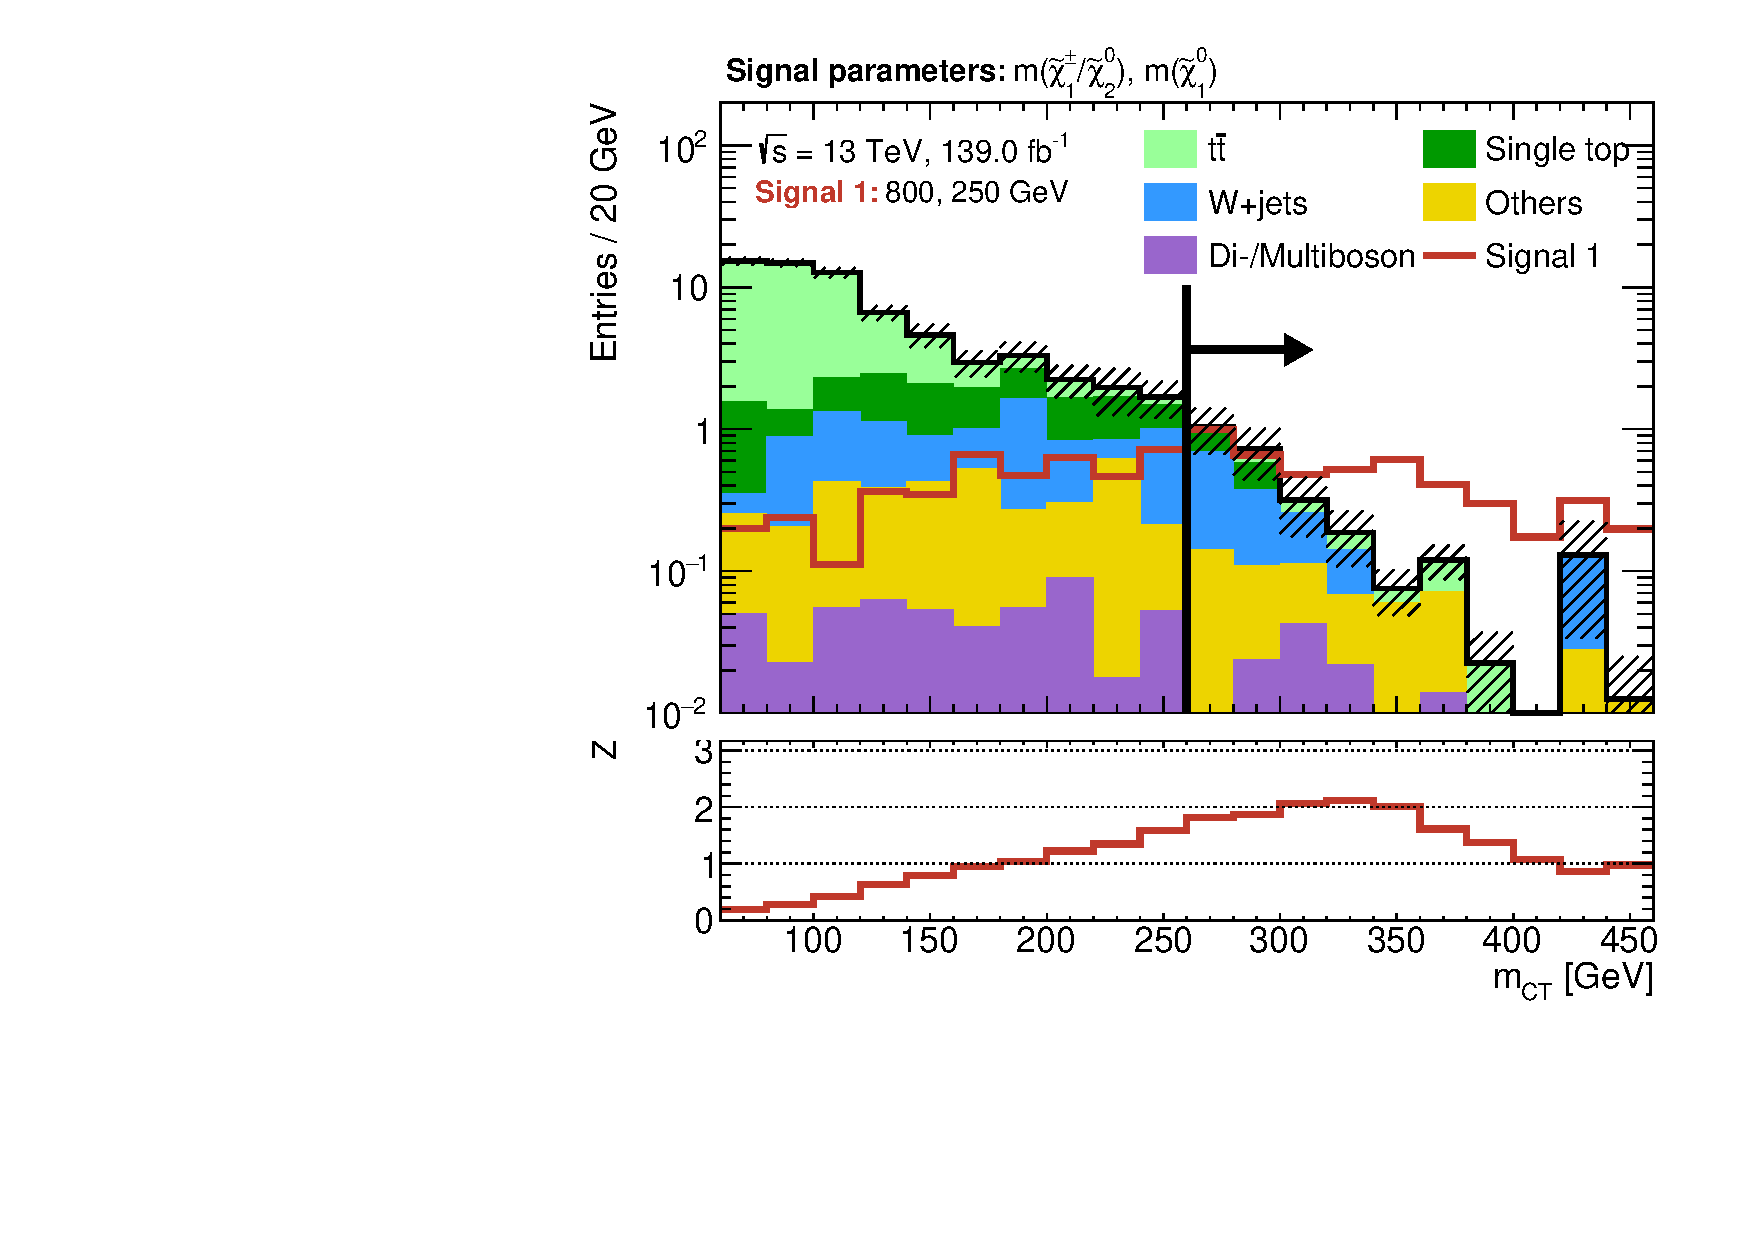
\includegraphics[width=0.9\textwidth]{N-1_cut_scan/n1_800_250/mct}
	\end{subfigure}\hfill
	\begin{subfigure}[b]{0.5\linewidth}
		\centering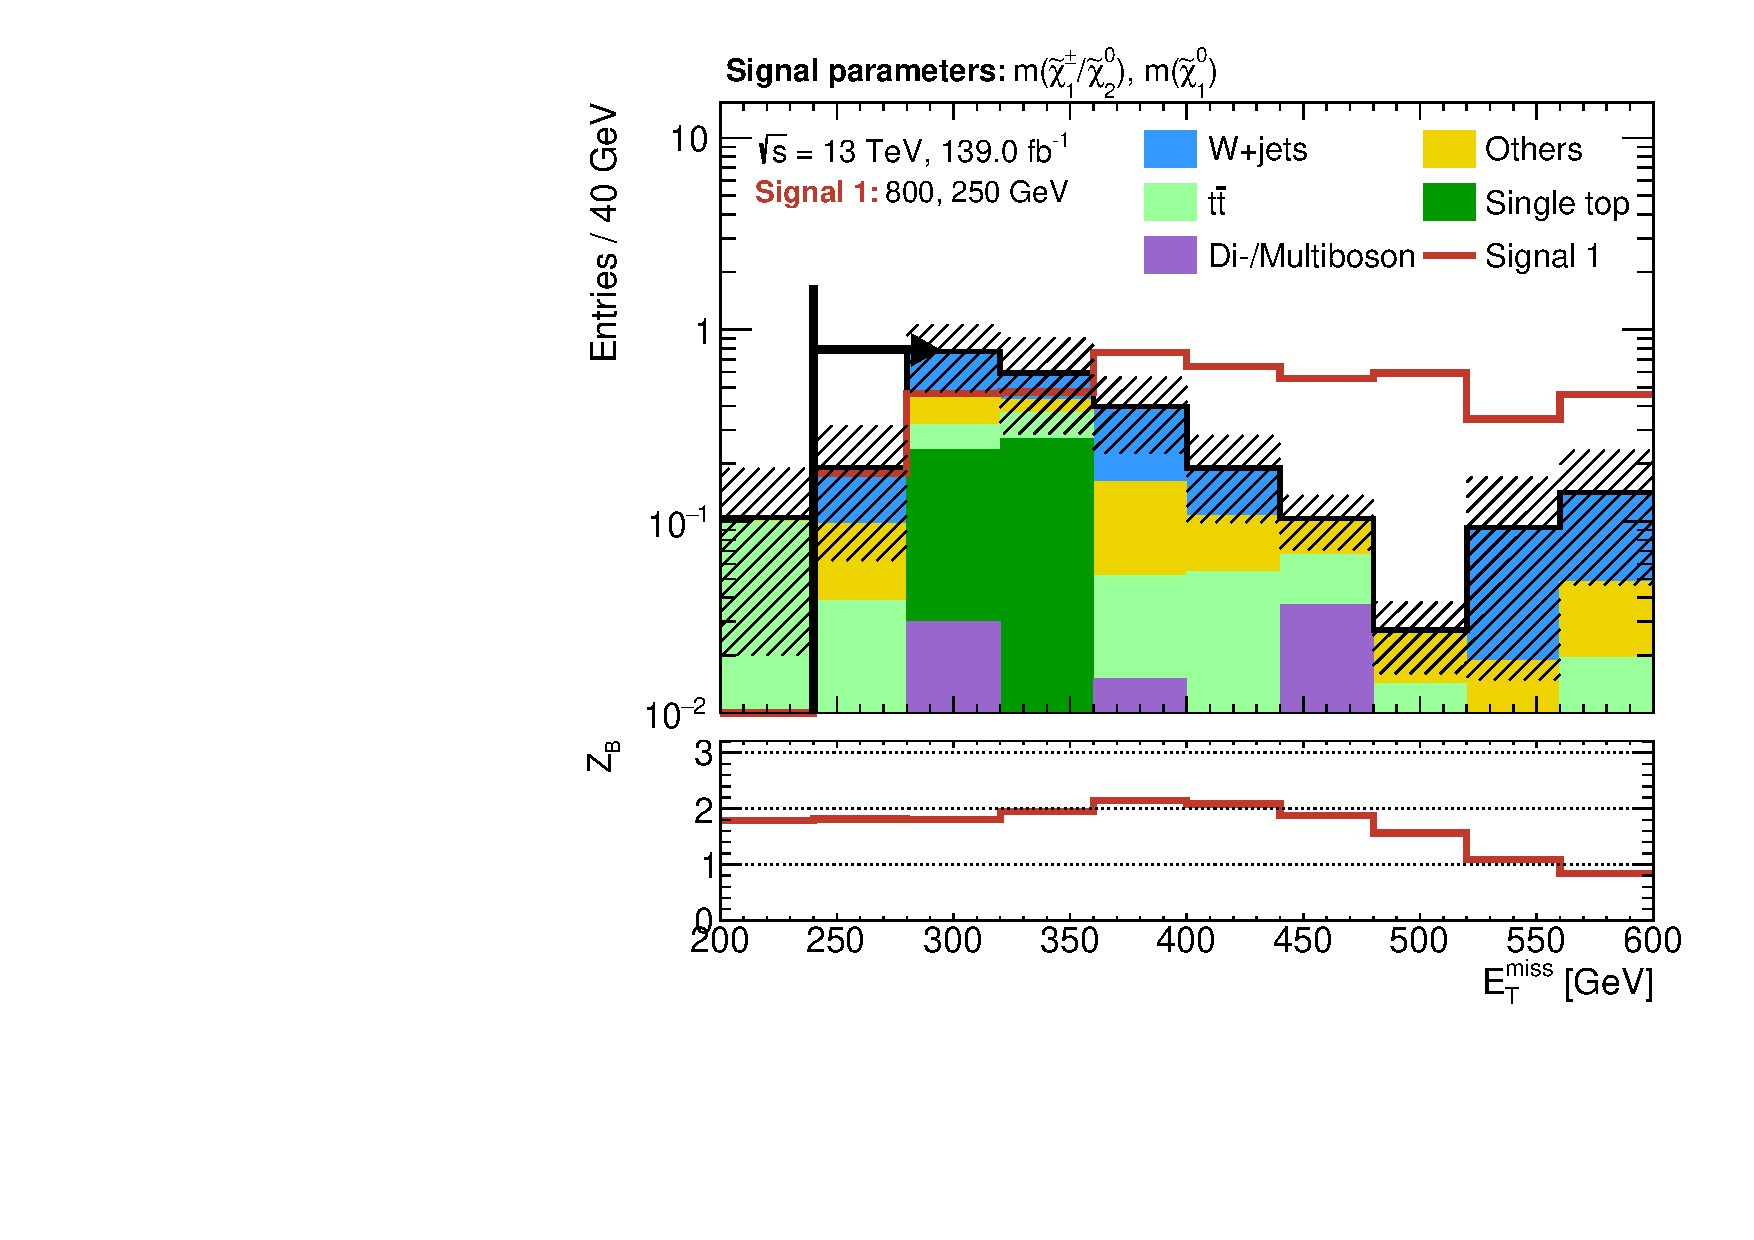
\includegraphics[width=0.9\textwidth]{N-1_cut_scan/n1_800_250/met}
	\end{subfigure}\hfill
	\begin{subfigure}[b]{0.5\linewidth}
		\centering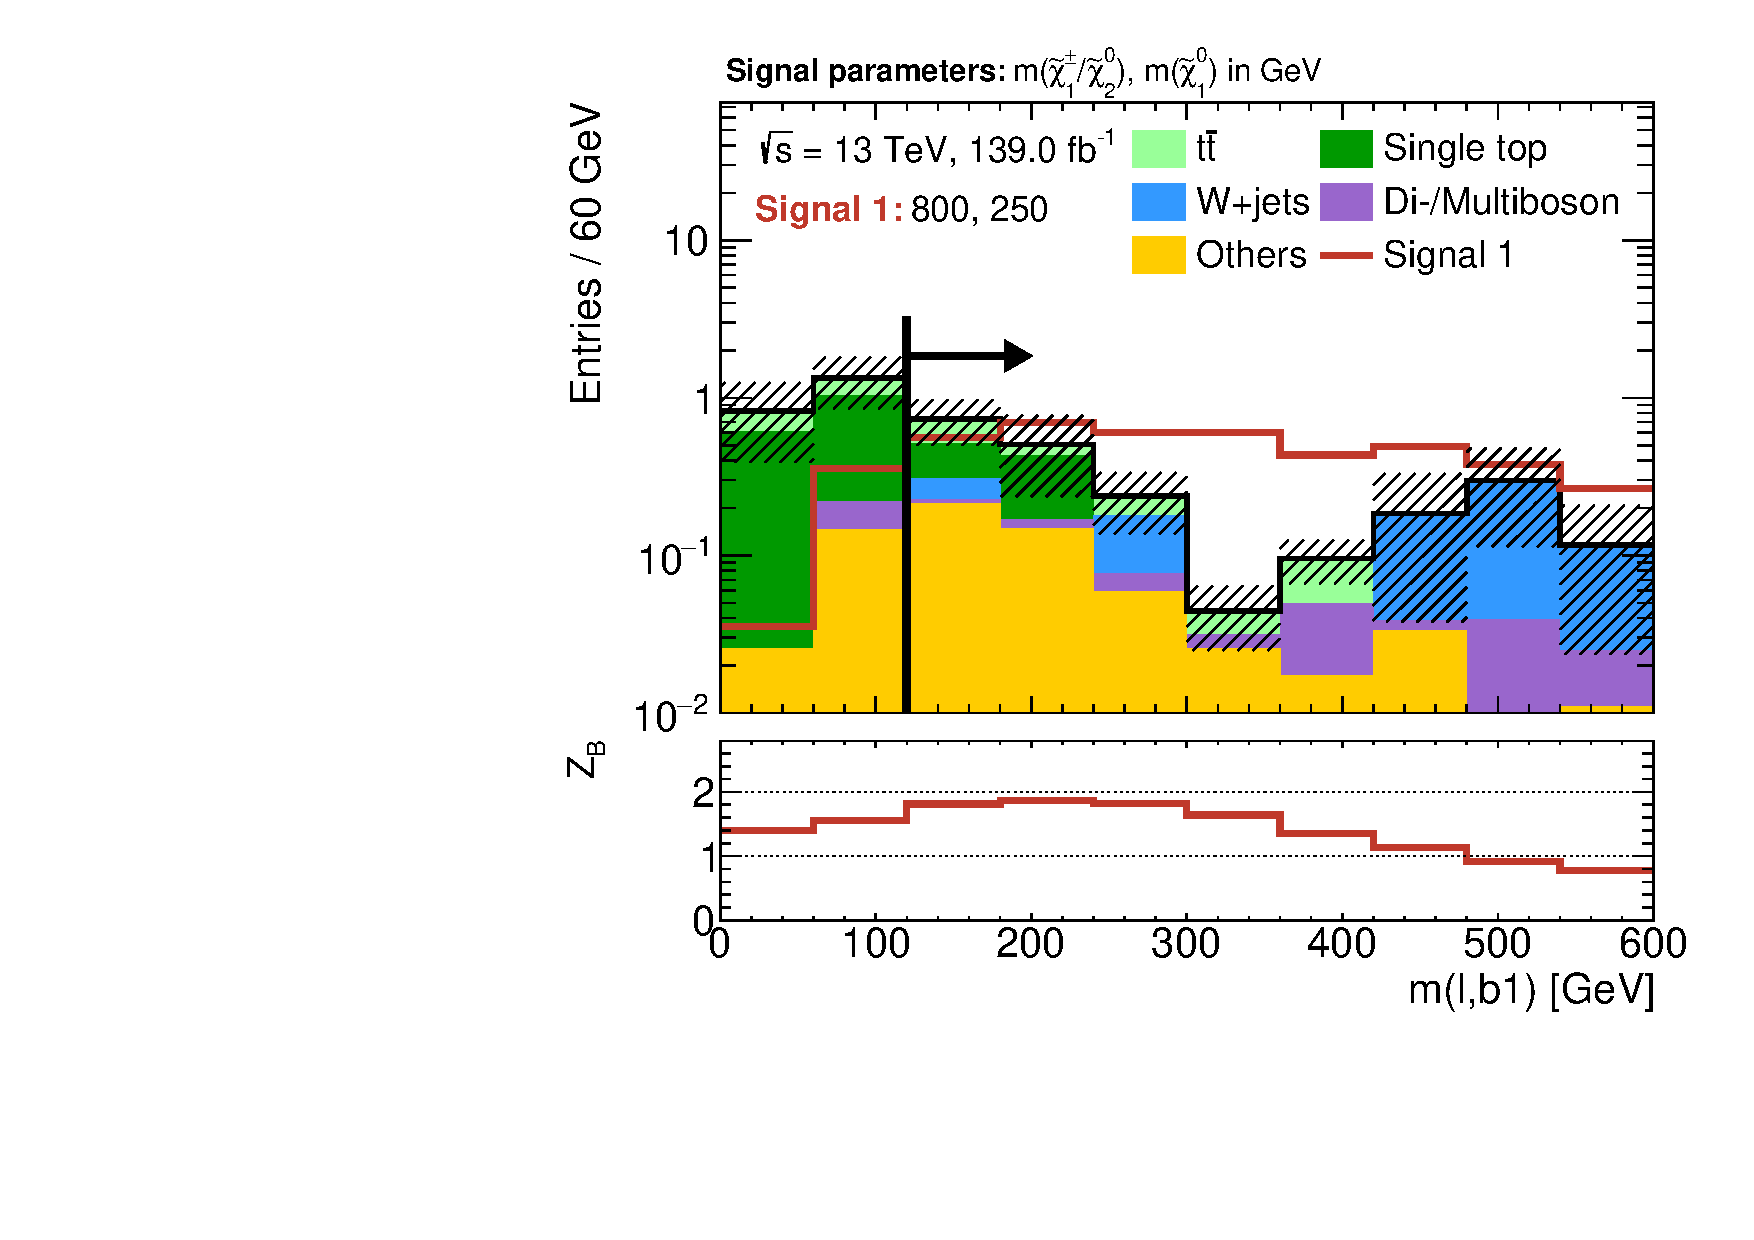
\includegraphics[width=0.9\textwidth]{N-1_cut_scan/n1_800_250/mlb1}
	\end{subfigure}\hfill
	\begin{subfigure}[b]{0.5\linewidth}
		\centering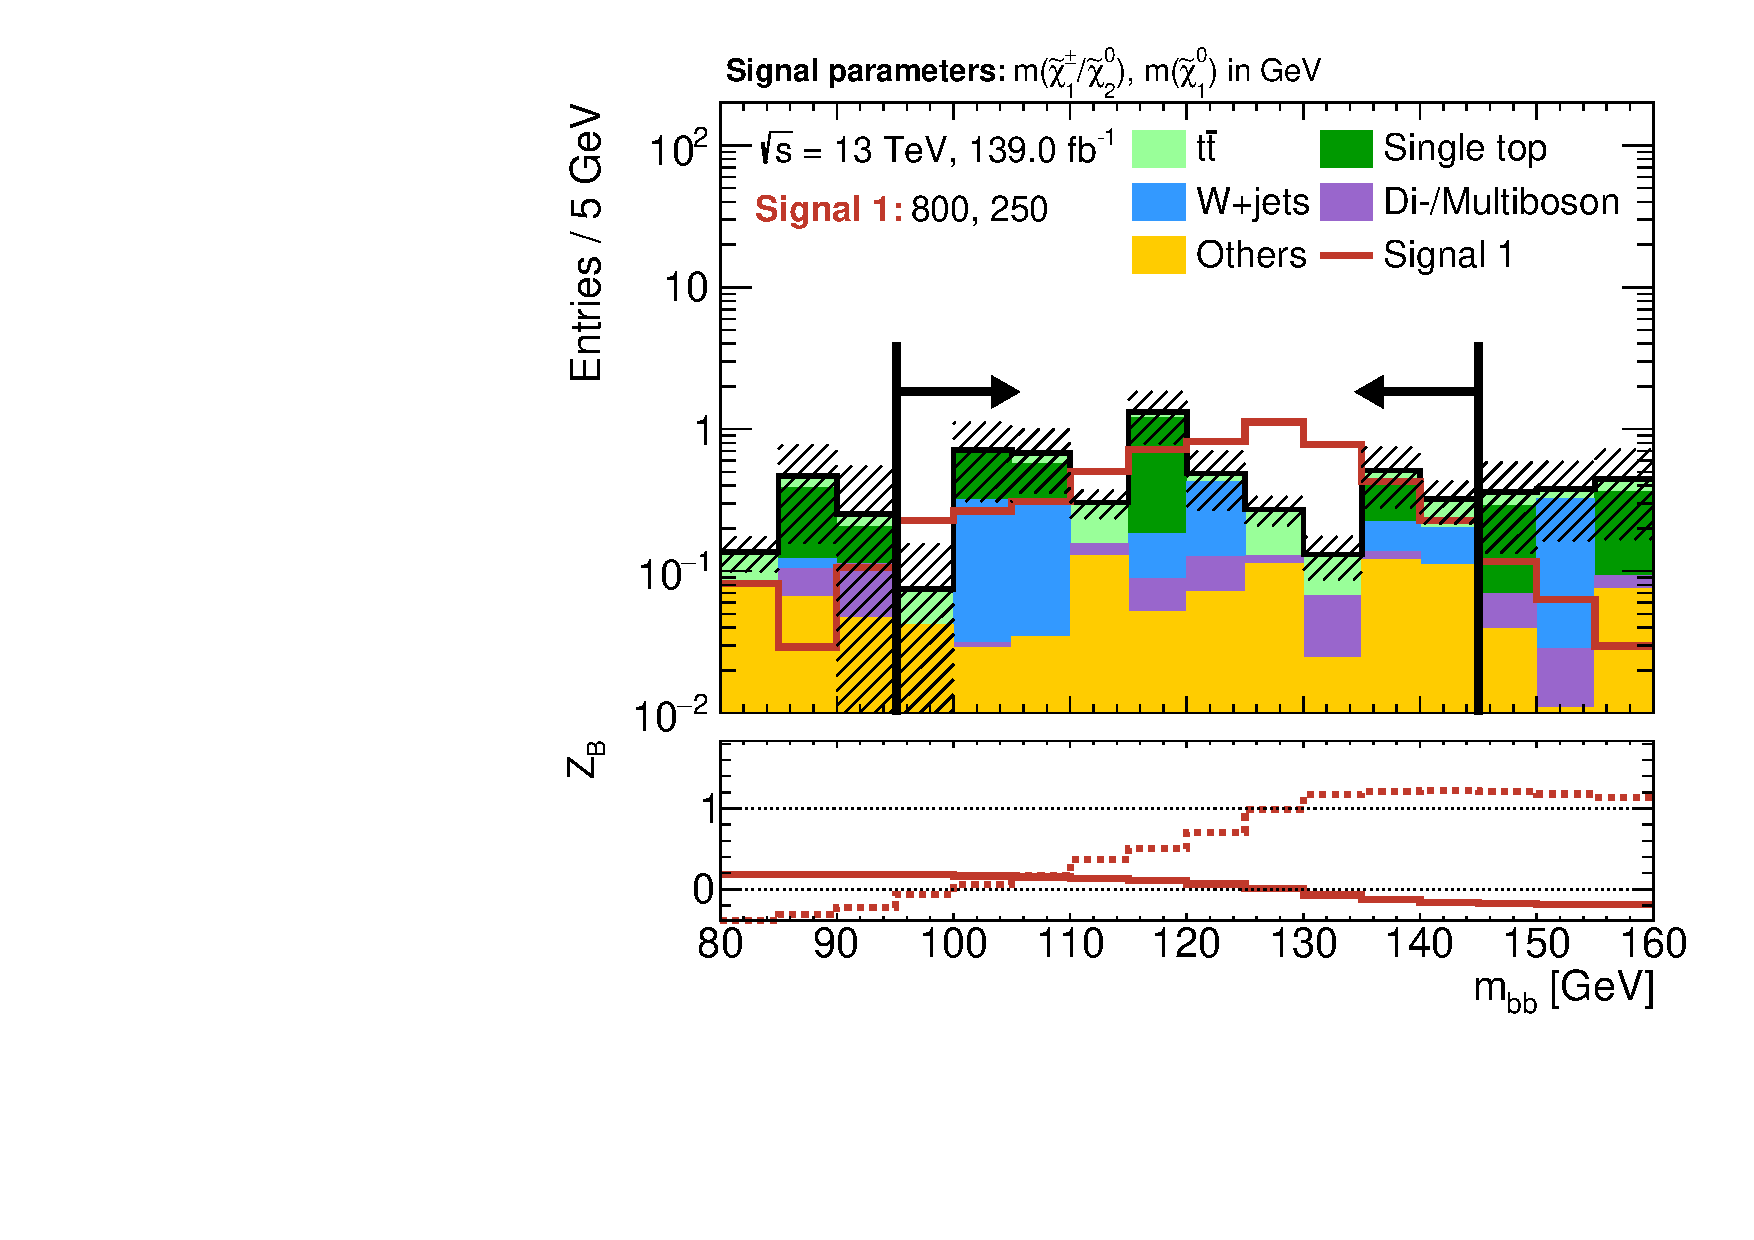
\includegraphics[width=0.9\textwidth]{N-1_cut_scan/n1_800_250/mbb_both}
	\end{subfigure}\hfill
	\begin{subfigure}[b]{0.5\linewidth}
		\centering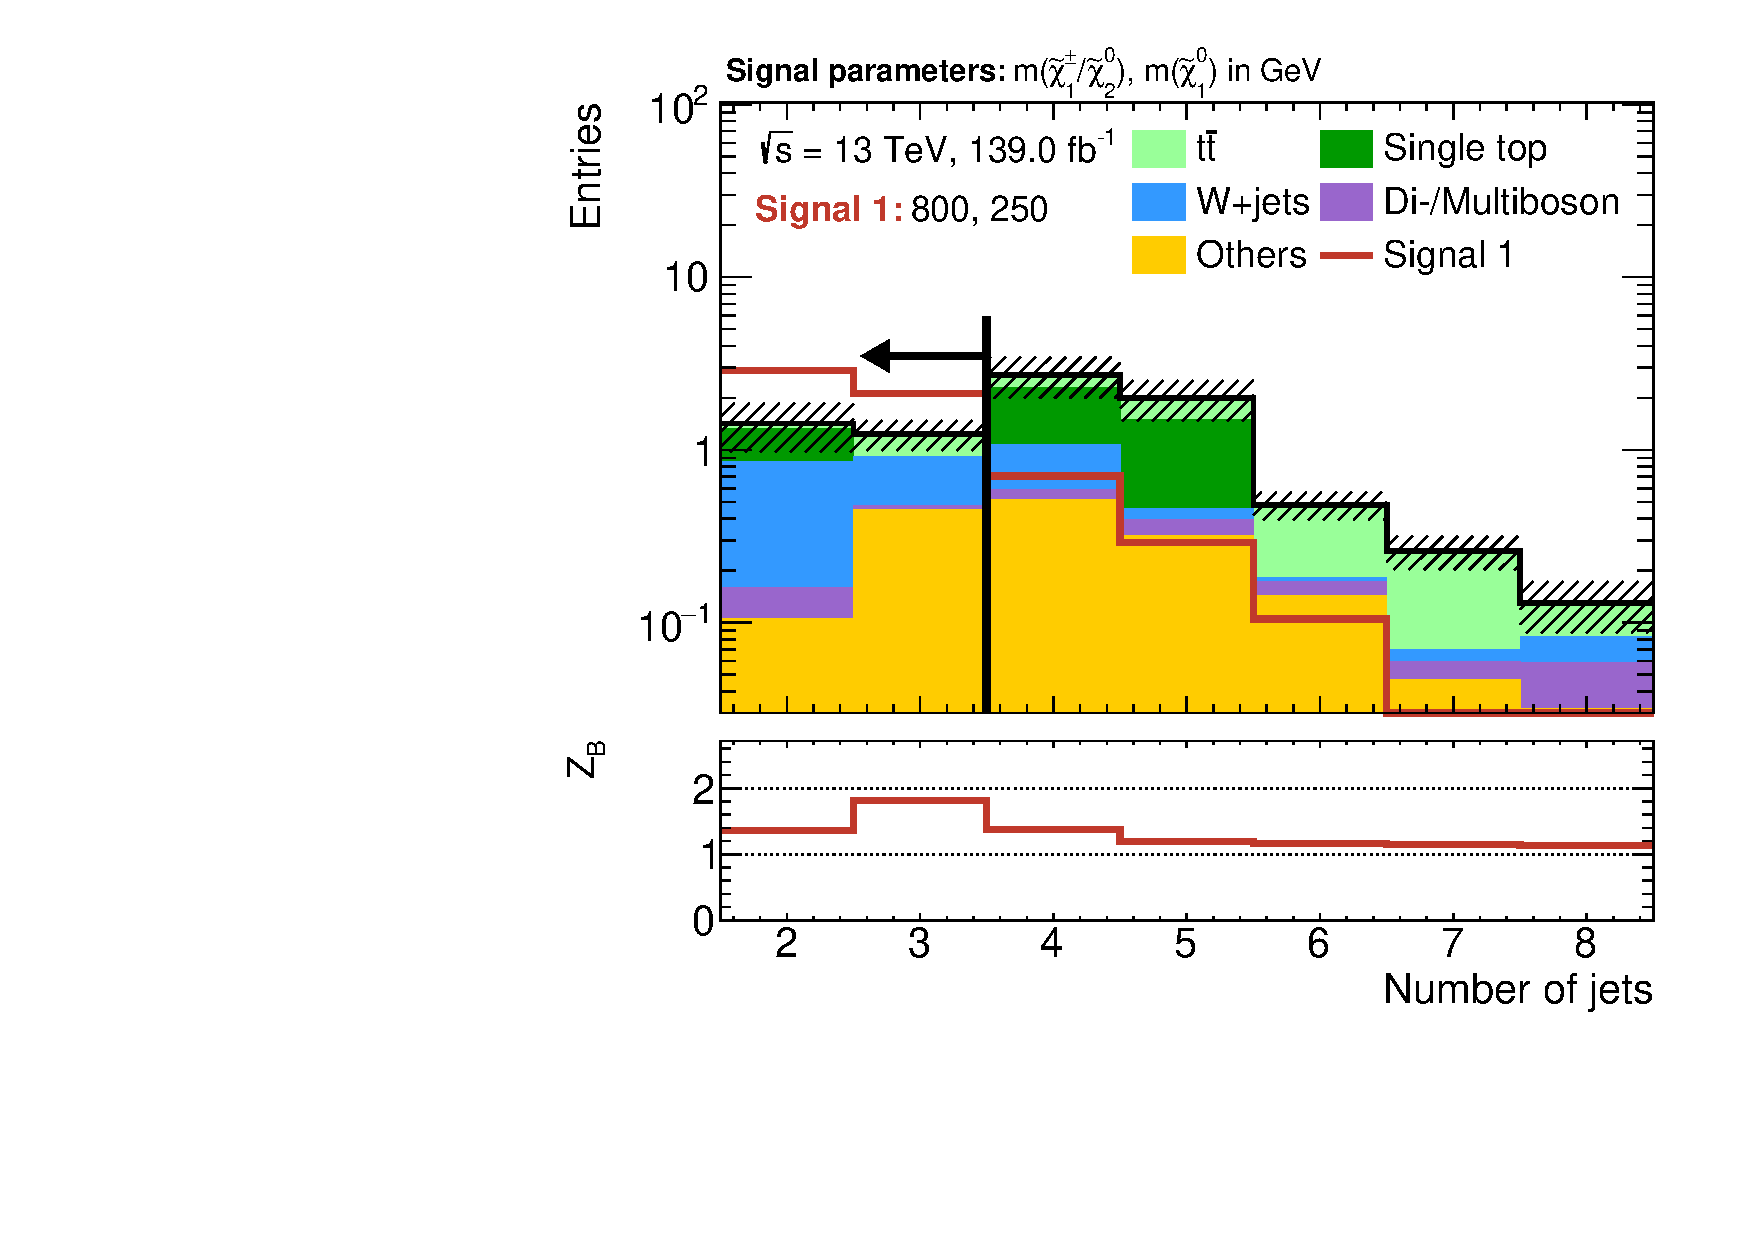
\includegraphics[width=0.9\textwidth]{N-1_cut_scan/n1_800_250/nJet30}
	\end{subfigure}

	\caption[\textit{N}--1 plots for the chosen cut combination for the (800, 250) signal point]{\textit{N}--1 plots for the chosen cut combination for the $(m(\charg/\neutr), m(\lsp)) = (\SI{800}{\GeV}, \SI{250}{\GeV})$ signal point. The shaded region includes \gls{mc} statistical as well as 30\% systematic uncertainties (added in quadrature) on the background. The significance is computed using the binomial discovery significance using the uncertainty on the background.}
	\label{fig:results_n1_800_250}
\end{figure}

\begin{figure}
	\centering
	\begin{subfigure}[b]{0.5\linewidth}
		\centering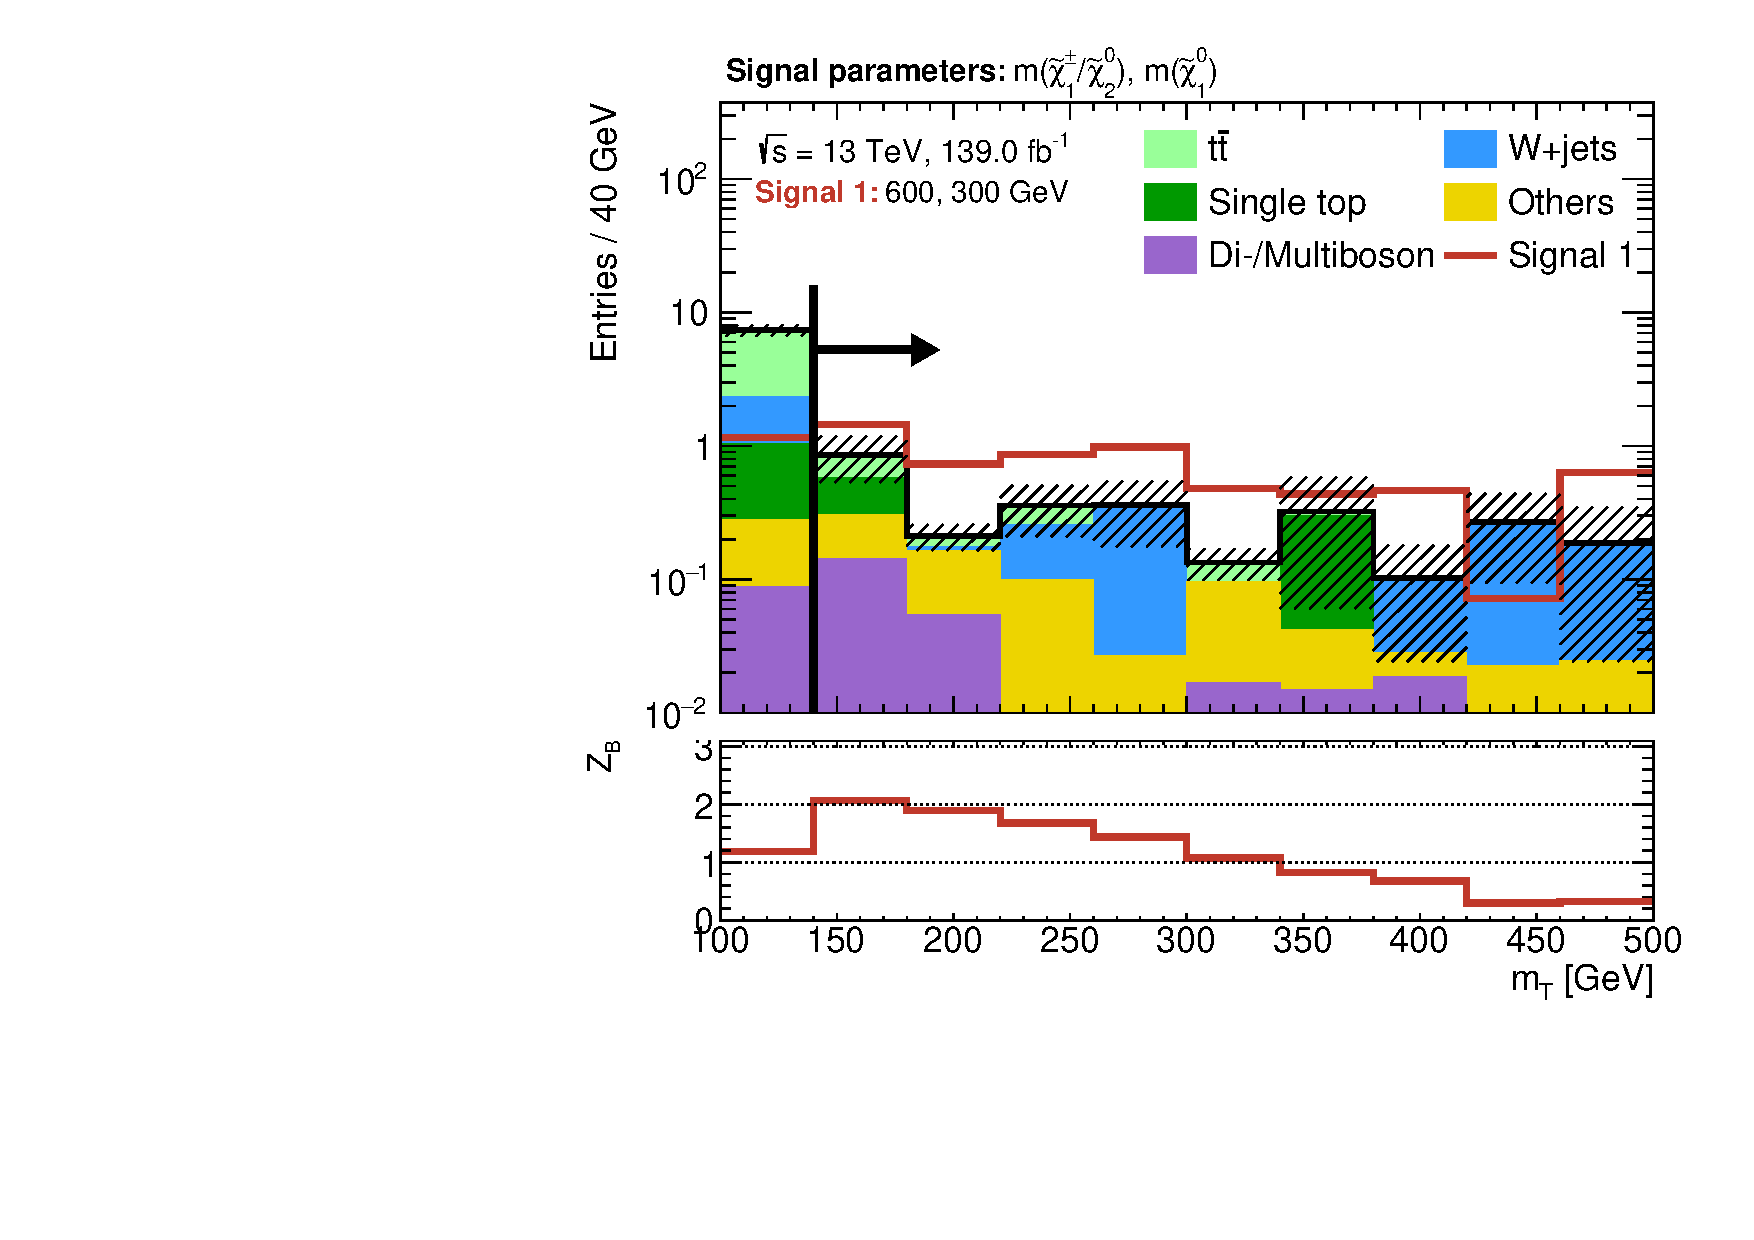
\includegraphics[width=0.9\textwidth]{N-1_cut_scan/n1_600_300/mt}
	\end{subfigure}\hfill
	\begin{subfigure}[b]{0.5\linewidth}
		\centering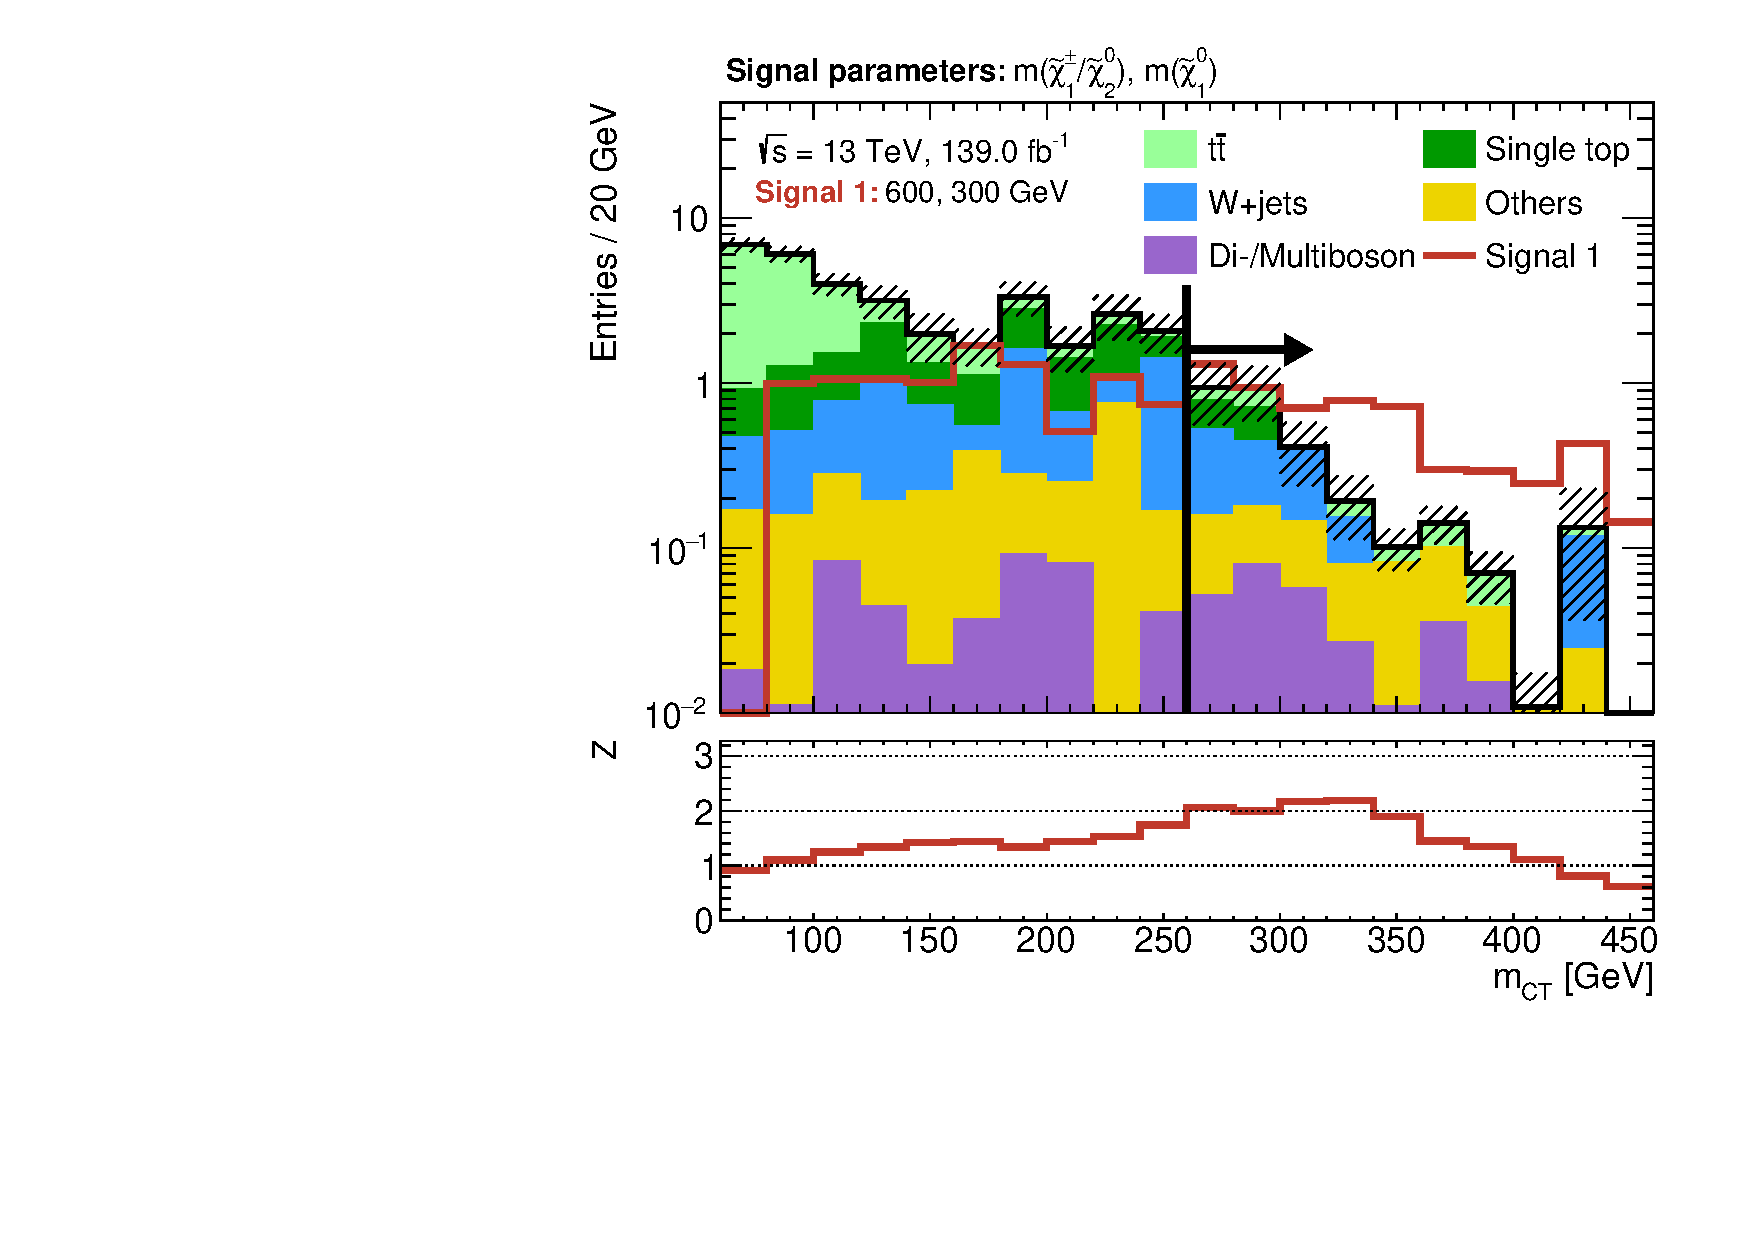
\includegraphics[width=0.9\textwidth]{N-1_cut_scan/n1_600_300/mct}
	\end{subfigure}\hfill
	\begin{subfigure}[b]{0.5\linewidth}
		\centering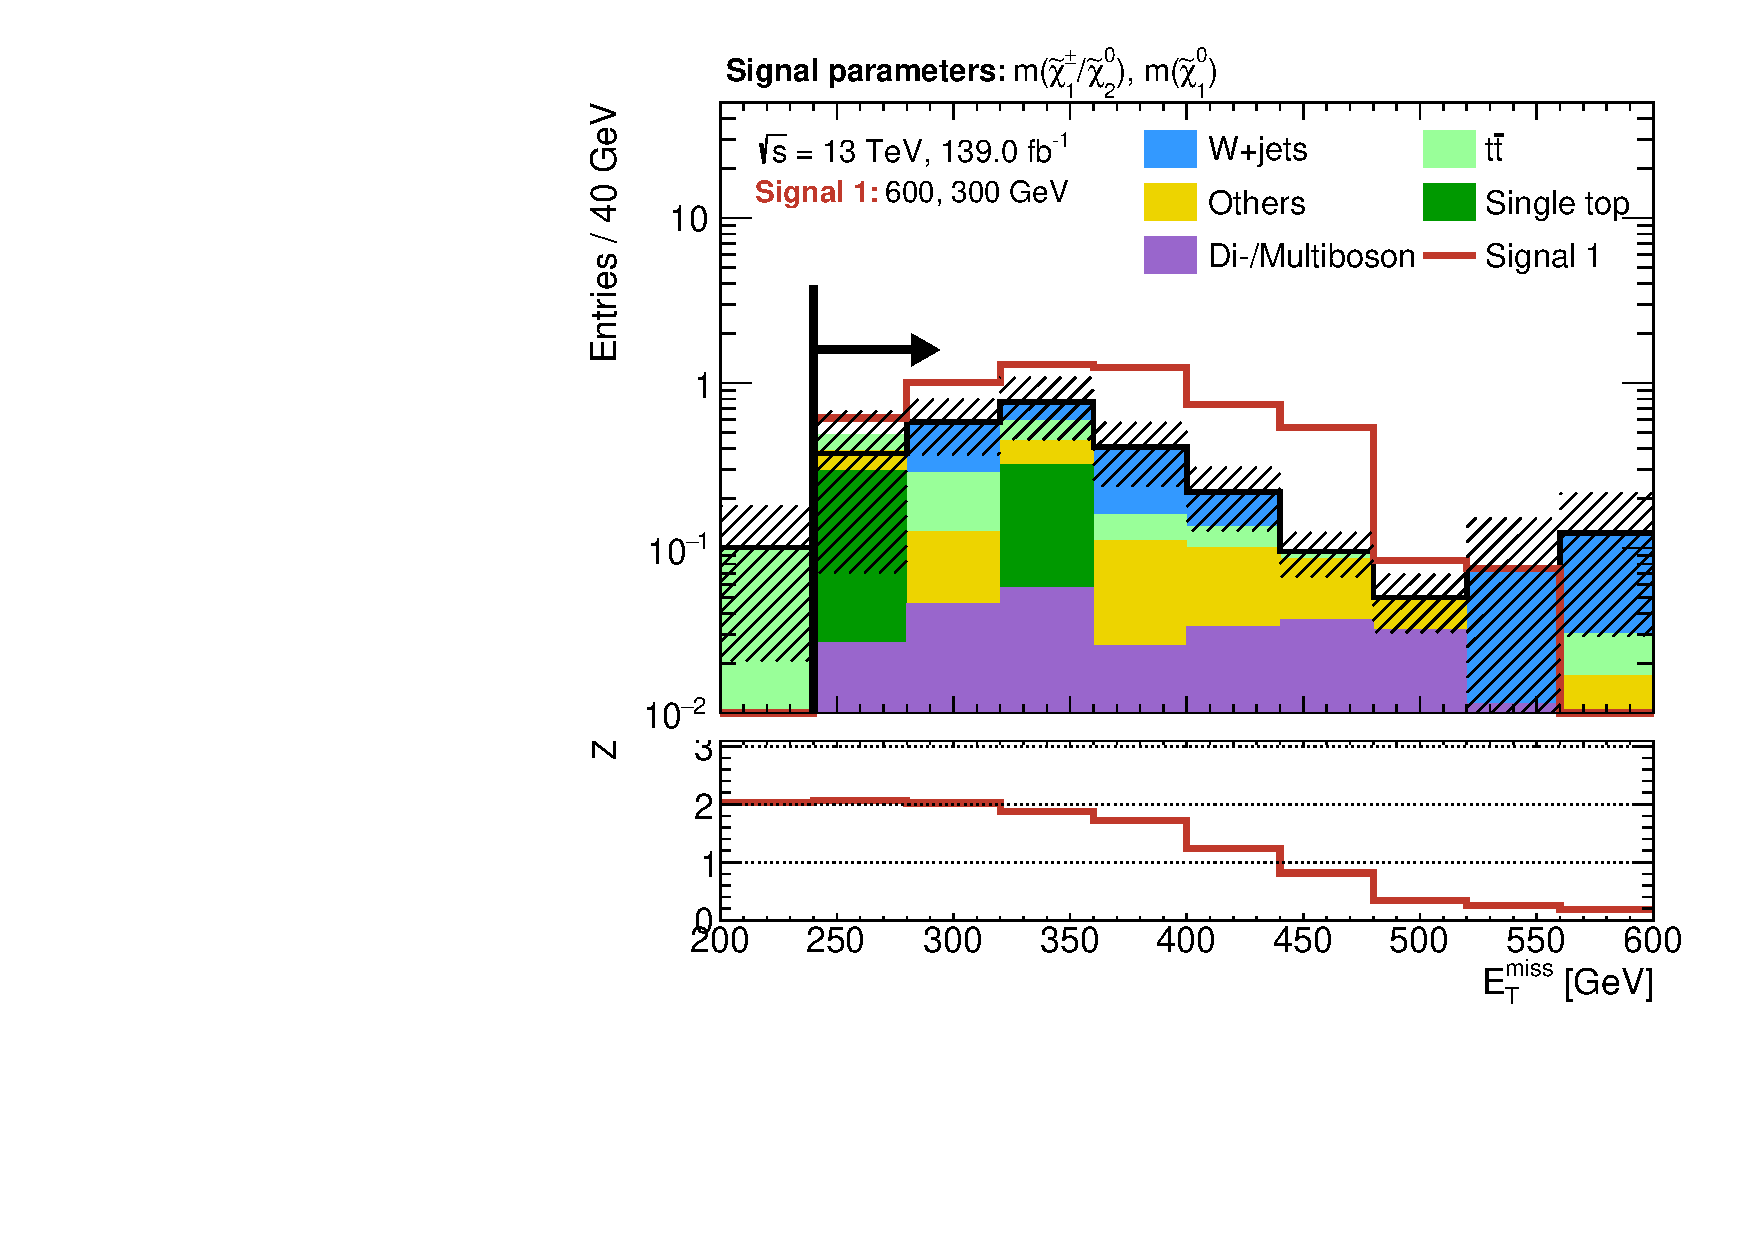
\includegraphics[width=0.9\textwidth]{N-1_cut_scan/n1_600_300/met}
	\end{subfigure}\hfill
	\begin{subfigure}[b]{0.5\linewidth}
		\centering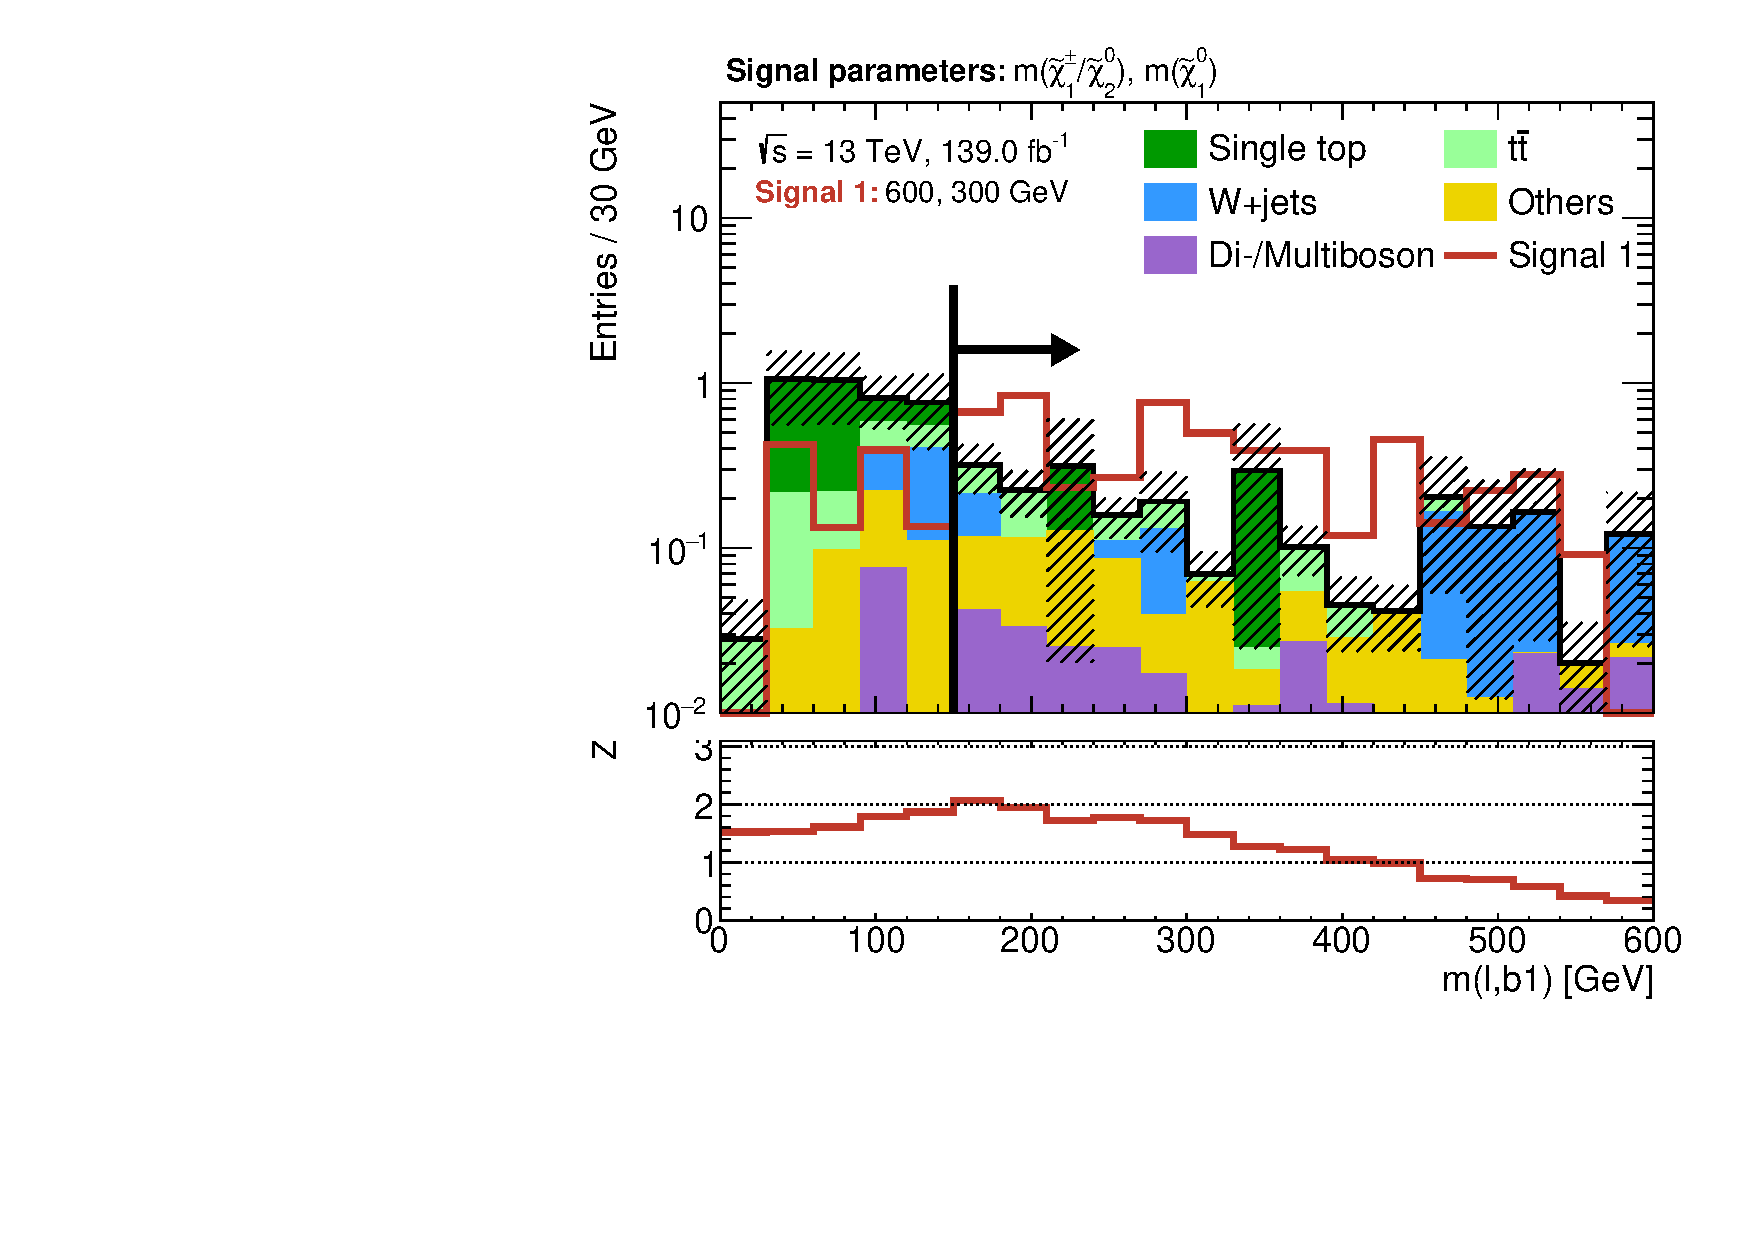
\includegraphics[width=0.9\textwidth]{N-1_cut_scan/n1_600_300/mlb1}
	\end{subfigure}\hfill
	\begin{subfigure}[b]{0.5\linewidth}
		\centering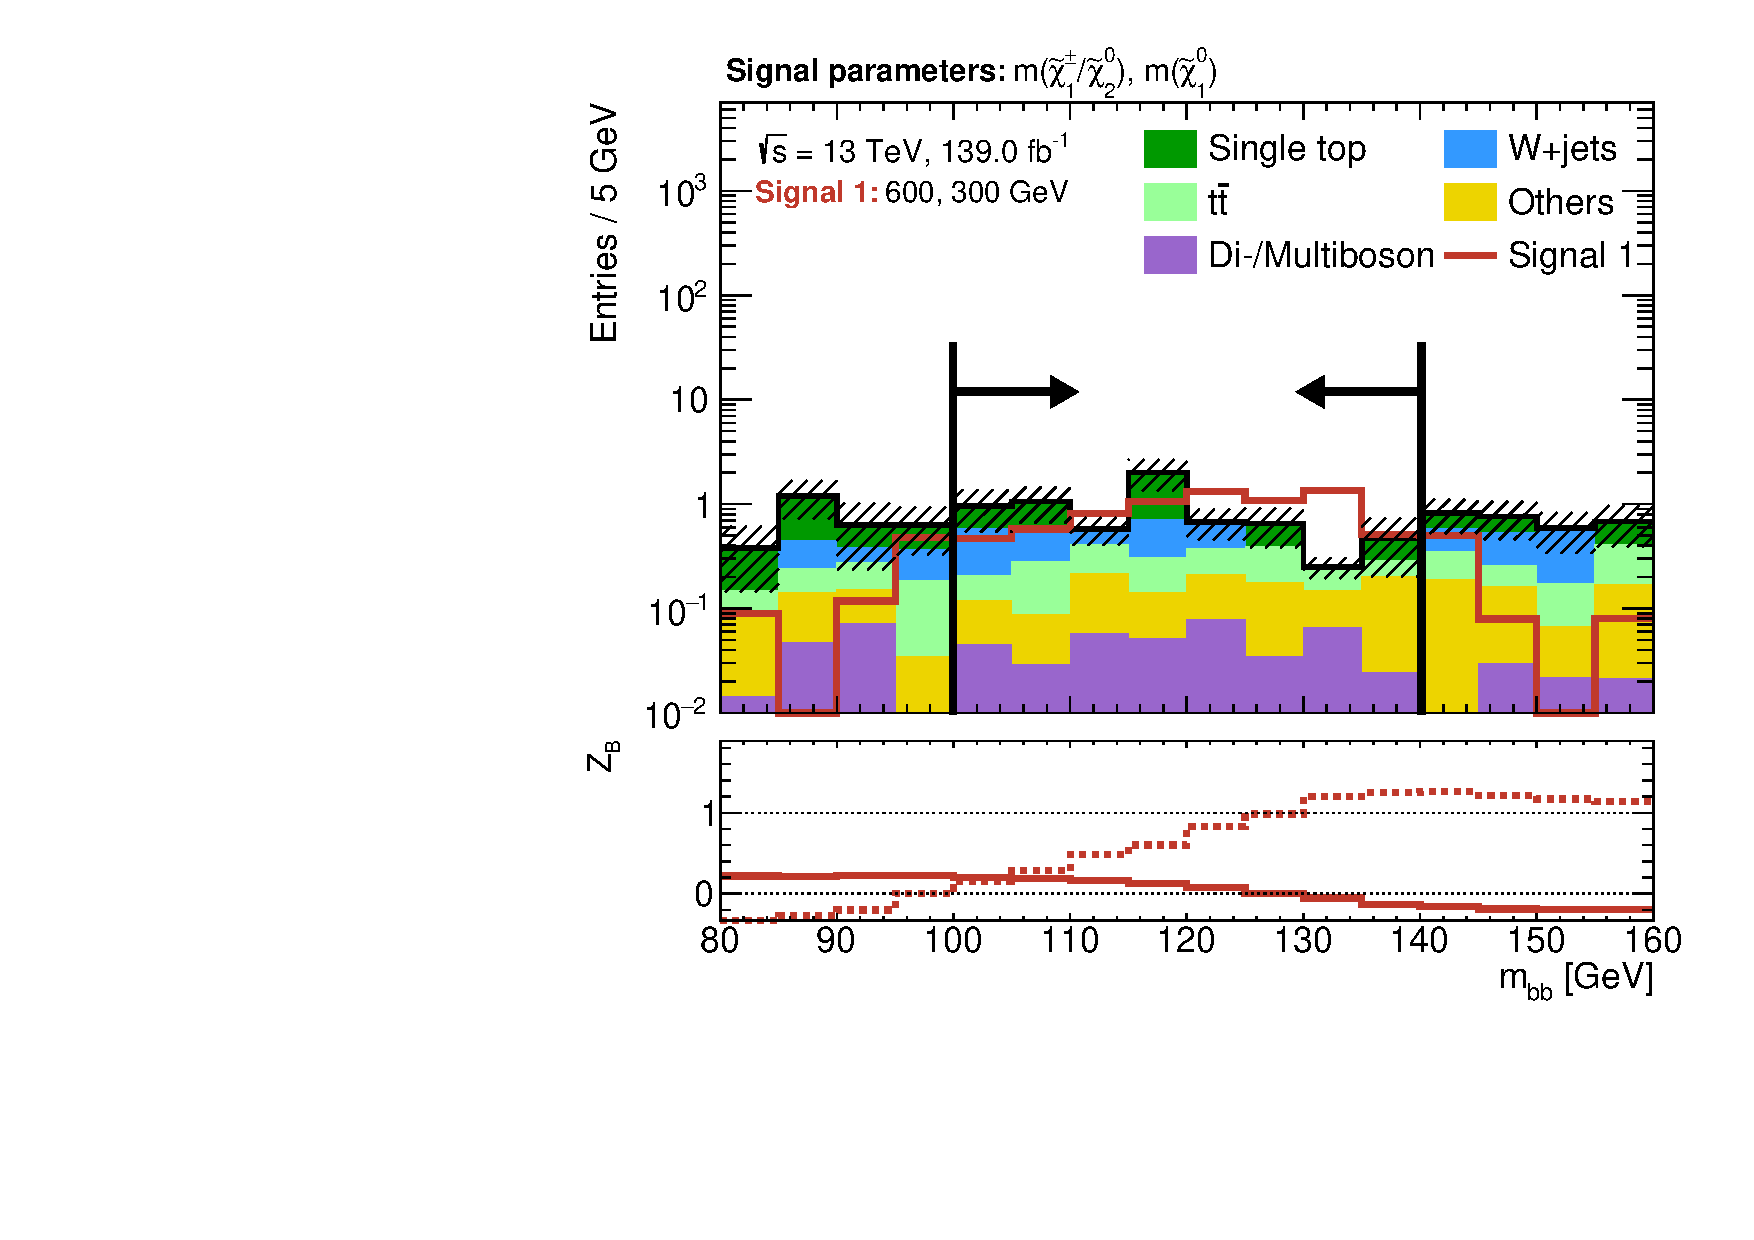
\includegraphics[width=0.9\textwidth]{N-1_cut_scan/n1_600_300/mbb_both}
	\end{subfigure}\hfill
	\begin{subfigure}[b]{0.5\linewidth}
		\centering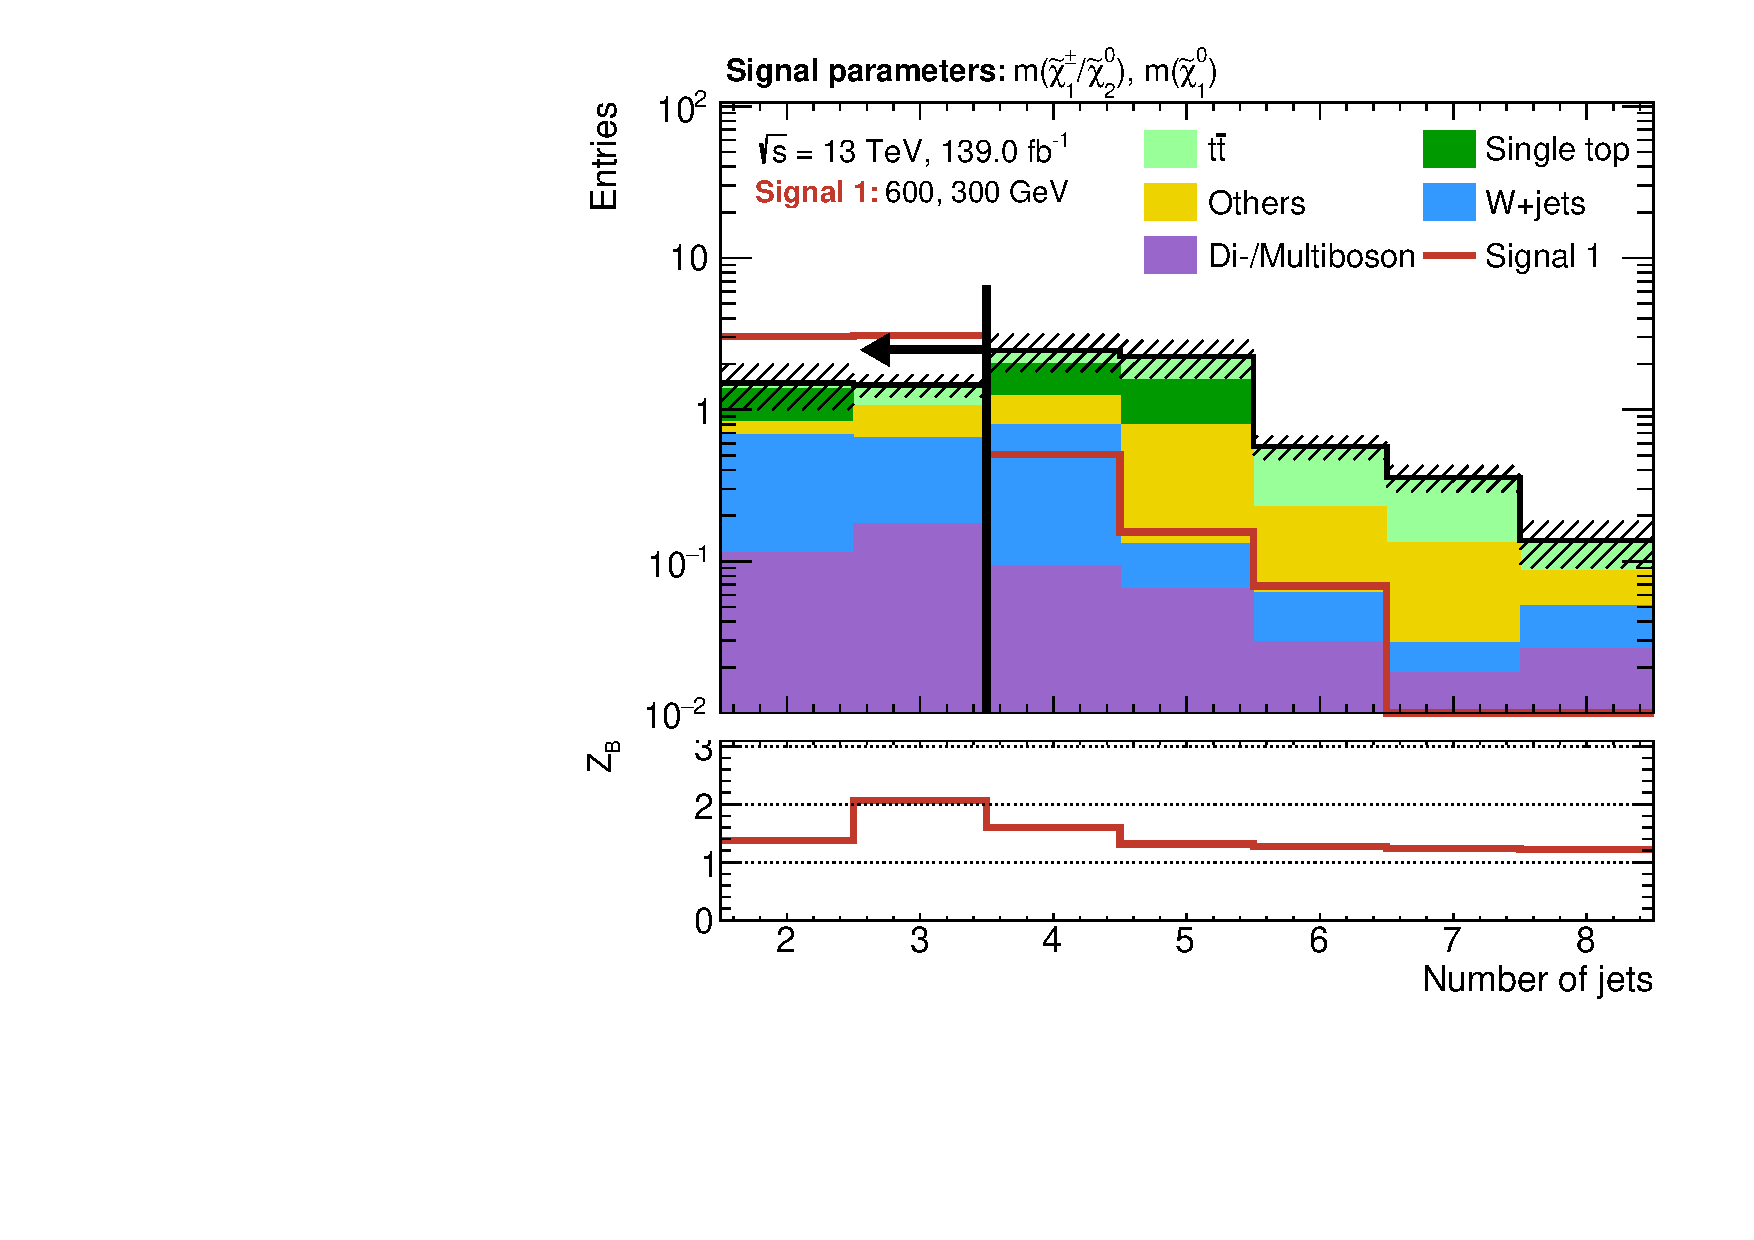
\includegraphics[width=0.9\textwidth]{N-1_cut_scan/n1_600_300/nJet30}
	\end{subfigure}

	\caption[\textit{N}--1 plots for the chosen cut combination for the (600, 300) signal point]{\textit{N}--1 plots for the chosen cut combination for the $(m(\charg/\neutr), m(\lsp)) = (\SI{600}{\GeV}, \SI{300}{\GeV})$ signal point. The shaded region includes \gls{mc} statistical as well as 30\% systematic uncertainties (added in quadrature) on the background. The significance is computed using the binomial discovery significance using the uncertainty on the background.}
	\label{fig:results_n1_600_300}
\end{figure}

\begin{figure}
	\centering
	\begin{subfigure}[b]{0.5\linewidth}
		\centering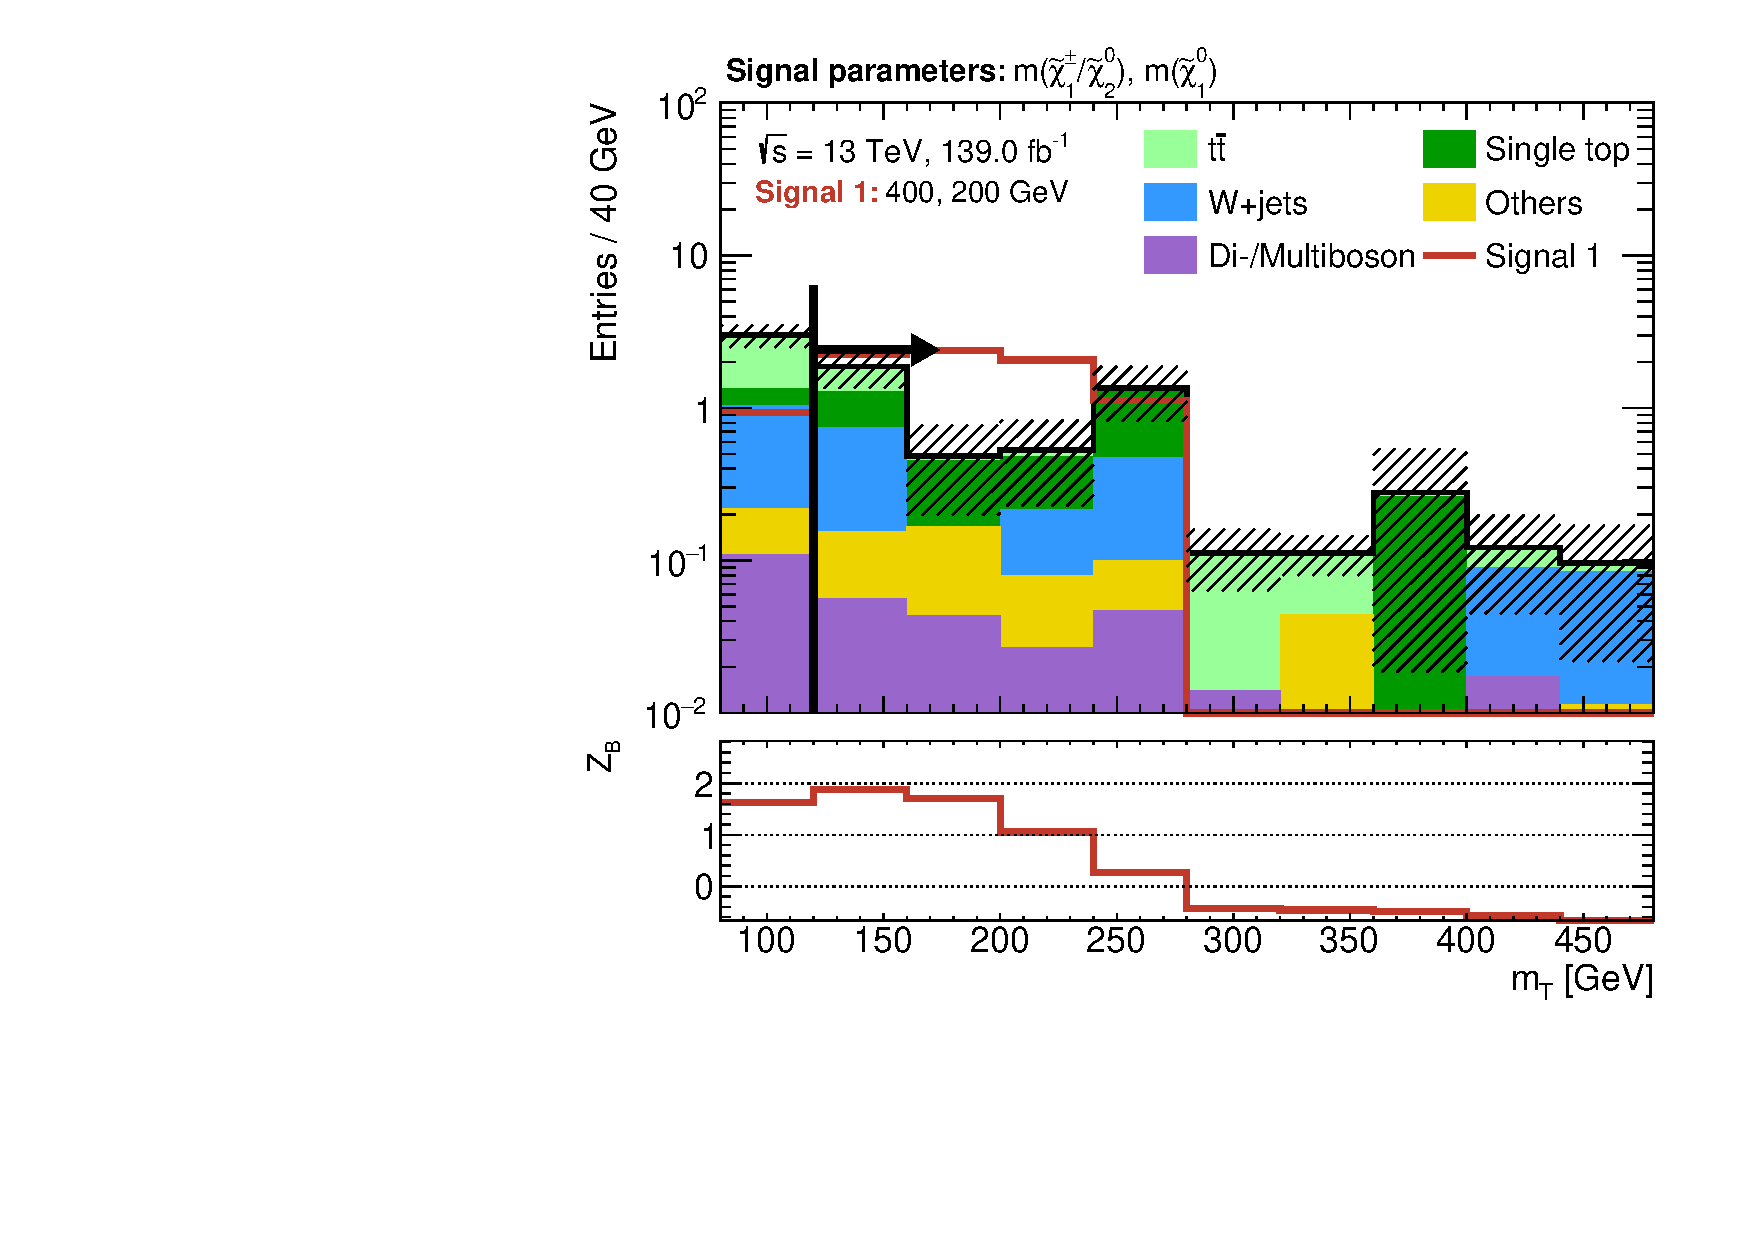
\includegraphics[width=0.9\textwidth]{N-1_cut_scan/n1_400_200/mt}
	\end{subfigure}\hfill
	\begin{subfigure}[b]{0.5\linewidth}
		\centering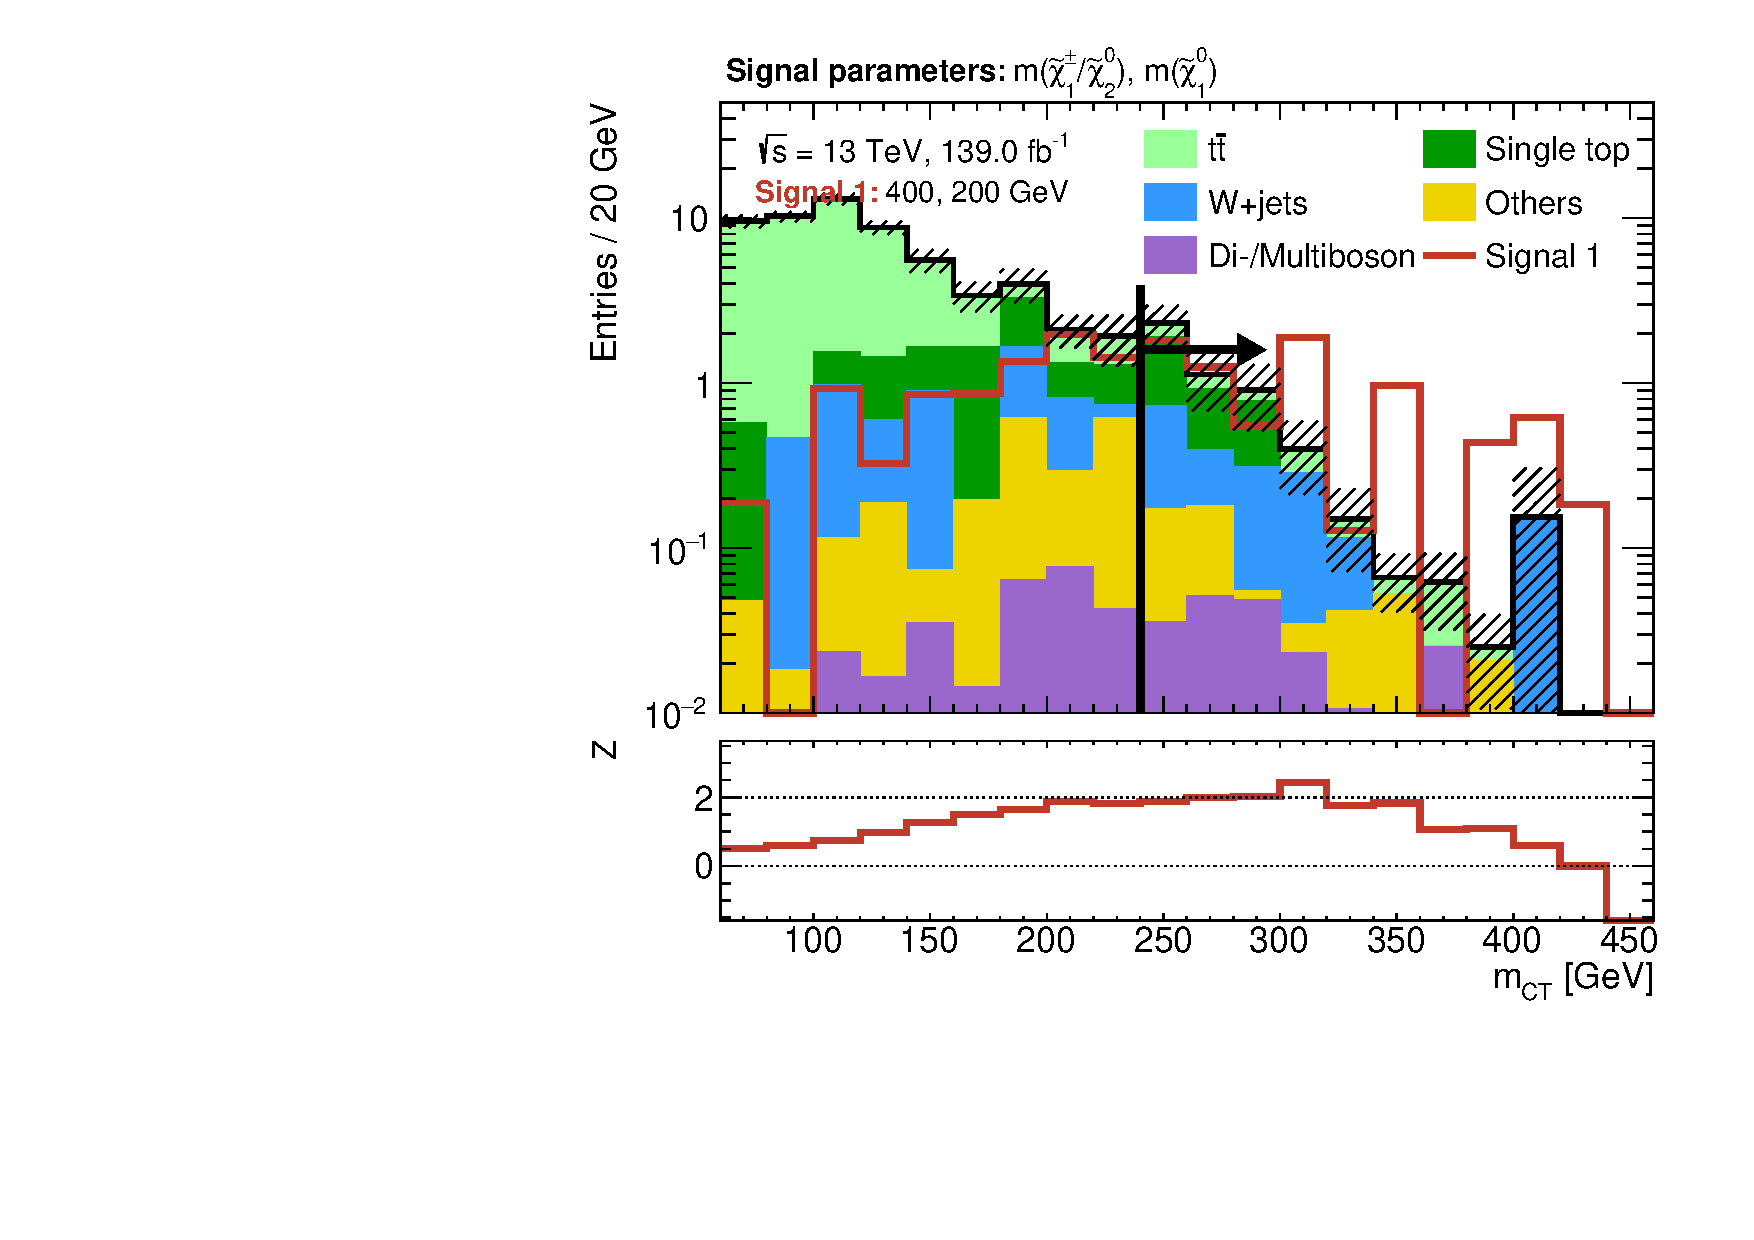
\includegraphics[width=0.9\textwidth]{N-1_cut_scan/n1_400_200/mct}
	\end{subfigure}\hfill
	\begin{subfigure}[b]{0.5\linewidth}
		\centering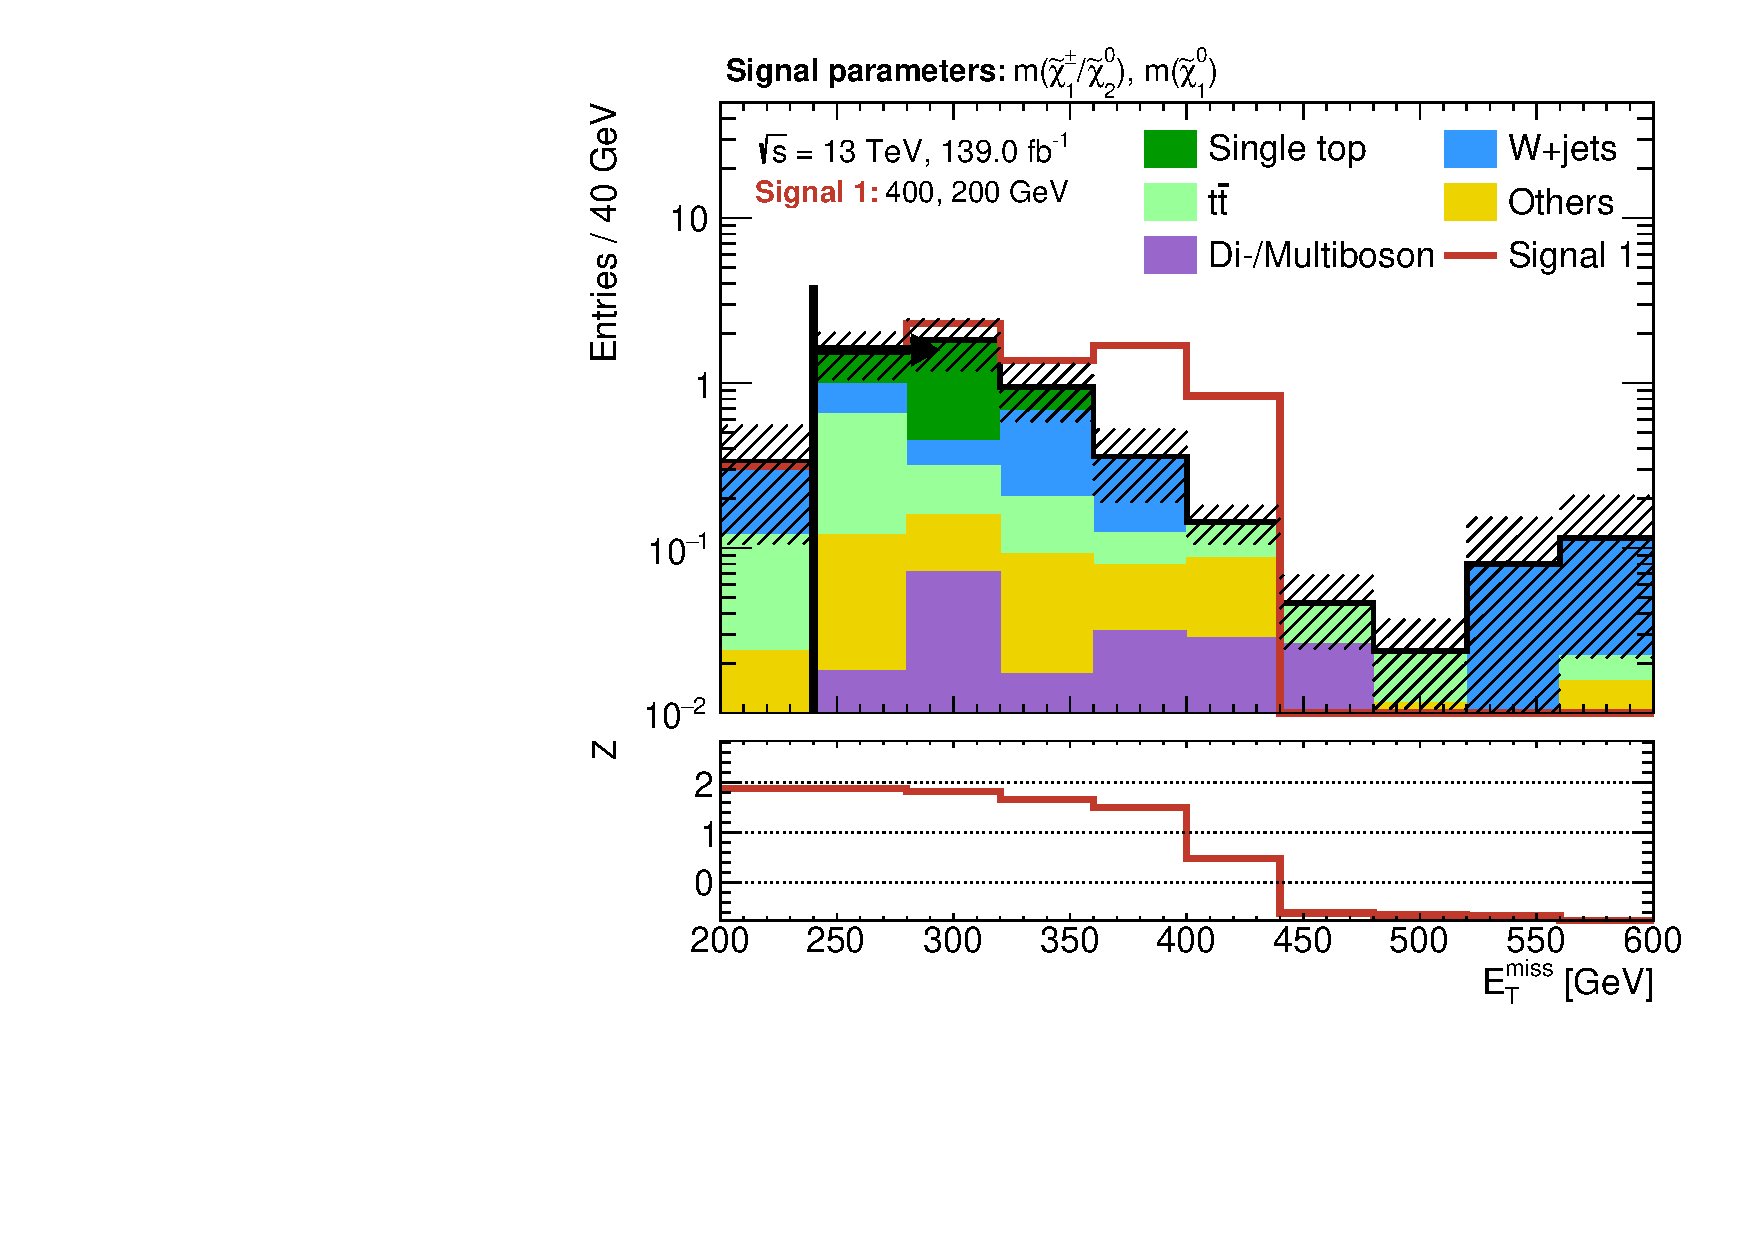
\includegraphics[width=0.9\textwidth]{N-1_cut_scan/n1_400_200/met}
	\end{subfigure}\hfill
	\begin{subfigure}[b]{0.5\linewidth}
		\centering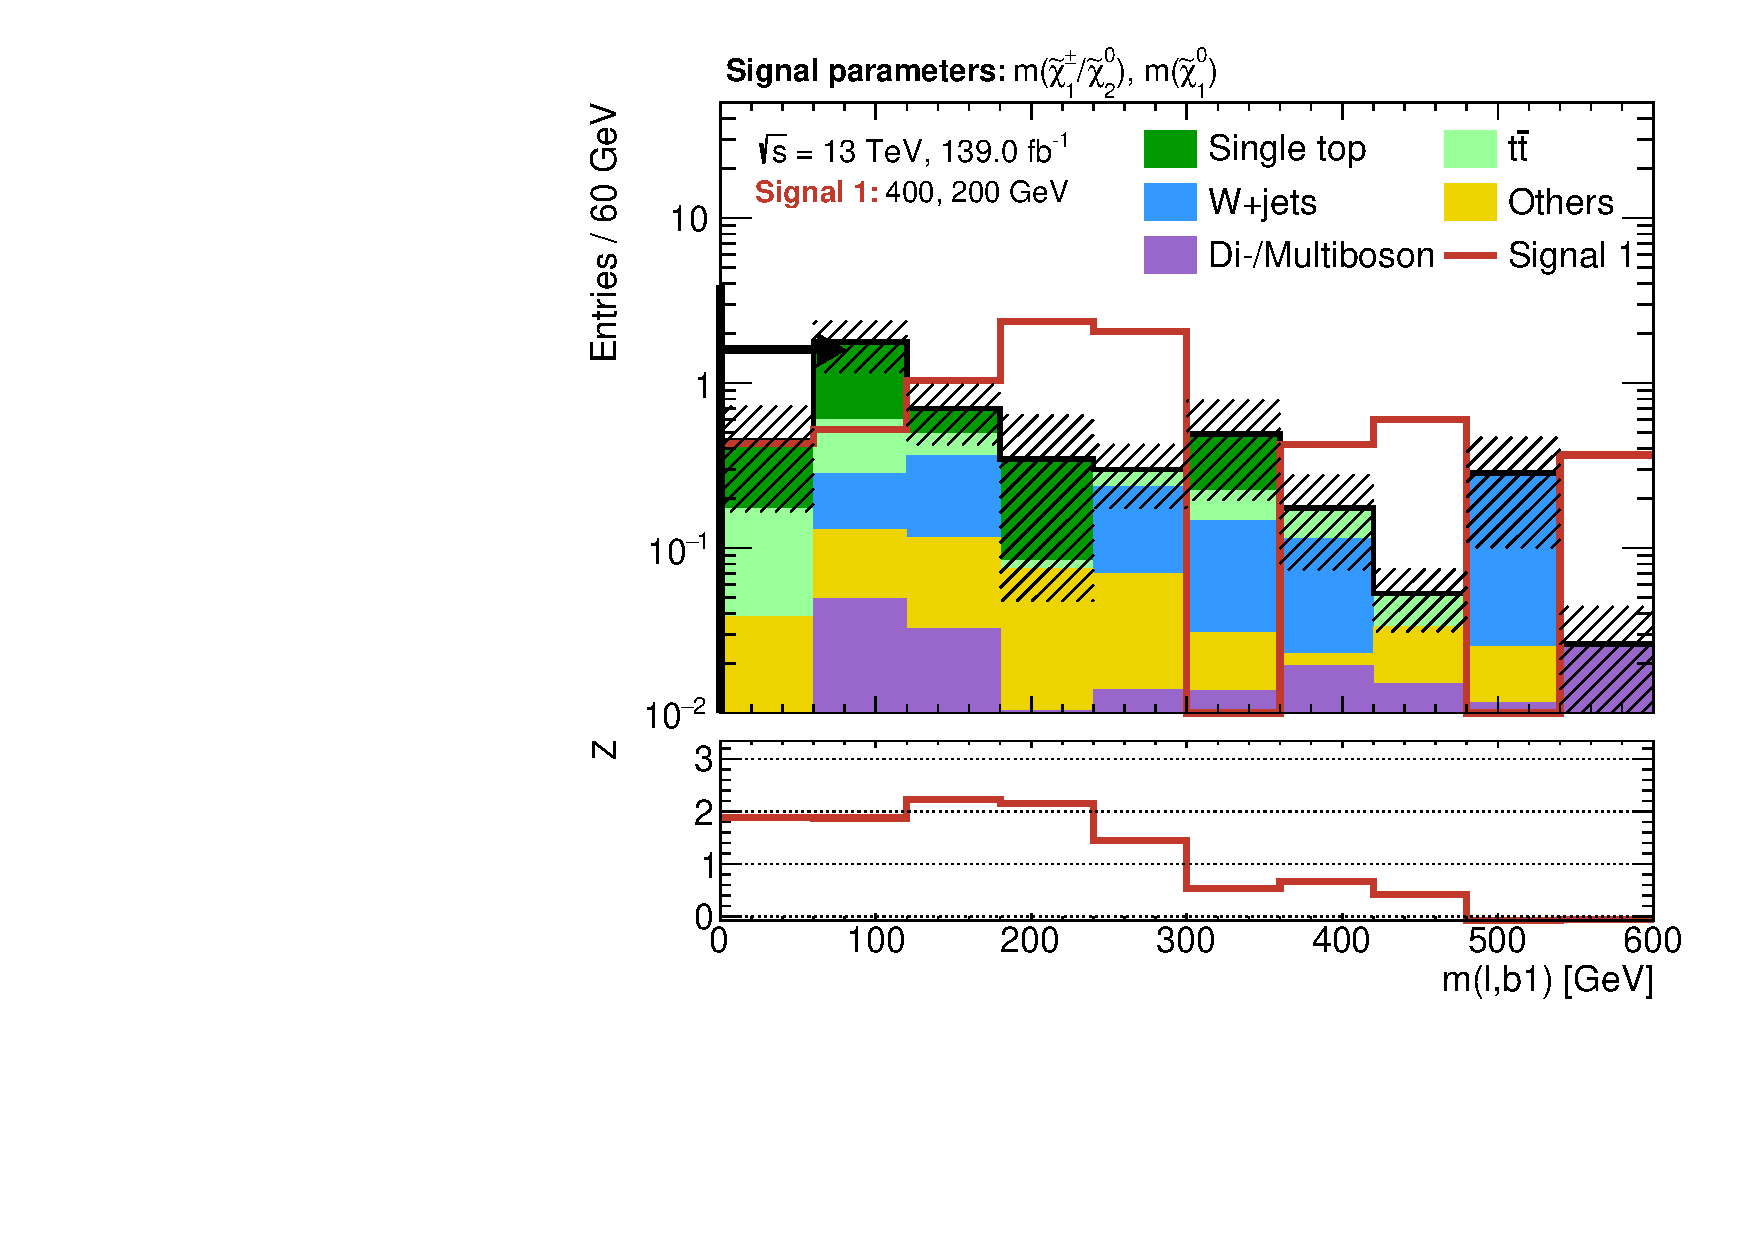
\includegraphics[width=0.9\textwidth]{N-1_cut_scan/n1_400_200/mlb1}
	\end{subfigure}\hfill
	\begin{subfigure}[b]{0.5\linewidth}
		\centering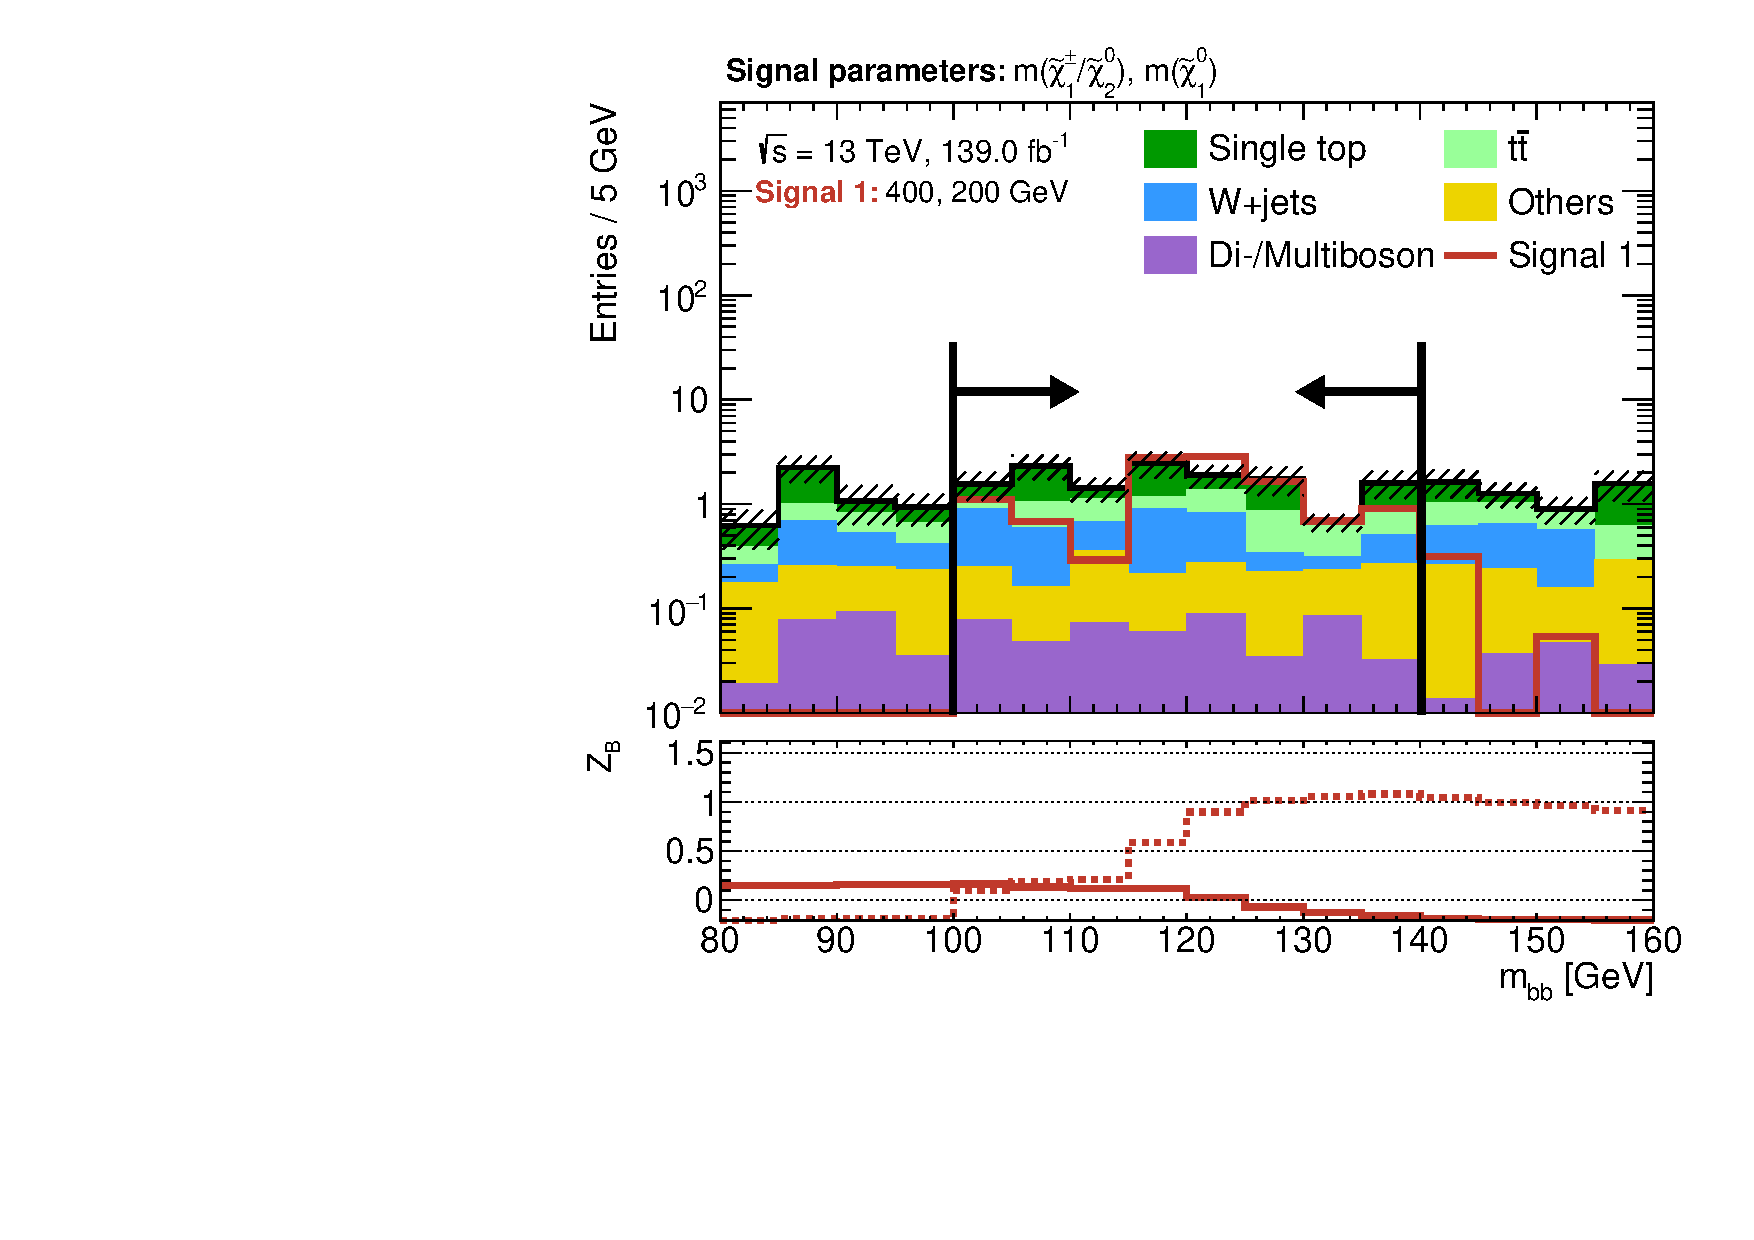
\includegraphics[width=0.9\textwidth]{N-1_cut_scan/n1_400_200/mbb_both}
	\end{subfigure}\hfill
	\begin{subfigure}[b]{0.5\linewidth}
		\centering\includegraphics[width=0.9\textwidth]{N-1_cut_scan/n1_400_200/nJet30}
	\end{subfigure}

	\caption[N-1 plots for the chosen cut combination for the (400, 200) signal point]{N-1 plots for the chosen cut combination for the $(m(\charg/\neutr), m(\lsp)) = (\SI{400}{\GeV}, \SI{200}{\GeV})$ signal point. The shaded region includes \gls{mc} statistical as well as 30\% systematic uncertainties (added in quadrature) on the background. The significance is computed using the binomial discovery significance using the uncertainty on the background.}
	\label{fig:results_n1_400_200}
\end{figure}

\begin{figure}
	\centering
	\begin{subfigure}[b]{0.5\linewidth}
		\centering\includegraphics[width=0.9\textwidth]{N-1_cut_scan/n1_300_150/mt}
	\end{subfigure}\hfill
	\begin{subfigure}[b]{0.5\linewidth}
		\centering\includegraphics[width=0.9\textwidth]{N-1_cut_scan/n1_300_150/mct}
	\end{subfigure}\hfill
	\begin{subfigure}[b]{0.5\linewidth}
		\centering\includegraphics[width=0.9\textwidth]{N-1_cut_scan/n1_300_150/met}
	\end{subfigure}\hfill
	\begin{subfigure}[b]{0.5\linewidth}
		\centering\includegraphics[width=0.9\textwidth]{N-1_cut_scan/n1_300_150/mlb1}
	\end{subfigure}\hfill
	\begin{subfigure}[b]{0.5\linewidth}
		\centering\includegraphics[width=0.9\textwidth]{N-1_cut_scan/n1_300_150/mbb_both}
	\end{subfigure}\hfill
	\begin{subfigure}[b]{0.5\linewidth}
		\centering\includegraphics[width=0.9\textwidth]{N-1_cut_scan/n1_300_150/nJet30}
	\end{subfigure}

	\caption[\textit{N}--1 plots for the chosen cut combination for the (300, 150) signal point]{\textit{N}--1 plots for the chosen cut combination for the $(m(\charg/\neutr), m(\lsp)) = (\SI{300}{\GeV}, \SI{150}{\GeV})$ signal point. The shaded region includes \gls{mc} statistical as well as 30\% systematic uncertainties (added in quadrature) on the background. The significance is computed using the binomial discovery significance using the uncertainty on the background.}
	\label{fig:results_n1_300_150}
\end{figure}

\FloatBarrier

\subsection[Impact of $\mlb$]{Impact of $\boldsymbol{\mlb}$}


As discussed in \cref{sec:variables}, the distribution of $\mlb$ has a kinematic endpoint at about $\SI{153}{\GeV}$ for $\ttbar$ and single top production events where the lepton and leading \textit{b}-jet originate from the same top quark decay. In the \gls{susy} processes considered, $\mlb$ depends on the mass-scale of the electroweakinos pair-produced, and thus offers especially good discriminative power in the high electroweakino mass regime targeted by SR-HM.

\Cref{fig:plot_mlb1_cls} illustrates the impact of adding a requirement of $\mlb > \SI{120}{\GeV}$ in SR-HM, revealing a noticeable increase in sensitivity towards high electroweakino masses. Studies have shown that the addition of $\mlb > \SI{120}{\GeV}$ to the remaining signal regions does not improve the sensitivity further.

\begin{figure}[h]
\floatbox[{\capbeside\thisfloatsetup{capbesideposition={right,center},capbesidewidth=0.35\textwidth}}]{figure}[\FBwidth]
{\caption{Comparison of different shape-fit configurations, illustrating the sensitivity increase achieved through a requirement on high $\mlb$ values in SR-HM on top of the two-dimensional shape-fit in $\mt$ and $\mct$. All exclusion limits shown are expected limits at 95\% CL, using \gls{mc} statistical and 30\% systematic uncertainties. Background estimation in the signal regions is taken directly from \gls{mc} for all \gls{sm} backgrounds.}
\label{fig:plot_mlb1_cls}}
{\includegraphics[width=0.60\textwidth]{HF/plot_mlb1}}
\end{figure}
%
%\begin{figure}
%	\centering
%	\begin{subfigure}[b]{0.5\linewidth}
%		\centering\includegraphics[width=1.0\textwidth]{HF/plot_mlb1_cls}
%		\caption{\label{fig:plot_mlb1_cls}}
%	\end{subfigure}\hfill
%
%	\caption{Comparison of different shape-fit configurations. Fig.~\subref{fig:plot_binnings_cls} compares three different two-dimensional shape-fit configurations using $3\times 3$ bins in ($\mt$, $\etmiss$), ($\mt$, $\mbb$) and ($\mt$, $\mct$). Fig.~\subref{fig:plot_mlb1_cls} illustrates the sensitivity increase achieved through a requirement on high $\mlb$ values in SR-HM on top of the two-dimensional shape-fit in $\mt$ and $\mct$. Fig.~\subref{fig:plot_2d_shapefit_cls} compares the two-dimensional shape-fit in $\mt$ and $\mct$ to the previous analysis iteration signal regions scaled to \onethirtynineifb. All exclusion limits shown are expected limits at 95\% CL, using \gls{mc} statistical and 30\% systematic uncertainty. Background estimation in the signal regions is taken directly from \gls{mc} for all \gls{sm} backgrounds.}
%	\label{fig:results_HF_scan_app}
%\end{figure}

\FloatBarrier

\graphicspath{{chapter-background/Figs/}}

\section{Background estimation}\label{app:background_estimation}

The signal contamination in all validation regions is shown in \cref{fig:signal_contaminations_VRs}. In the VR-off regions the maximum signal contamination is found to be about 7\%--13\%, depending on the requirement on $\mt$. In the VR-on regions, the maximum signal contamination amounts to about 5\%--14\%, depending again on the $\mt$-bin.


\section{Summary of results of ATLAS searches for SUSY}\label{sec:susy_summary_plot}

\Cref{fig:susy_summary_plot} provides a comprehensive summary of current results of ATLAS searches for \gls{susy}. The limits on the sparticle masses set by different searches in various models and signatures are given.

\begin{figure}
	\centering
	\begin{subfigure}[b]{0.5\linewidth}
		\centering\includegraphics[width=1.0\textwidth]{signal_contamination/plot_VR_onLM}
		\caption{VR-onLM\label{fig:signal_contamination_VRon1}}
	\end{subfigure}\hfill
	\begin{subfigure}[b]{0.5\linewidth}
		\centering\includegraphics[width=1.0\textwidth]{signal_contamination/plot_VR_offLM}
		\caption{VR-offLM\label{fig:signal_contamination_VRoff1}}
	\end{subfigure}\hfill
	\par\medskip
	\begin{subfigure}[b]{0.5\linewidth}
		\centering\includegraphics[width=1.0\textwidth]{signal_contamination/plot_VR_onMM}
		\caption{VR-onMM\label{fig:signal_contamination_VRon2}}
	\end{subfigure}\hfill
	\begin{subfigure}[b]{0.5\linewidth}
		\centering\includegraphics[width=1.0\textwidth]{signal_contamination/plot_VR_offMM}
		\caption{VR-offMM\label{fig:signal_contamination_VRoff2}}
	\end{subfigure}\hfill
	\begin{subfigure}[b]{0.5\linewidth}
		\centering\includegraphics[width=1.0\textwidth]{signal_contamination/plot_VR_onHM}
		\caption{VR-onHM\label{fig:signal_contaminations_VRon3}}
	\end{subfigure}\hfill
	\begin{subfigure}[b]{0.5\linewidth}
		\centering\includegraphics[width=1.0\textwidth]{signal_contamination/plot_VR_offHM}
		\caption{VR-offHM\label{fig:signal_contaminations_VRoff3}}
	\end{subfigure}\hfill

	\caption{Signal contamination (shown on the \textit{z-axis}) for all \glspl{vr} throughout the signal grid. The space between the signal points (indicated by the black circles) is interpolated using Delaunay triangles.}
	\label{fig:signal_contaminations_VRs}
\end{figure}



\graphicspath{{chapter-results/Figs/Vector/}{chapter-results/Figs/}}


\begin{sidewaysfigure}[ht]
	\centering\includegraphics[width=0.9\textwidth]{susy_summary}
	\caption{Summary of the results of ATLAS searches for \gls{susy}. A representative selection of the available search results is shown. Results are given with respect to the nominal cross section. In some cases additional dependencies are indicated by darker bands showing different model parameters. Figure adapted from \reference\cite{ATL-PHYS-PUB-2021-007}.}
	\label{fig:susy_summary_plot}
\end{sidewaysfigure}



